\documentclass{article}
% --------------------------------------------
% Theorem Environments and Math Setup
% --------------------------------------------
\usepackage{amsthm}
\usepackage{amsmath, amssymb}
\usepackage{mathtools}
\usepackage{bm}              % for bold math symbols
\usepackage{bbm}             % for indicator functions and blackboard 1
\usepackage{mathrsfs}        % for nice script letters
\usepackage{upgreek}         % for upright greek letters like \upvarphi
\usepackage{dsfont}          % for \mathds{1}
\usepackage{graphicx}        % for \includegraphics
\usepackage{subcaption}      % for subfigures

% Theorem environments
\theoremstyle{definition}
\newtheorem{definition}{Definition}[section]

\theoremstyle{plain}
\newtheorem{theorem}[definition]{Theorem}
\newtheorem{lemma}[definition]{Lemma}
\newtheorem{proposition}[definition]{Proposition}
\newtheorem{corollary}[definition]{Corollary}

\theoremstyle{remark}
\newtheorem{remark}[definition]{Remark}
\newtheorem{example}[definition]{Example}

% Proof environment already included via amsthm
% For "QED" symbol at end of proofs
\renewcommand{\qedsymbol}{$\blacksquare$}

% Shortcuts
\newcommand{\R}{\mathbb{R}}
\newcommand{\C}{\mathbb{C}}
\newcommand{\N}{\mathbb{N}}
\newcommand{\Z}{\mathbb{Z}}
\newcommand{\eps}{\varepsilon}
\newcommand{\norm}[1]{\left\lVert #1 \right\rVert}
\newcommand{\abs}[1]{\left\lvert #1 \right\rvert}
\newcommand{\scalar}[2]{\left\langle #1, #2 \right\rangle}

% Domains and function spaces
\newcommand{\Ltwo}{L^2(\Omega)}
\newcommand{\Hone}{H^1(\Omega)}
\newcommand{\Honezero}{H_0^1(\Omega)}

% make command that \dt is \dt in math mode
\newcommand{\dt}{\text{dt}}

\setlength{\parindent}{0pt}

\begin{document}

\title{Waves, Wires, and Weights: Numerical Adventures with the Schrödinger Equation}
\author{Simon Wenchel and Lasse Kreimendahl}
\date{\today}
\maketitle

\tableofcontents

\newpage

\section{Introduction}

The time-dependent Schrödinger equation lies at the heart of quantum mechanics, dictating how the state of a quantum system evolves under the influence of potential energy landscapes. In contrast to classical mechanics, which predicts trajectories, the Schrödinger equation predicts wave functions, whose squared modulus yields probability densities. This shift from deterministic paths to probabilistic amplitudes marks a fundamental departure from classical intuition.

\begin{figure}[h]
    \centering
    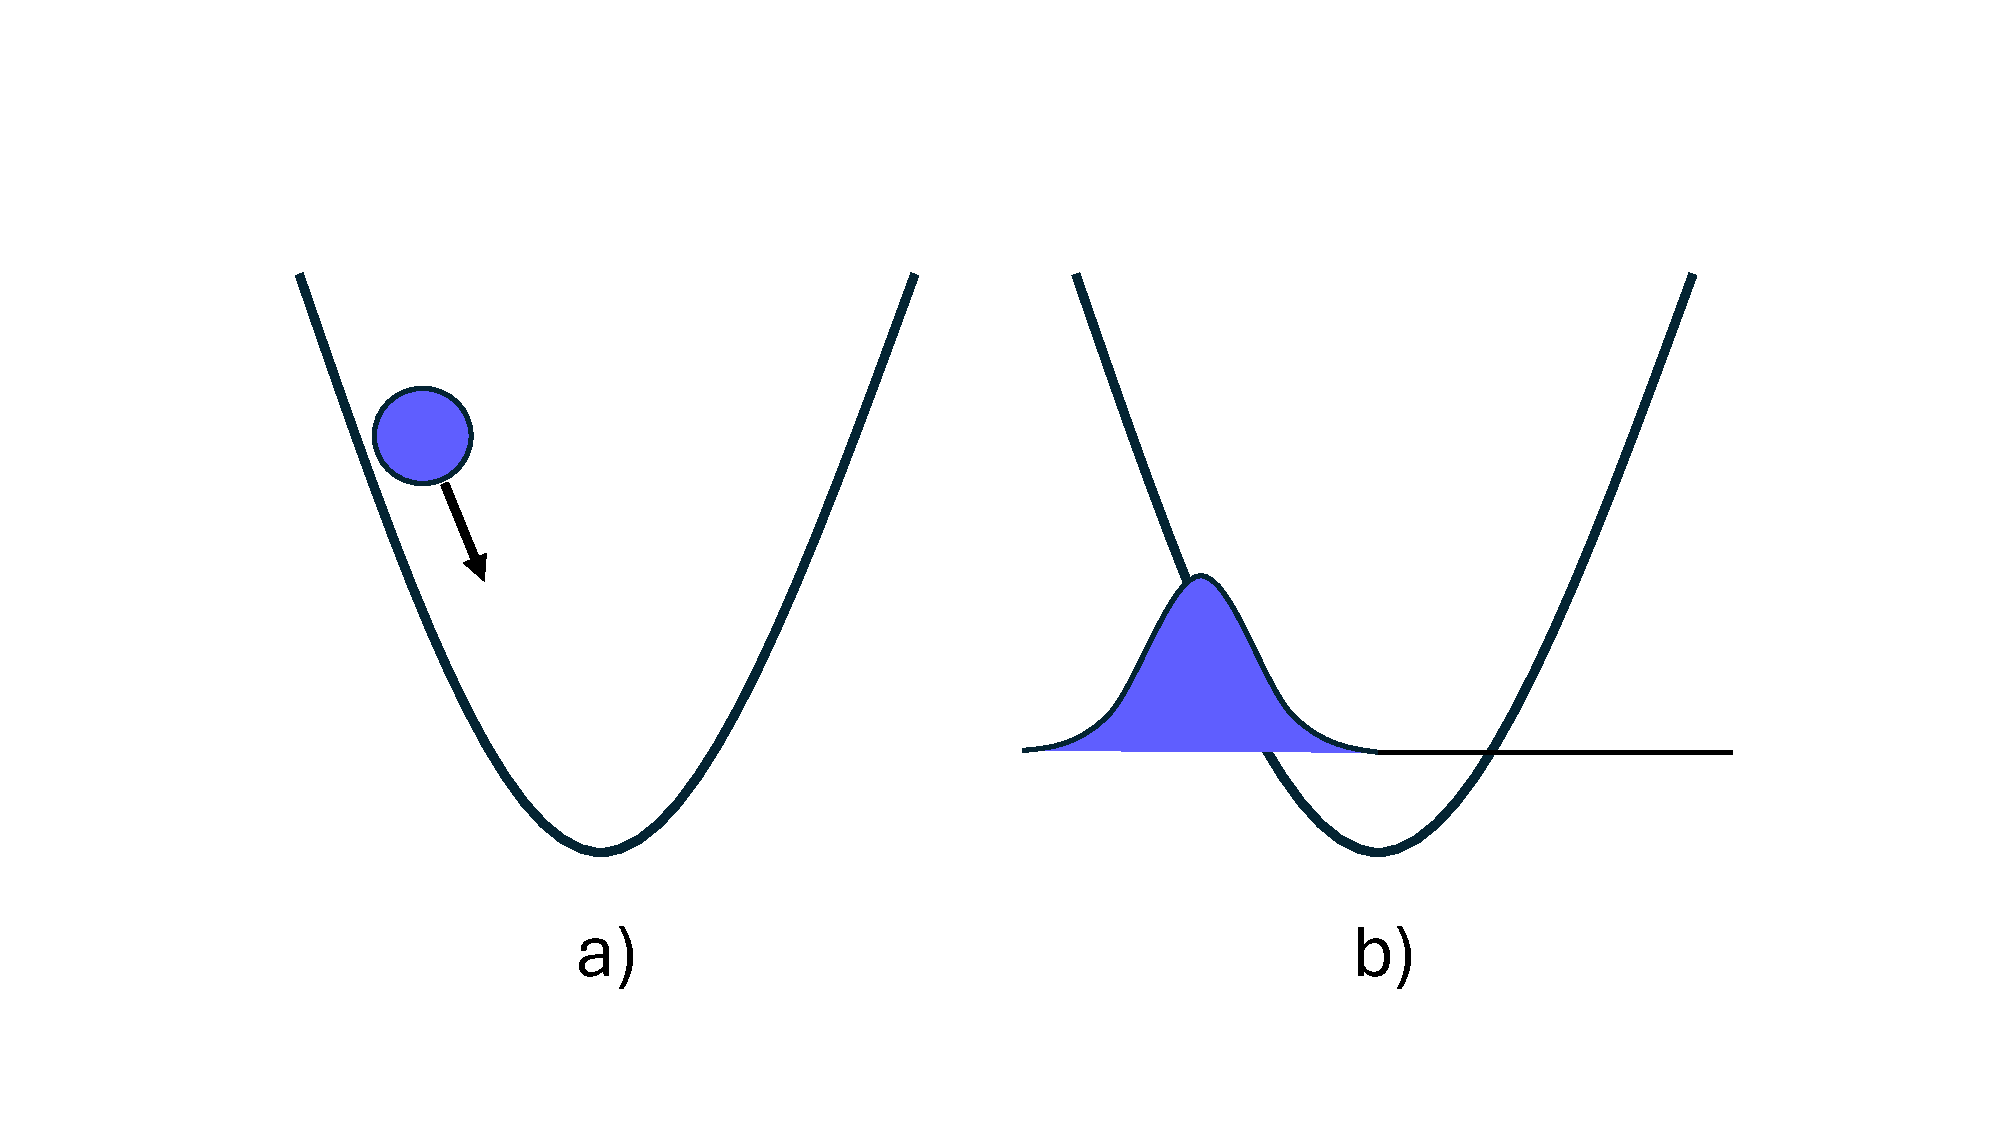
\includegraphics[width=0.8\textwidth]{figures/Figure1.pdf}
    \caption{}
    \label{fig:fig1}
\end{figure}

From fundamental atomic models to emergent quantum technologies, the ability to solve the Schrödinger equation accurately and efficiently is essential for predicting quantum behavior. Yet, in most realistic settings, analytic solutions are unavailable. This necessitates the development of robust numerical approaches.

In molecular systems, the Schrödinger equation governs the motion of nuclei on potential energy surfaces obtained from electronic structure calculations. Within the Born-Oppenheimer approximation, these nuclei behave as quantum particles subject to high-dimensional, often anharmonic potentials. For example, when modeling the movement of atoms within a molecule, it is common to reduce the full-dimensional problem to a few key internal coordinates, such as bond stretching or rotations. Even in such simplified spaces, the time evolution of a quantum state can reveal complex phenomena such as tunneling (where a particle passes through a potential barrier it classically could not cross), interference (where overlapping wave functions amplify or cancel each other), or wave packet spreading (the dispersion of a localized quantum state over time)—none of which are accessible through classical approximations.

\begin{figure}[h]
    \centering
    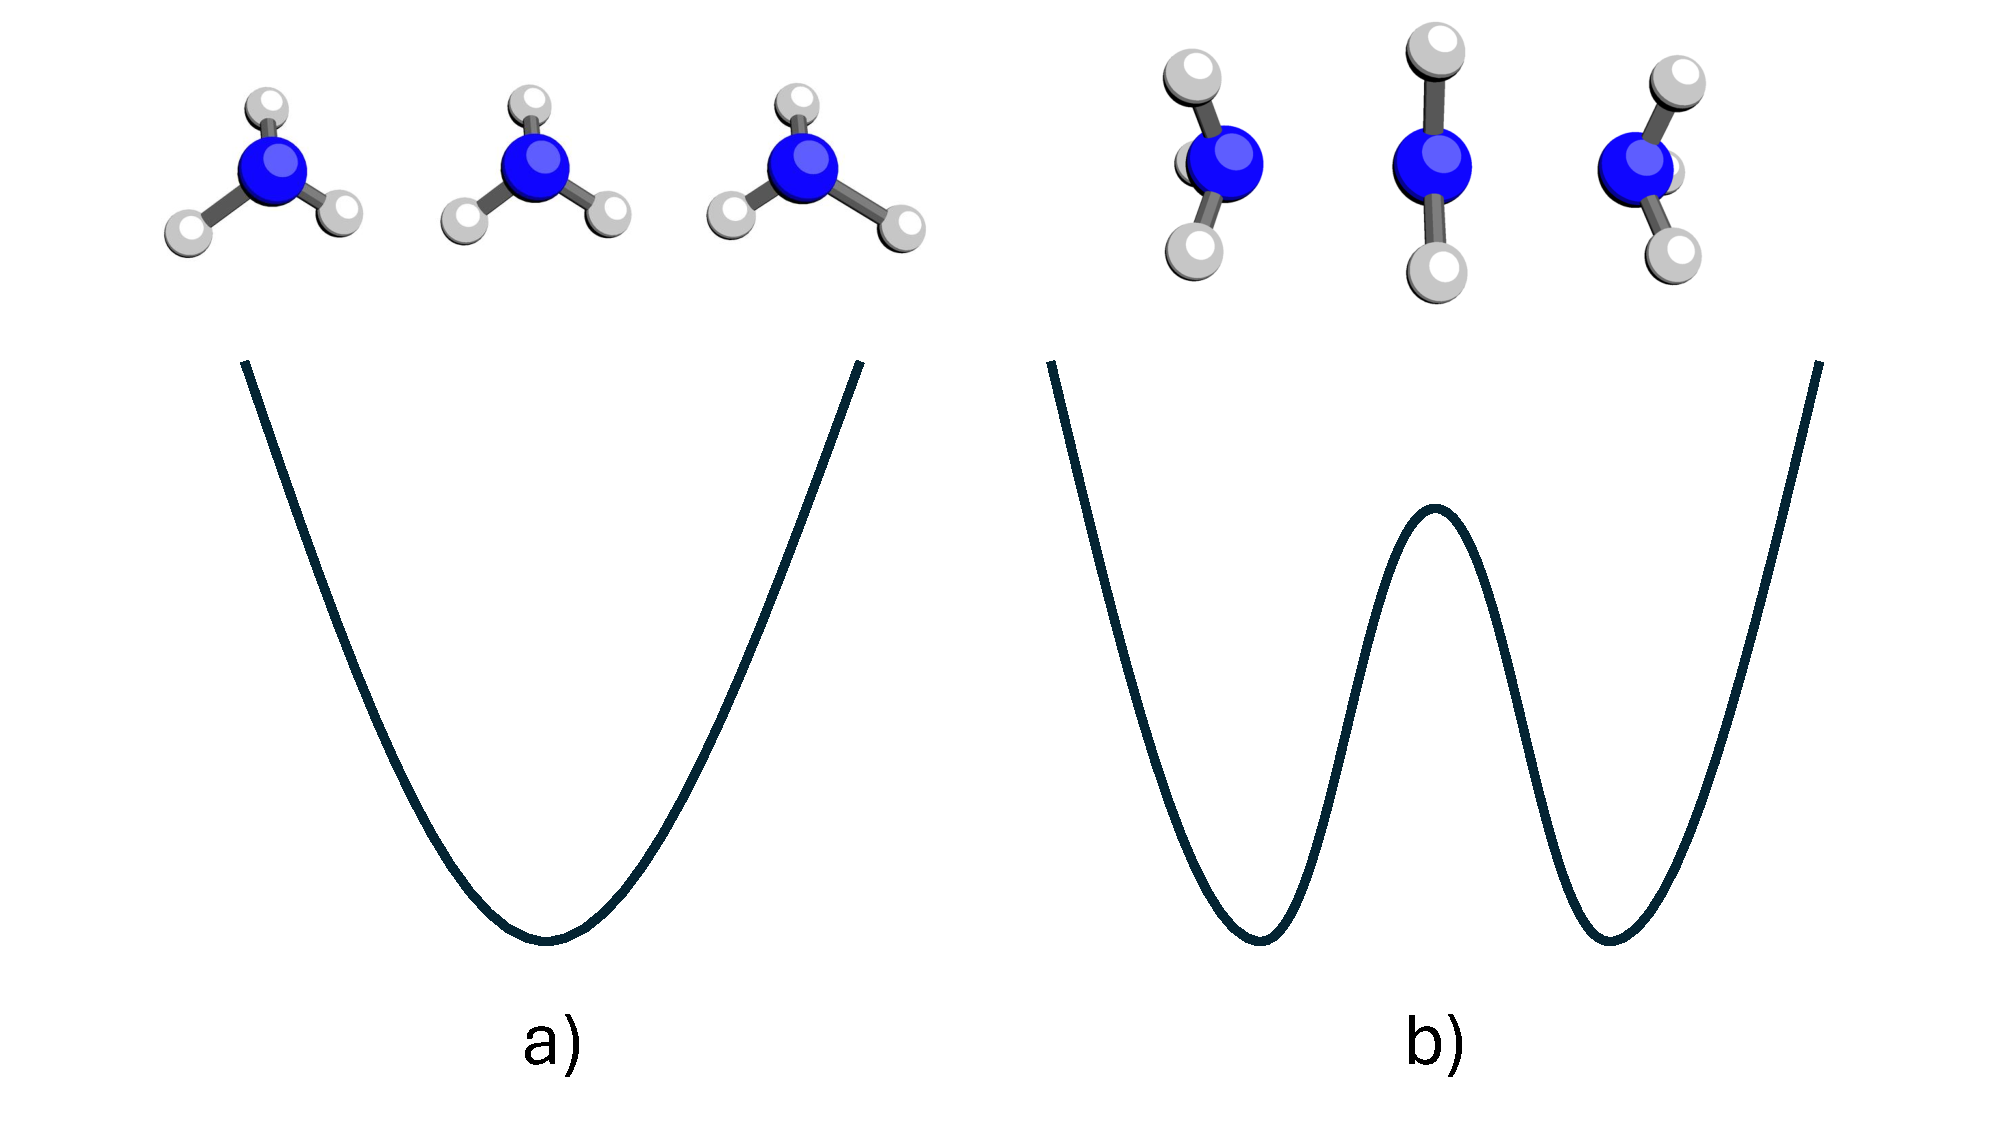
\includegraphics[width=0.8\textwidth]{figures/Figure2.pdf}
    \caption{}
    \label{fig:fig2}
\end{figure}

This report investigates the numerical solution of the time-dependent Schrödinger equation in two spatial dimensions, a setting that permits the exploration of realistic molecular scenarios while maintaining computational tractability. Specifically, we consider model systems where the potential energy surface encodes features representative of atomic motions, reactive pathways, or coupled physical effects.

To address this problem, we compare two distinct numerical strategies. The first is the finite element method (FEM), a classical and rigorously grounded approach based on variational formulations. The second leverages recent advances in machine learning: physics-informed neural networks (PINNs), which approximate the solution by minimizing the residual of the governing equations within a data-driven framework. While FEM offers precision and theoretical guarantees, PINNs provide flexibility and mesh-free generalization—particularly attractive for high-dimensional or inverse problems.

Through this dual lens, the report aims to highlight both the challenges and opportunities inherent in solving quantum dynamical equations numerically, and to evaluate the strengths of different computational paradigms in a physically meaningful context.

\section{Finite Element Method}

\subsection*{Model Problem: Schrödinger Equation}

The Schrödinger equation is a second-order partial differential equation that describes the time evolution of a quantum system, represented by its wave function. \\
Let $\Omega \subset \mathbb{R}^n$ be a bounded Lipschitz domain and let $V : \Omega \times [0,T] \to \mathbb{R}$ be a given potential. We say that a function
\[
u : \Omega \times [0,T] \to \mathbb{C}
\]
is a \textbf{solution to the time-dependent Schrödinger equation, with homogeneous Dirichlet boundary conditions} if it satisfies the following system of equations:
\begin{align*}
    i \partial_t u(x,t) &= - \Delta u(x,t) + V(x,t) u(x,t), \quad x \in \Omega, \ t > 0,\\
    \partial_t u(x,0) &= u_0(x), \quad x \in \Omega,\\
    \quad u(x,t) &= 0, \quad x \in \partial \Omega, \ t > 0,
\end{align*}


where $\Delta$ is the Laplacian operator, $V(x,t)$ is a potential, $\partial \Omega$ is the boundary of the domain $\Omega$, and $u_0(x)$ is the initial condition at time $t=0$. 


Should we include this description?\\
The function $u(x,t)$ represents the wave function of the quantum system at position $x$ and time $t$. The term $i \partial_t u(x,t)$ represents the time evolution of the wave function, while the term $-\Delta u(x,t)$ accounts for the kinetic energy of the system. The potential term $V(x,t) u(x,t)$ describes the interaction of the wave function with an external potential.


\subsection*{Weak Formulation of Schrödinger's Equation}
To derive the weak formulation of the time dependent Schrödinger equation, we multiply the equation by $\bar{v}$ the complex conjugate of the test function $v(x,t) \in H_0^1(\Omega; \mathbb{C})$ and integrate over the domain $\Omega$. 
\paragraph{Sobolev Space with Complex Values}
Let $\Omega \subset \mathbb{R}^d$ be a bounded Lipschitz domain. We define the complex Sobolev space
\[
H_0^1(\Omega; \mathbb{C}) := \left\{ u \in L^2(\Omega; \mathbb{C}) \ \middle| \ \nabla u \in L^2(\Omega; \mathbb{C}^d), \ u|_{\partial \Omega} = 0 \right\}.
\]
This space is equipped with the inner product
\[
\langle u, v \rangle_{H_0^1()} := \int_\Omega \nabla u \cdot \nabla \overline{v} \, dx + \int_\Omega u \, \overline{v} \, dx,
\]
and the associated norm
\[
\|u\|_{H_0^1} := \sqrt{ \langle u, u \rangle_{H_0^1} }.
\]
% The Sobolev space $H_0^1(\Omega; \mathbb{C})$ consists of functions that are square integrable and have square integrable weak derivatives, with the additional condition that they vanish on the boundary $\partial \Omega$.\\
By utilizing Greens' identity, we can transform the second order differential equation into a first order weak formulation:
\begin{align*}
  \int_{\Omega} \Delta u \bar{v} \, dx &= \int_{\Omega} \nabla u \cdot \nabla \bar{v} \, dx - \int_{\partial \Omega} \nabla u \cdot n \bar{v} \, ds,\\
  &= \int_{\Omega} \nabla u \cdot \nabla \bar{v} \, dx, \quad (\text{since } u \text{ vanishes on } \partial \Omega).
\end{align*}
This leads to the weak formulation of the Schrödinger equation:
\begin{align*}
    i \int_{\Omega} \left( \partial_t u \right) \bar{v} \, dx = - \int_{\Omega} \nabla u \cdot \nabla \bar{v} \, dx + \int_{\Omega} V(x,t) u \bar{v} \, dx.
\end{align*}
We take the complex conjugate of the test function $v$ to ensure that the formulation aligns with the sesquilinear inner product in Hilbert spaces like $L^2(\Omega; \mathbb{C})$ and $H_0^1(\Omega; \mathbb{C})$.


\subsection*{Time Integration with the Euler Method}
The Euler method is a simple and widely used numerical method for solving  differential equations.
It approximates the time derivative with a first order finite difference scheme. In the following we will use the backward Euler method, which gives an approximation of the time derivative as follows:
\begin{align*}
    \partial_t u(x,t) \approx \frac{u^{t + \dt} - u^t}{\dt},
\end{align*}
The backward euler method allows us to solve the Schrödinger equation iteratively in each time step by finite elements method in space.
The time resolution is controlled by the time step size $\dt$, where $t$ is the current time and $t + \dt$ is the next time step.

The backward Euler method has a remaining error of order $\mathcal{O}(\dt)$, which means that the error decreases linearly with the time step size. 
This is sufficient for many applications, but for higher accuracy, higher order methods such as the Crank-Nicolson method or Runge-Kutta methods can be used.


\subsection*{Weak Formulation with Backward Euler Method}
The time-discrete weak form of the Schrödinger equation becomes:
\begin{align*}
    i \int_{\Omega} \left( \frac{u^{t + \dt} - u^t}{\dt} \right) \bar{v} \, dx = - \int_{\Omega} \nabla u^{t + \dt} \cdot \nabla \bar{v} \, dx + \int_{\Omega} V(x,t) u^{t+\dt} \bar{v} \, dx
\end{align*}
By rearranging, the  weak formulation takes the form, with implicit terms on the left and explicit (known) terms on the right:
\begin{align*}
    i \int_{\Omega} u^{t + \dt} \bar{v} - \dt \int_{\Omega}  u^{t+\dt} \bar{v} V(x,t)  \, dx + \dt \int_{\Omega} \nabla u^{t + \dt} \cdot \nabla \bar{v} &= i \int_{\Omega} u^t \bar{v} \, dx ,\\
    a(u^{t + \dt}, v) &= L(v),
\end{align*}
which can be solved iteratively for $u^{t + \dt}$ in each time step.


% make note in red that i describe u and v dependent of x,t and t+dt is next timestep
% Note: In the following, we will denote the dependence of $u$ and $v$ on $x$ and $t$ explicitly, while $t + \dt$ refers to the next time step.



\subsection*{Existence and Uniqueness via the Lax-Milgram Theorem in Complex Hilbert Spaces}
To establish the existence and uniqueness of solutions to the weak formulation of the Schrödinger equation, we can apply the Lax-Milgram theorem. 
This theorem provides conditions under which a sesquilinear form defines a unique solution to a linear functional equation in a Hilbert space.
\begin{theorem}
[Lax-Milgram Theorem]
Let $H$ be a complex Hilbert space with inner product $\langle \cdot, \cdot \rangle$ and norm $\| \cdot \|_H$. Let $a : H \times H \to \mathbb{C}$ be a sesquilinear form, i.e.,
\[
a(\cdot, v) \text{ is linear for all } v \in H, \quad a(u, \cdot) \text{ is conjugate-linear for all } u \in H.
\]
Suppose that:
\begin{enumerate}
    \item \textbf{Boundedness of the sesquilinear form:} There exists $M > 0$ such that
    \[
    |a(u, v)| \leq M \|u\|_H \|v\|_H \quad \text{for all } u, v \in H.
    \]
    \item \textbf{Boundedness of the linear form:} There exists $C > 0$ such that
    \[
    |L(v)| \leq C \|v\|_H \quad \text{for all } v \in H.
    \]
    \item \textbf{Coercivity:} There exists $\alpha > 0$ such that
    \[
    \Re \, a(u, u) \geq \alpha \|u\|_H^2 \quad \text{for all } u \in H.
    \]
\end{enumerate}
Then for every bounded linear functional $L \in H^*$, there exists a unique $u \in H$ such that
\[
a(u, v) = L(v) \quad \text{for all } v \in H.
\]
\end{theorem}


\subsection*{Application of the Lax-Milgram Theorem to the Discrete Schrödinger Equation}
In the following, we will show the conditions of the Lax-Milgram theorem are satisfied for the sesquilinear form $a(u, v)$ and the linear functional $L(v)$, such that the existence and uniqueness of the solution to the weak formulation of the Schrödinger equation is guaranteed.\\
As we have already established, the Sobolev space $H_0^1(\Omega; \mathbb{C})$ is a Hilbert space with the inner product:
\[
\langle u, v \rangle_{H_0^1(\Omega)} := \int_\Omega \nabla u \cdot \nabla \overline{v} \, dx + \int_\Omega u \, \overline{v} \, dx.
\]
% \subsection*{Scalar Product in $H_0^1(\Omega; \mathbb{C})$}

% We define the scalar product
% \[
% \langle u, v \rangle_{H_0^1} := \int_\Omega \nabla u \cdot \nabla \overline{v} \, dx + \int_\Omega u \, \overline{v} \, dx.
% \]
% This is a valid sesquilinear inner product because:
% \begin{itemize}
%   \item It is \textbf{linear} in the first argument: $\langle \lambda u_1 + \mu u_2, v \rangle = \lambda \langle u_1, v \rangle + \mu \langle u_2, v \rangle$ for all $\lambda, \mu \in \mathbb{C}$.
%   \item It is \textbf{conjugate-linear} in the second argument.
%   \item It is \textbf{Hermitian}: $\langle u, v \rangle = \overline{\langle v, u \rangle}$.
%   \item It is \textbf{positive-definite}: $\langle u, u \rangle = 0$ implies $u = 0$ in $H_0^1$.
% \end{itemize}
% Hence, $(H_0^1(\Omega; \mathbb{C}), \langle \cdot, \cdot \rangle_{H_0^1})$ is a Hilbert space.

\subsubsection*{Boundedness of the Sesquilinear and Linear Form.}

\begin{lemma}[Boundedness of $a(u, v)$]
Let $u, v \in H_0^1(\Omega; \mathbb{C})$, $V \in L^\infty(\Omega)$ and $\tau > 0$. Then the sesquilinear form $a(u, v)$ is bounded, i.e., there exists $M > 0$ such that
\[
|a(u, v)| \leq M \|u\|_{H_0^1} \|v\|_{H_0^1}.
\]
\end{lemma}

\begin{proof}
By triangle inequality, we can split the sesquilinear form into three terms:
\[
|a(u, v)| \leq \left|\int_\Omega \nabla u \cdot \nabla \overline{v} \, dx \right| + \left| \frac{i}{\dt} \int_\Omega u \, \overline{v} \, dx \right| + \left| \int_\Omega V(x,t) u^{t + \dt} \bar{v} \, dx \right|.
\]
We estimate each term separately.

\textbf{(1) Stiffness term:}
\begin{align*}
  \left| \int_\Omega \nabla u \cdot \nabla \overline{v} \, dx \right| &\leq \int_\Omega |\nabla u| |\nabla \overline{v}| \, dx = \int_\Omega |\nabla u| |\nabla \overline{v}| \, dx = \int_\Omega |\nabla u| |\nabla v| \, dx \\
  & \leq \|\nabla u\|_{L^2(\Omega)} \|\nabla v\|_{L^2(\Omega)}
\quad \text{(by Cauchy-Schwarz in } L^2(\Omega; \mathbb{C}^d) \text{)}.
\end{align*}


\textbf{(2) Mass term:}
\begin{align*}
\left| \int_\Omega \frac{i}{\dt} u \, \overline{v} \, dx \right|
&= \frac{1}{\dt} \left| \int_\Omega u \, \overline{v} \, dx \right| \leq \frac{1}{\dt} \int_\Omega |u| |v| \, dx \\
& \leq \frac{1}{\dt} \|u\|_{L^2(\Omega)} \|v\|_{L^2(\Omega)} \quad \text{(again by Cauchy-Schwarz)}.
\end{align*}


\textbf{(3) Potential term:}
\begin{align*}
\left| \int_\Omega V(x,t) u^{t + \dt} \bar{v} \, dx \right| &\leq \|V\|_{L^\infty(\Omega )} \int_\Omega |u^{t + \dt}| |\bar{v}| \, dx \\
&\leq \|V\|_{L^\infty(\Omega)} \|u^{t + \dt}\|_{L^2(\Omega)} \|v\|_{L^2(\Omega)}.
\end{align*}

\textbf{Combining all terms:}
\begin{align*}
|a(u, v)| &\leq \|\nabla u\|_{L^2} \|\nabla v\|_{L^2} + \frac{1}{\dt} \|u\|_{L^2} \|v\|_{L^2} + \|V\|_{L^\infty} \|u^{t + \dt}\|_{L^2} \|v\|_{L^2}\\
& \leq M \left( \|\nabla u\|_{L^2} \|\nabla v\|_{L^2} + \|u\|_{L^2} \|v\|_{L^2} \right),\\
&\leq M \|u\|_{H_0^1} \|v\|_{H_0^1}, \quad \text{(by Cauchy-Schwarz)}
\end{align*}
where \( M = \max\left(1, \frac{1}{\dt} + \|V\|_{L^\infty}\right) \).
% The last step is valid because:
% \begin{align*}
%   ab+cd &\leq \sqrt{a^2 + c^2} \sqrt{b^2 + d^2} = \|(a,c)\| \|(b,d)\| \quad \text{(by Cauchy-Schwarz)},
% \end{align*}
% where $a = \|\nabla u\|_{L^2}$, $b = \|u\|_{L^2}$, $c = \|\nabla v\|_{L^2}$, and $d = \|v\|_{L^2}$.
% \[
% |a(u, v)| \leq \|\nabla u\|_{L^2} \|\nabla v\|_{L^2}
% + \frac{1}{\dt} \|u\|_{L^2} \|v\|_{L^2}.
% \]

\end{proof}
% \[
% |a(u, v)| \leq \|\nabla u\|_{L^2} \|\nabla v\|_{L^2}
% + \frac{1}{\dt} \|u\|_{L^2} \|v\|_{L^2}.
% \]

% Recalling the definition of the \(H_0^1\) norm:
% \[
% \|u\|_{H_0^1}^2 := \|\nabla u\|_{L^2}^2 + \|u\|_{L^2}^2.
% \]
% \[
% a(u, v) = \int_\Omega \nabla u \cdot \nabla \overline{v} \, dx + \int_\Omega  \frac{i}{\tau}  u \, \overline{v} \, dx
% \]
% is coercive on $H_0^1(\Omega; \mathbb{C})$, i.e., there exists $\alpha > 0$ such that
% \[
% \Re a(u, u) \geq \alpha \|u\|_{H_0^1}^2 \quad \forall u \in H_0^1(\Omega; \mathbb{C}).
% \]

% \begin{proof}
% We compute the real part of $a(u,u)$:
% \begin{align*}
% \Re a(u, u)
% &= \Re \left( \int_\Omega |\nabla u|^2 \, dx + \int_\Omega  \frac{i}{\dt} |u|^2 \, dx \right) = \int_\Omega |\nabla u|^2 \, dx \\
% &= ||\nabla u||_{L^2(\Omega)}^2 \\
% % &\geq C \int_\Omega |u|^2 \, dx \quad \text{(by Poincaré inequality)}.\\
% % &= ||u||_{L^2(\Omega)}^2.
% \end{align*}

% By recalling the definition of the \(H_0^1\) norm:
% \[
% ||u||_{H_0^1(\Omega)}^2 = ||\nabla u||_{L^2(\Omega)}^2 + ||u||_{L^2(\Omega)}^2,
% \]
% we can transform achieve the coercivity condition by using the Poincaré inequality.
% \begin{align*}
%   ||\nabla u||_{L^2(\Omega)}^2 &= \frac{1}{2} || \nabla u||_{L^2(\Omega)}^2 + \frac{1}{2} || \nabla u||_{L^2(\Omega)}^2\\
%   & \geq \frac{1}{2} ||u||_{L^2(\Omega)}^2 + \frac{1}{2} ||\nabla u||_{L^2(\Omega)}^2 \text{(by Poincaré inequality)} \\
%   & = \frac{1}{2} ||u||_{H_0^1(\Omega)}^2.
% \end{align*}
% \end{proof}

% \begin{lemma}[Boundedness of the linear form]
% Let $\psi^{n-1} \in L^2(\Omega; \mathbb{C})$ be given. Then the linear functional
% \[
% L(v) := \int_\Omega \frac{i}{\tau} \psi^{n-1}(x) \, \overline{v(x)} \, dx
% \]
% is bounded on $H_0^1(\Omega; \mathbb{C})$. That is, there exists a constant $C > 0$ such that
% \[
% |L(v)| \leq C \|v\|_{H_0^1(\Omega)} \quad \forall v \in H_0^1(\Omega; \mathbb{C}).
% \]
% \end{lemma}

\begin{lemma}[Boundedness of the linear form]
Let $u^t \in L^2(\Omega; \mathbb{C})$ be given. Then the linear functional
\[
L(v) := \frac{i}{\dt}\int_\Omega  u^{t} \, \overline{v} \, dx
\]
is bounded on $H_0^1(\Omega; \mathbb{C})$. That is, there exists a constant $C > 0$ such that
\[
|L(v)| \leq C \|v\|_{H_0^1(\Omega)} \quad \forall v \in H_0^1(\Omega; \mathbb{C}).
\]
\end{lemma}

% \begin{lemma}[Boundedness of the linear form]
% Let $u^{t} \in L^2(\Omega; \mathbb{C})$ and $V \in L^\infty(\Omega \times [0,T]; \mathbb{R})$. Define the linear form
% \[
% L(v) := i \int_\Omega u^{t}(x) \, \overline{v(x)} \, dx + \Delta t \int_\Omega V(x,t) \, u^{t}(x) \, \overline{v(x)} \, dx.
% \]
% Then there exists a constant $C > 0$ (depending on $\|u^{t}\|_{L^2}$ and $\|V\|_{L^\infty}$) such that
% \[
% |L(v)| \leq C \|v\|_{H_0^1(\Omega)} \quad \forall v \in H_0^1(\Omega; \mathbb{C}).
% \]
% \end{lemma}

\begin{proof}
We estimate each term separately using the Cauchy-Schwarz and Hölder inequalities.
\begin{align*}
|L(v)| &\leq \left| \frac{i}{\dt} \int_\Omega u^{t}(x) \, \overline{v(x)} \, dx\right|= \frac{1}{\dt}\left| \int_\Omega u^{t}(x) \, \overline{v(x)} \, dx \right|\\
&\leq \frac{1}{\dt}\int_\Omega |u^{t}(x)| \, |v(x)| \, dx  \quad \text{(by triangle inequality)} \\
&\leq \frac{1}{\dt}\|u^{t}\|_{L^2(\Omega)} \|v\|_{L^2(\Omega)} \quad \text{(by Cauchy-Schwarz inequality)}.
\end{align*}


% Combining both:
% \[
% |L(v)| \leq \left(1 + \dt \|V\|_{L^\infty(\Omega)}\right) \|u^{t-1}\|_{L^2(\Omega)} \|v\|_{L^2(\Omega)}.
% \]
As in the last proof we can split $\|v\|_{L^2(\Omega)} = \frac{1}{2} \|v\|_{L^2(\Omega)}^2 + \frac{1}{2} \|v\|_{L^2(\Omega)}^2$ and use the Poincaré inequality which gives us:
\[
|L(v)| \leq \frac{\tilde{C}}{2} \left(\|\nabla v\|_{L^2(\Omega)}^2 + \|v\|_{L^2(\Omega)}^2 \right) \leq C \|v\|_{H_0^1(\Omega)}^2,
\]
where \( C = \frac{1}{2\dt}\|u^{t}\|_{L^2(\Omega)} \).

Hence, \( L \) is bounded.
\end{proof}

\subsubsection*{Coercivity of the Sesquilinear Form}

\begin{lemma}
[Coercivity of the sesquilinear form]
Let \( a(u, v) \) be the sesquilinear form defined by
\[
a(u, v) = \int_\Omega \nabla u \cdot \nabla \overline{v} \, dx + \frac{i}{\dt} \int_\Omega  u \, \overline{v} \, dx - \int_\Omega V(x,t) u \, \overline{v} \, dx.
\]
Then there exists a constant \( \alpha > 0 \) such that
\[
\Re a(u, u) \geq \alpha \|u\|_{H_0^1(\Omega)}^2 \quad \forall u \in H_0^1(\Omega; \mathbb{C}).
\]
\end{lemma}
\begin{proof}
We compute the real part of $a(u,u)$:
Note: check again for minus signs looks weird
\begin{align*}
\Re a(u, u)
&= \Re \left( \int_\Omega |\nabla u|^2 \, dx + \frac{i}{\dt}\int_\Omega   |u|^2 \, dx - \int_\Omega V(x,t) u \, \overline{u} \, dx \right) \\
&=  \int_\Omega |\nabla u|^2 \, dx - \int_\Omega V(x,t) |u|^2 \, dx \\
&= ||\nabla u||_{L^2(\Omega)}^2 - ||V||_{L^\infty(\Omega)}^2 ||u||_{L^2(\Omega)}^2.
\end{align*}
By the boundedness of the potential term, we have:
\[ \|V\|_{L^\infty(\Omega)} = C_V < \infty\]
By the Poincaré inequality, we have:
\[
\|u\|_{L^2(\Omega)}^2 \leq C_P ||\nabla u||_{L^2(\Omega)}^2 \quad \text{(for some constant } C_P > 0\text{)}.
\]
Thus, we can estimate for $\Re a(u, u)$:
\begin{align*}
\Re a(u, u) &= ||\nabla u||_{L^2(\Omega)}^2 - C_V ||u||_{L^2(\Omega)}^2 \\
&\geq ||\nabla u||_{L^2(\Omega)}^2 - C_V C_P ||\nabla u||_{L^2(\Omega)}^2 \\
&= (1 - C_V C_P) ||\nabla u||_{L^2(\Omega)}^2.
\end{align*}
By definition of the \(H_0^1\) norm and Poincaré inequality, we have:
\[\|u\|_{H_0^1(\Omega)}^2 = ||\nabla u||_{L^2(\Omega)}^2 + ||u||_{L^2(\Omega)}^2 \leq (1+C_P) ||\nabla u||_{L^2(\Omega)}^2.\]
and therefore:
\[\|u\|_{L^2(\Omega)}^2 \geq \frac{1}{1 + C_P} ||\nabla u||_{H_0^1(\Omega)}^2.\]
Combining these estimates, we obtain:
\begin{align*}
\Re a(u, u) &\geq (1 - C_V C_P) ||\nabla u||_{L^2(\Omega)}^2 \\
&\geq  \frac{1 - C_V C_P}{1 + C_P} ||u\|_{H_0^1(\Omega)}^2.
\end{align*}
Thus, we can choose \( \alpha = \frac{(1 - C_V C_P)}{(1 + C_P)} > 0 \) if \( C_V < 1/C_P \) and the real part of the sesquilinear form is coercive.
% \textbf{Upper Bound for Potential Term:}
% \[\|V\|_{L^\infty(\Omega \times [0,T])} \leq C_V \quad \text{(almost everywhere)}\]

% By recalling the definition of the \(H_0^1\) norm:
% \[
% ||u||_{H_0^1(\Omega)}^2 = ||\nabla u||_{L^2(\Omega)}^2 + ||u||_{L^2(\Omega)}^2,
% \]
% we can transform achieve the coercivity condition by using the Poincaré inequality.
% \begin{align*}
%   ||\nabla u||_{L^2(\Omega)}^2 &= \frac{1}{2} || \nabla u||_{L^2(\Omega)}^2 + \frac{1}{2} || \nabla u||_{L^2(\Omega)}^2\\
%   & \geq \frac{1}{2} ||u||_{L^2(\Omega)}^2 + \frac{1}{2} ||\nabla u||_{L^2(\Omega)}^2 \text{(by Poincaré inequality)} \\
%   & = \frac{1}{2} ||u||_{H_0^1(\Omega)}^2.
% \end{align*}
\end{proof}
We showed that every condition of the Lax-Milgram theorem is satisfied, thus a solution to the weak formulation of the Schrödinger equation exists and is unique.


\section{Physics-Informed Neural Networks}

Physical Informed Neural Networks (PINNs) can be used to solve the Schrödinger equation by incorporating the physics of the problem into the training process. The neural network is trained to minimize a loss function that includes terms for the residual of the Schrödinger equation, initial conditions, and boundary conditions.

\subsection*{Classical PINN Loss for the Schrödinger Equation}

Let $u_\theta : \Omega \times [0,T] \to \R^2$ be a neural network approximation to the solution of the time-dependent Schrödinger equation
\[
i \, \partial_t u = -\Delta u + V(x,t) u.
\]
The output of the neural network is a two dimensional real vector, representing the real and imaginary parts of the wave function \( u \).
To train the neural network, we define a loss functional that combines the residual of the Schrödinger equation, initial conditions, boundary conditions and a normalization term.
\paragraph{Residual Loss}
The residual function origins directly from the Schrödinger equation and measures how well the neural network satisfies the PDE at given collocation points in space and time.
We define the residual function
\[
\mathcal{R}(x,t) := i \, \partial_t u_\theta(x,t) + \Delta u_\theta(x,t) - V(x,t) u_\theta(x,t).
\]
If the Residual function is zero, the neural network satisfies the Schrödinger equation at the collocation point $(x,t)$.
And therefore the residual functional is defined as
\[
\mathcal{L}_{\mathrm{PDE}}(\theta) = \frac{1}{N_R} \sum_{j=1}^{N_R} \left| \mathcal{R}(x_j, t_j) \right|^2,\]
where \( N_R \) is the number of collocation points, and \( (x_j, t_j) \in \Omega \times (0,T] \).

\paragraph{Initial Condition Loss}
To enforce the initial condition \( u(x,0) = u_0(x) \), we define the initial condition loss as
\[\mathcal{L}_{\mathrm{IC}}(\theta) = \frac{1}{N_0} \sum_{j=1}^{N_0} \left| u_\theta(x_j, 0) - u_0(x_j) \right|^2,\]
where \( u_0(x) \) is the given initial condition and \( (x_j, 0) \in \Omega \times \{0\} \) and \( N_0 \) is the number of collocation points.

\paragraph{Boundary Condition Loss}
The boundary condition is enforced by minimizing:
\[\mathcal{L}_{\mathrm{BC}}(\theta) = \frac{1}{N_B} \sum_{j=1}^{N_B} \left| u_\theta(x_j, t_j) - 0 \right|^2,\]
where \( (x_j, t_j) \in \partial \Omega \times (0,T] \) and \( N_B \) is the number of collocation points on the boundary.

\paragraph{Normalization Loss}
To ensure the neural network does not converge to the trivial solution \( u(x,t) = 0 \), we can add a normalization term to the loss function. 
This term can be defined as:
\[\mathcal{L}_{\mathrm{norm}}(\theta) = \frac{1}{N_N} \left(C - \sum_{j=1}^{N_N} \left|  u_\theta(x_j, t_j) \right|^2\right),\]
where \( (x_j, t_j) \in \Omega \times (0,T] \) and \( N_N \) is the number of collocation points.
This describes the difference of the $L^2$ norm of the neural network output to a constant value $C$.

\paragraph{Total Loss Functional}
The total loss functional combines all the individual losses with weighting parameters:
\begin{align*}
\mathcal{L}_{\mathrm{PINN}}(\theta) =
\lambda_{\mathrm{PDE}} \cdot \mathcal{L}_{\mathrm{PDE}}(\theta) +
\lambda_{\mathrm{IC}} \cdot \mathcal{L}_{\mathrm{IC}}(\theta) +
\lambda_{\mathrm{BC}} \cdot \mathcal{L}_{\mathrm{BC}}(\theta) +
\lambda_{\mathrm{norm}} \cdot \mathcal{L}_{\mathrm{norm}}(\theta).
\end{align*}
Minimizing this loss functional with respect to the neural network parameters \( \theta \) will yield a solution that approximates the Schrödinger equation while satisfying the initial and boundary conditions.

% \subsection*{Implementation of the Residual Loss glaub lass ich doch lieber raus}

% \subsection*{Energy-Based PINN Loss via Weak Formulation}

% We consider a time discretization with step size $\Delta t$ and define the semi-discrete Schrödinger equation via the backward Euler method:
% \[
% i \frac{u^t - u^{t-1}}{\Delta t} = -\Delta u^t + V(x,t) u^t.
% \]
% We define the bilinear form $a : H_0^1(\Omega; \mathbb{C}) \times H_0^1(\Omega; \mathbb{C}) \to \mathbb{C}$ and linear form $L^t : H_0^1(\Omega; \mathbb{C}) \to \mathbb{C}$ by
% \begin{align*}
% a(u, v) &:= \int_\Omega \left( \frac{i}{\Delta t} u \bar{v} + \nabla u \cdot \nabla \bar{v} + V(x,t) u \bar{v} \right) \, dx, \\
% L^t(v) &:= \int_\Omega \frac{i}{\Delta t} u^{t-1}(x) \bar{v}(x) \, dx.
% \end{align*}
% The energy-based loss at timestep $t$ is defined by
% \[
% \mathcal{L}_{\text{energy}}^t(\theta) := \left| a(u_\theta^t, v) - L^t(v) \right|^2,
% \]
% where $v \in H_0^1(\Omega; \mathbb{C})$ is a test function (e.g., $v = u_\theta^t$), or the quantity can be integrated over a set of test functions or points.

% The full loss over all timesteps is then
% \[
% \mathcal{L}_{\text{energy}}(\theta) := \frac{1}{N_t} \sum_{t=1}^{N_t} \mathcal{L}_{\text{energy}}^t(\theta)
% + \lambda_{\mathrm{IC}} \cdot \frac{1}{N_0} \sum_{j=1}^{N_0} \left| u_\theta(x_j, 0) - u_0(x_j) \right|^2
% + \lambda_{\mathrm{BC}} \cdot \frac{1}{N_b} \sum_{j=1}^{N_b} \left| u_\theta(x_j, t_j) \right|^2.
% \]

\section{Experiments and Discussion}

To compare the performance of the FEM and PINNs, we consider the following two problems:

\subsection*{Problem 1: Free Schrödinger Equation on the Unit Square}

We consider the time-dependent Schrödinger equation on the unit square $\Omega = (0,1)^2$ with homogeneous Dirichlet boundary conditions and zero potential over the time interval $[0,1]$:
\begin{align*}
i \, \partial_t u(x,t) &= -\Delta u(x,t), &&\text{in } \Omega \times (0,T), \\
u(x,t) &= 0, &&\text{on } \partial \Omega \times (0,T), \\
u(x,0) &= u_0(x), &&\text{in } \Omega.
\end{align*}

A known exact solution is given by the separable function
\[
u(x,y,t) = \sin(\pi x)\sin(\pi y) e^{-i 2\pi^2 t},
\]
which satisfies:
\begin{itemize}
  \item The homogeneous Dirichlet boundary conditions: $u(x,t) = 0$ on $\partial \Omega$ for all $t$,
  \item The initial condition: $u_0(x,y) = \sin(\pi x)\sin(\pi y)$,
  \item The PDE:
  \[
  \Delta u = -2\pi^2 \sin(\pi x)\sin(\pi y) e^{-i 2\pi^2 t}, \quad
  \partial_t u = -i 2\pi^2 \sin(\pi x)\sin(\pi y) e^{-i 2\pi^2 t},
  \]
  hence
  \[
  i \, \partial_t u = -\Delta u.
  \]
\end{itemize}

The analytical solution at time $t = 0$ is shown in Figure \ref{fig:initial_state}. Note that in the following, we will always show the square of the absolute value of the solution, as this is the physically relevant quantity.

\begin{figure}[h]
  \centering
  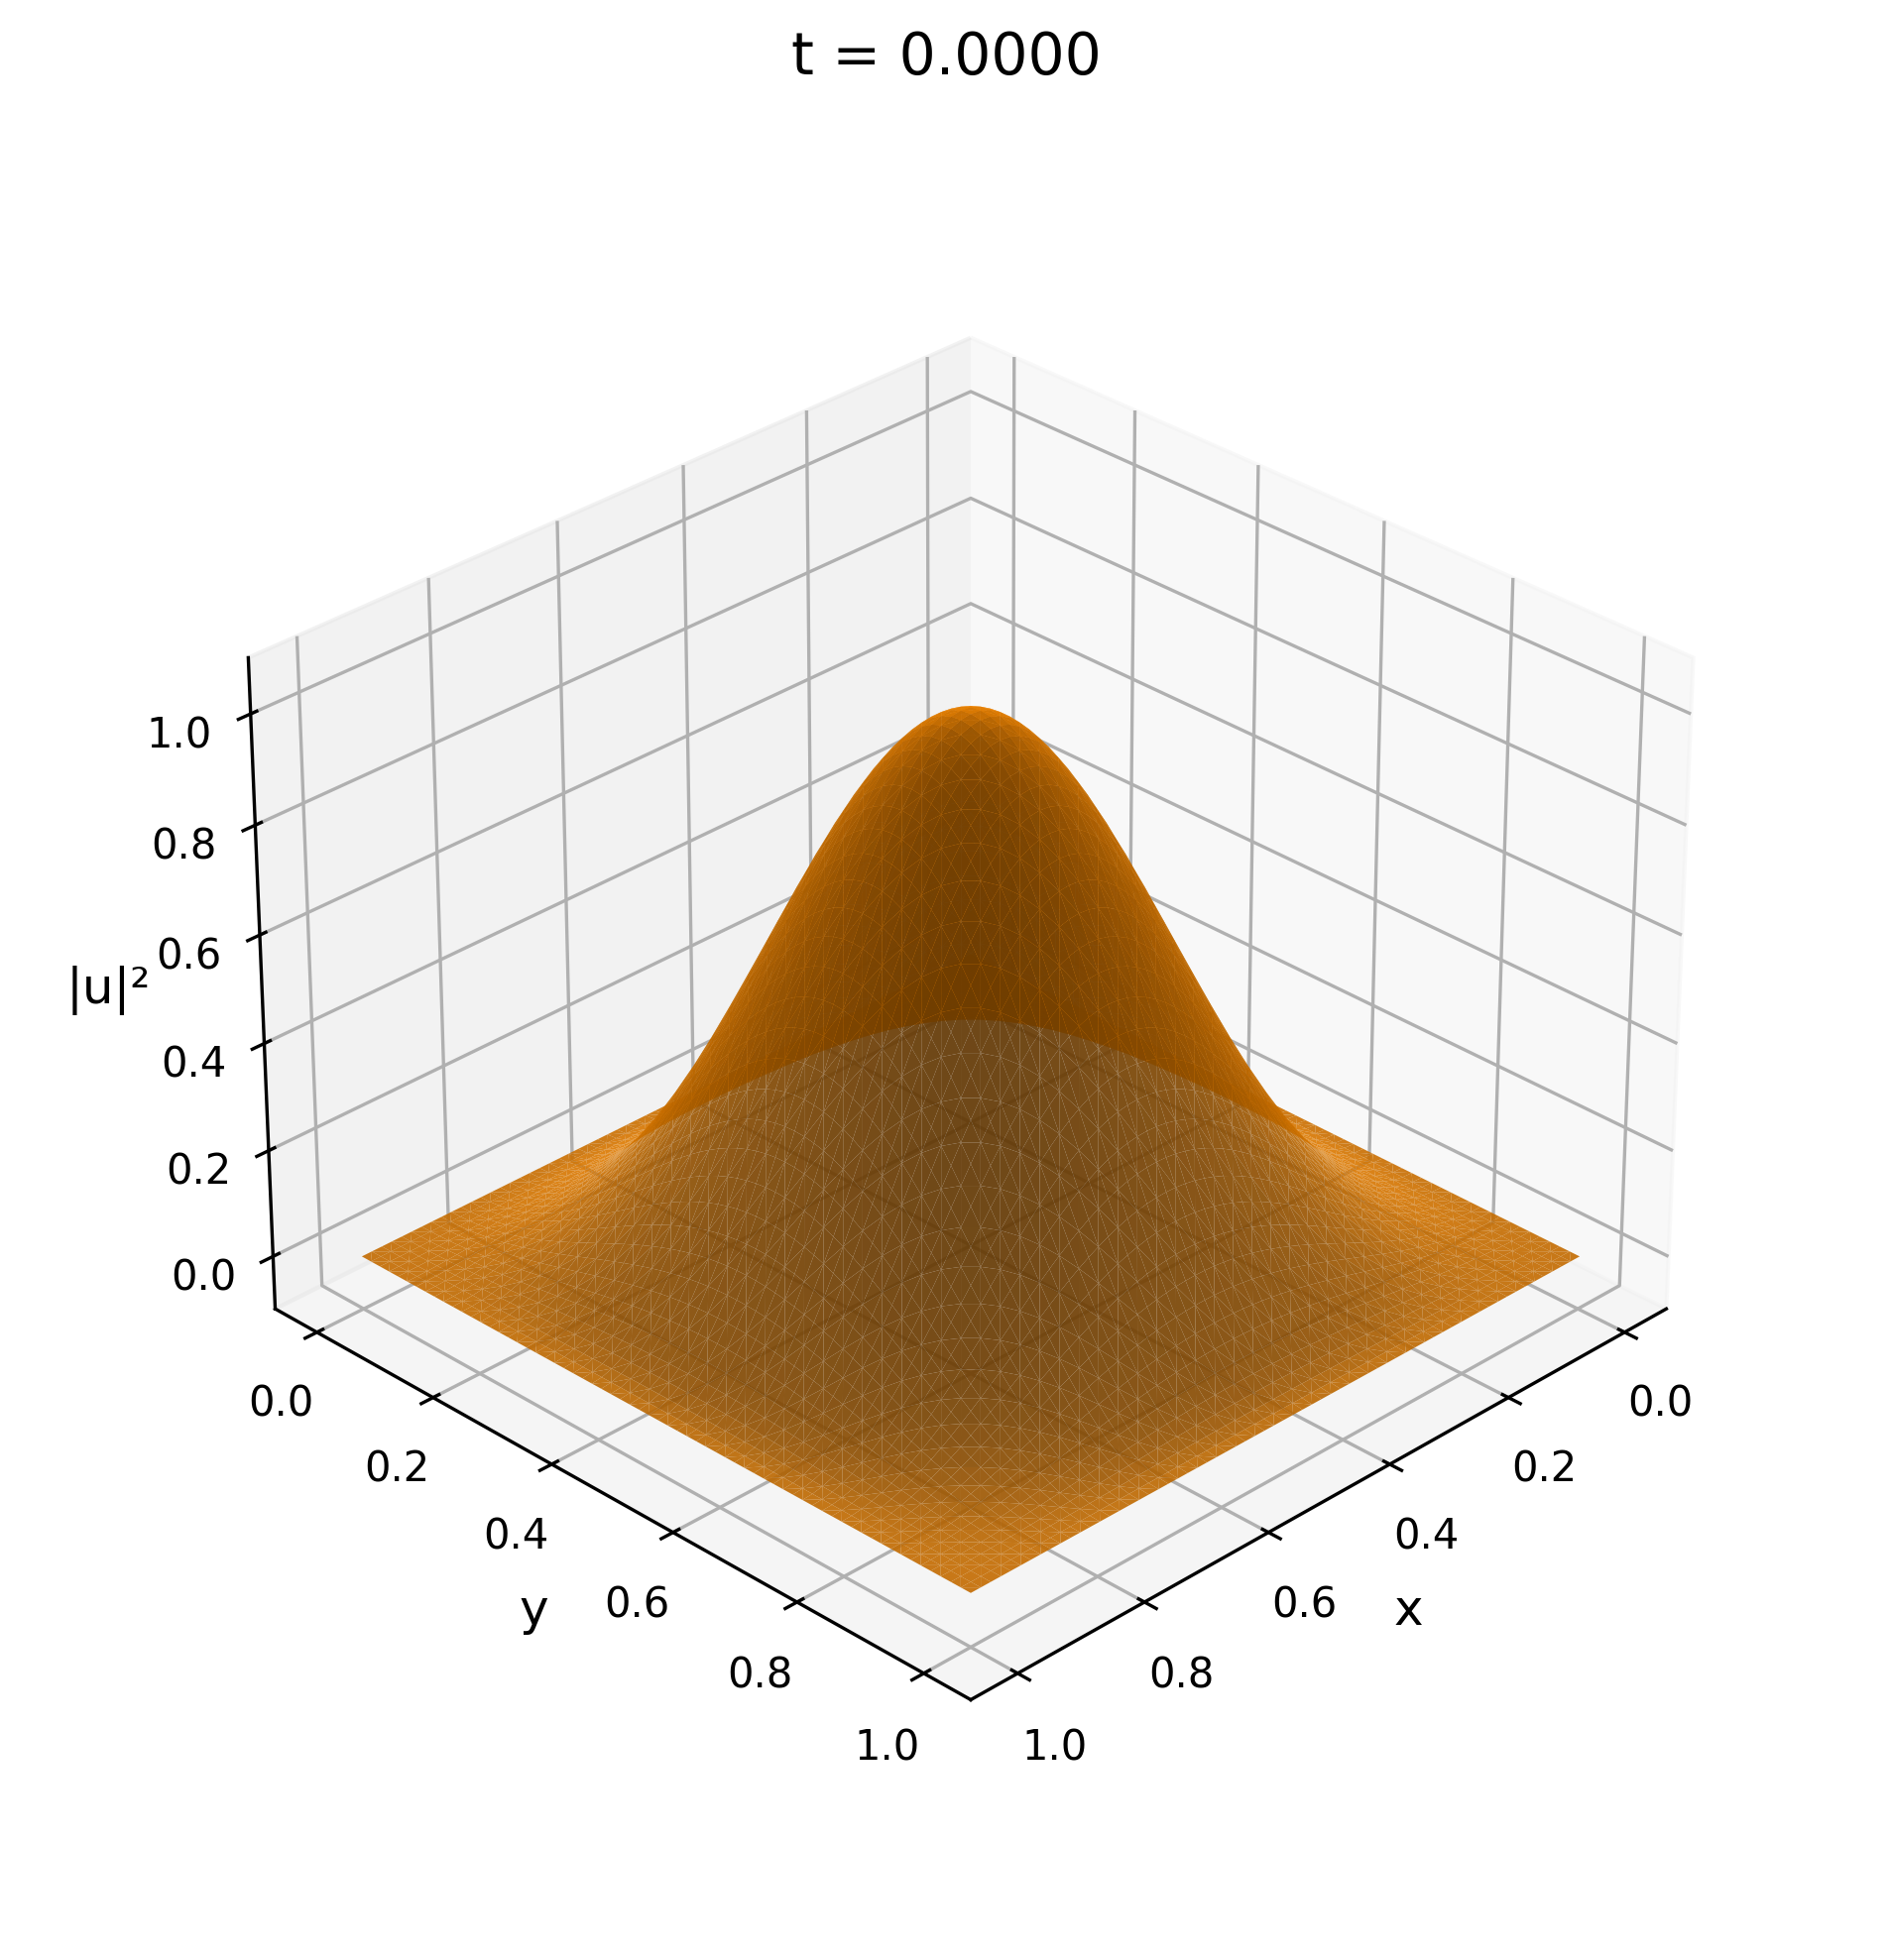
\includegraphics[width=0.7\textwidth]{figures/initial_state_3d.png}
  \caption{Initial State}
  \label{fig:initial_state}
\end{figure}

\subsubsection*{FEM Solution}

We use the variational formulation of the Schrödinger equation derived above, by setting $V(x,t) = 0$ we obtain the weak formulation of the free Schrödinger equation.

We summarize the parameters of the problem as follows:

\begin{itemize}
  \item Meshing: Triangular mesh with $64 \times 64$ elements
  \item Elements: P1 Lagrange elements
  \item Time step size: $\Delta t = 0.00001$
  % \item Boundary conditions: $u = 0$ on $\partial \Omega$
  % \item Initial condition: $u_0(x,y) = \sin(\pi x)\sin(\pi y)$
  % \item Potential: $V(x,t) = 0$
  % \item Exact solution: $u(x,y,t) = \sin(\pi x)\sin(\pi y) e^{-i 2\pi^2 t}$
\end{itemize}

The evolution of the solution for different time steps is shown in Figure \ref{fig:free_solution_evolution}.


\begin{figure}[h]
  \centering
  \begin{subfigure}[b]{0.3\textwidth}
    \centering
    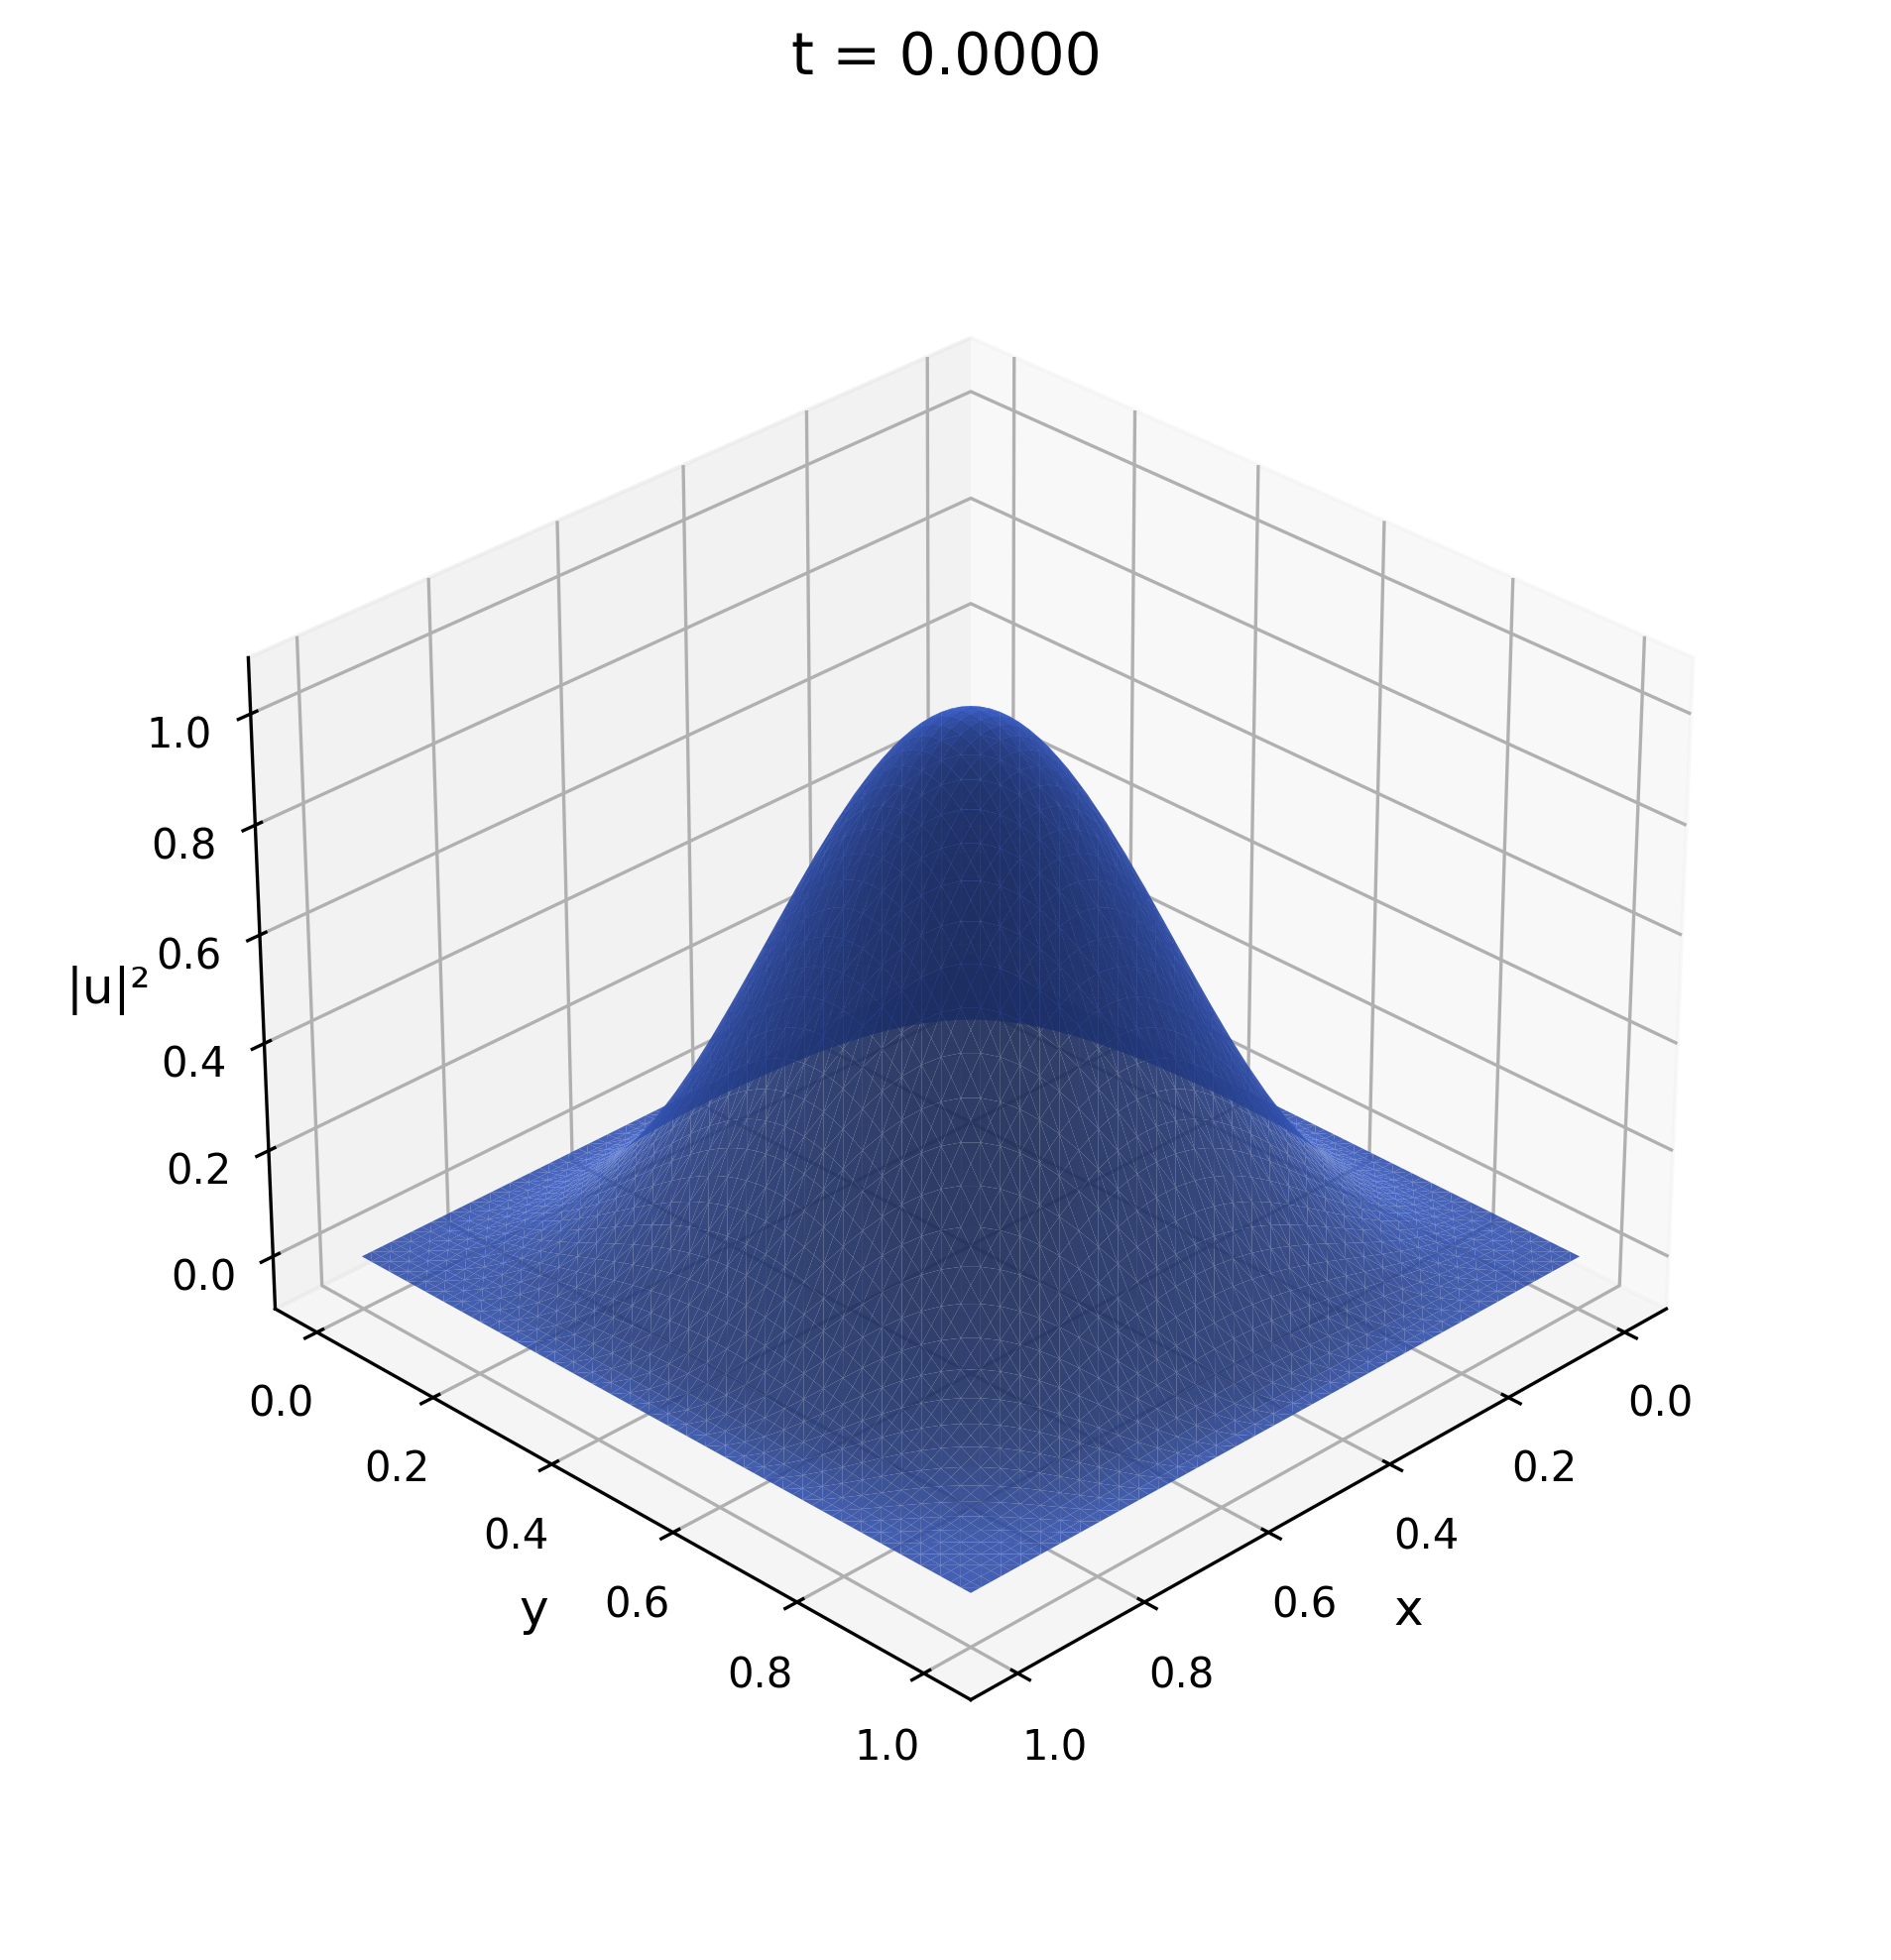
\includegraphics[width=\textwidth, trim=0cm 0cm 0cm 1cm, clip]{figures/fem_frame_0000.png}
    \caption{t = 0.0}
  \end{subfigure}
  \hfill
  \begin{subfigure}[b]{0.3\textwidth}
    \centering
    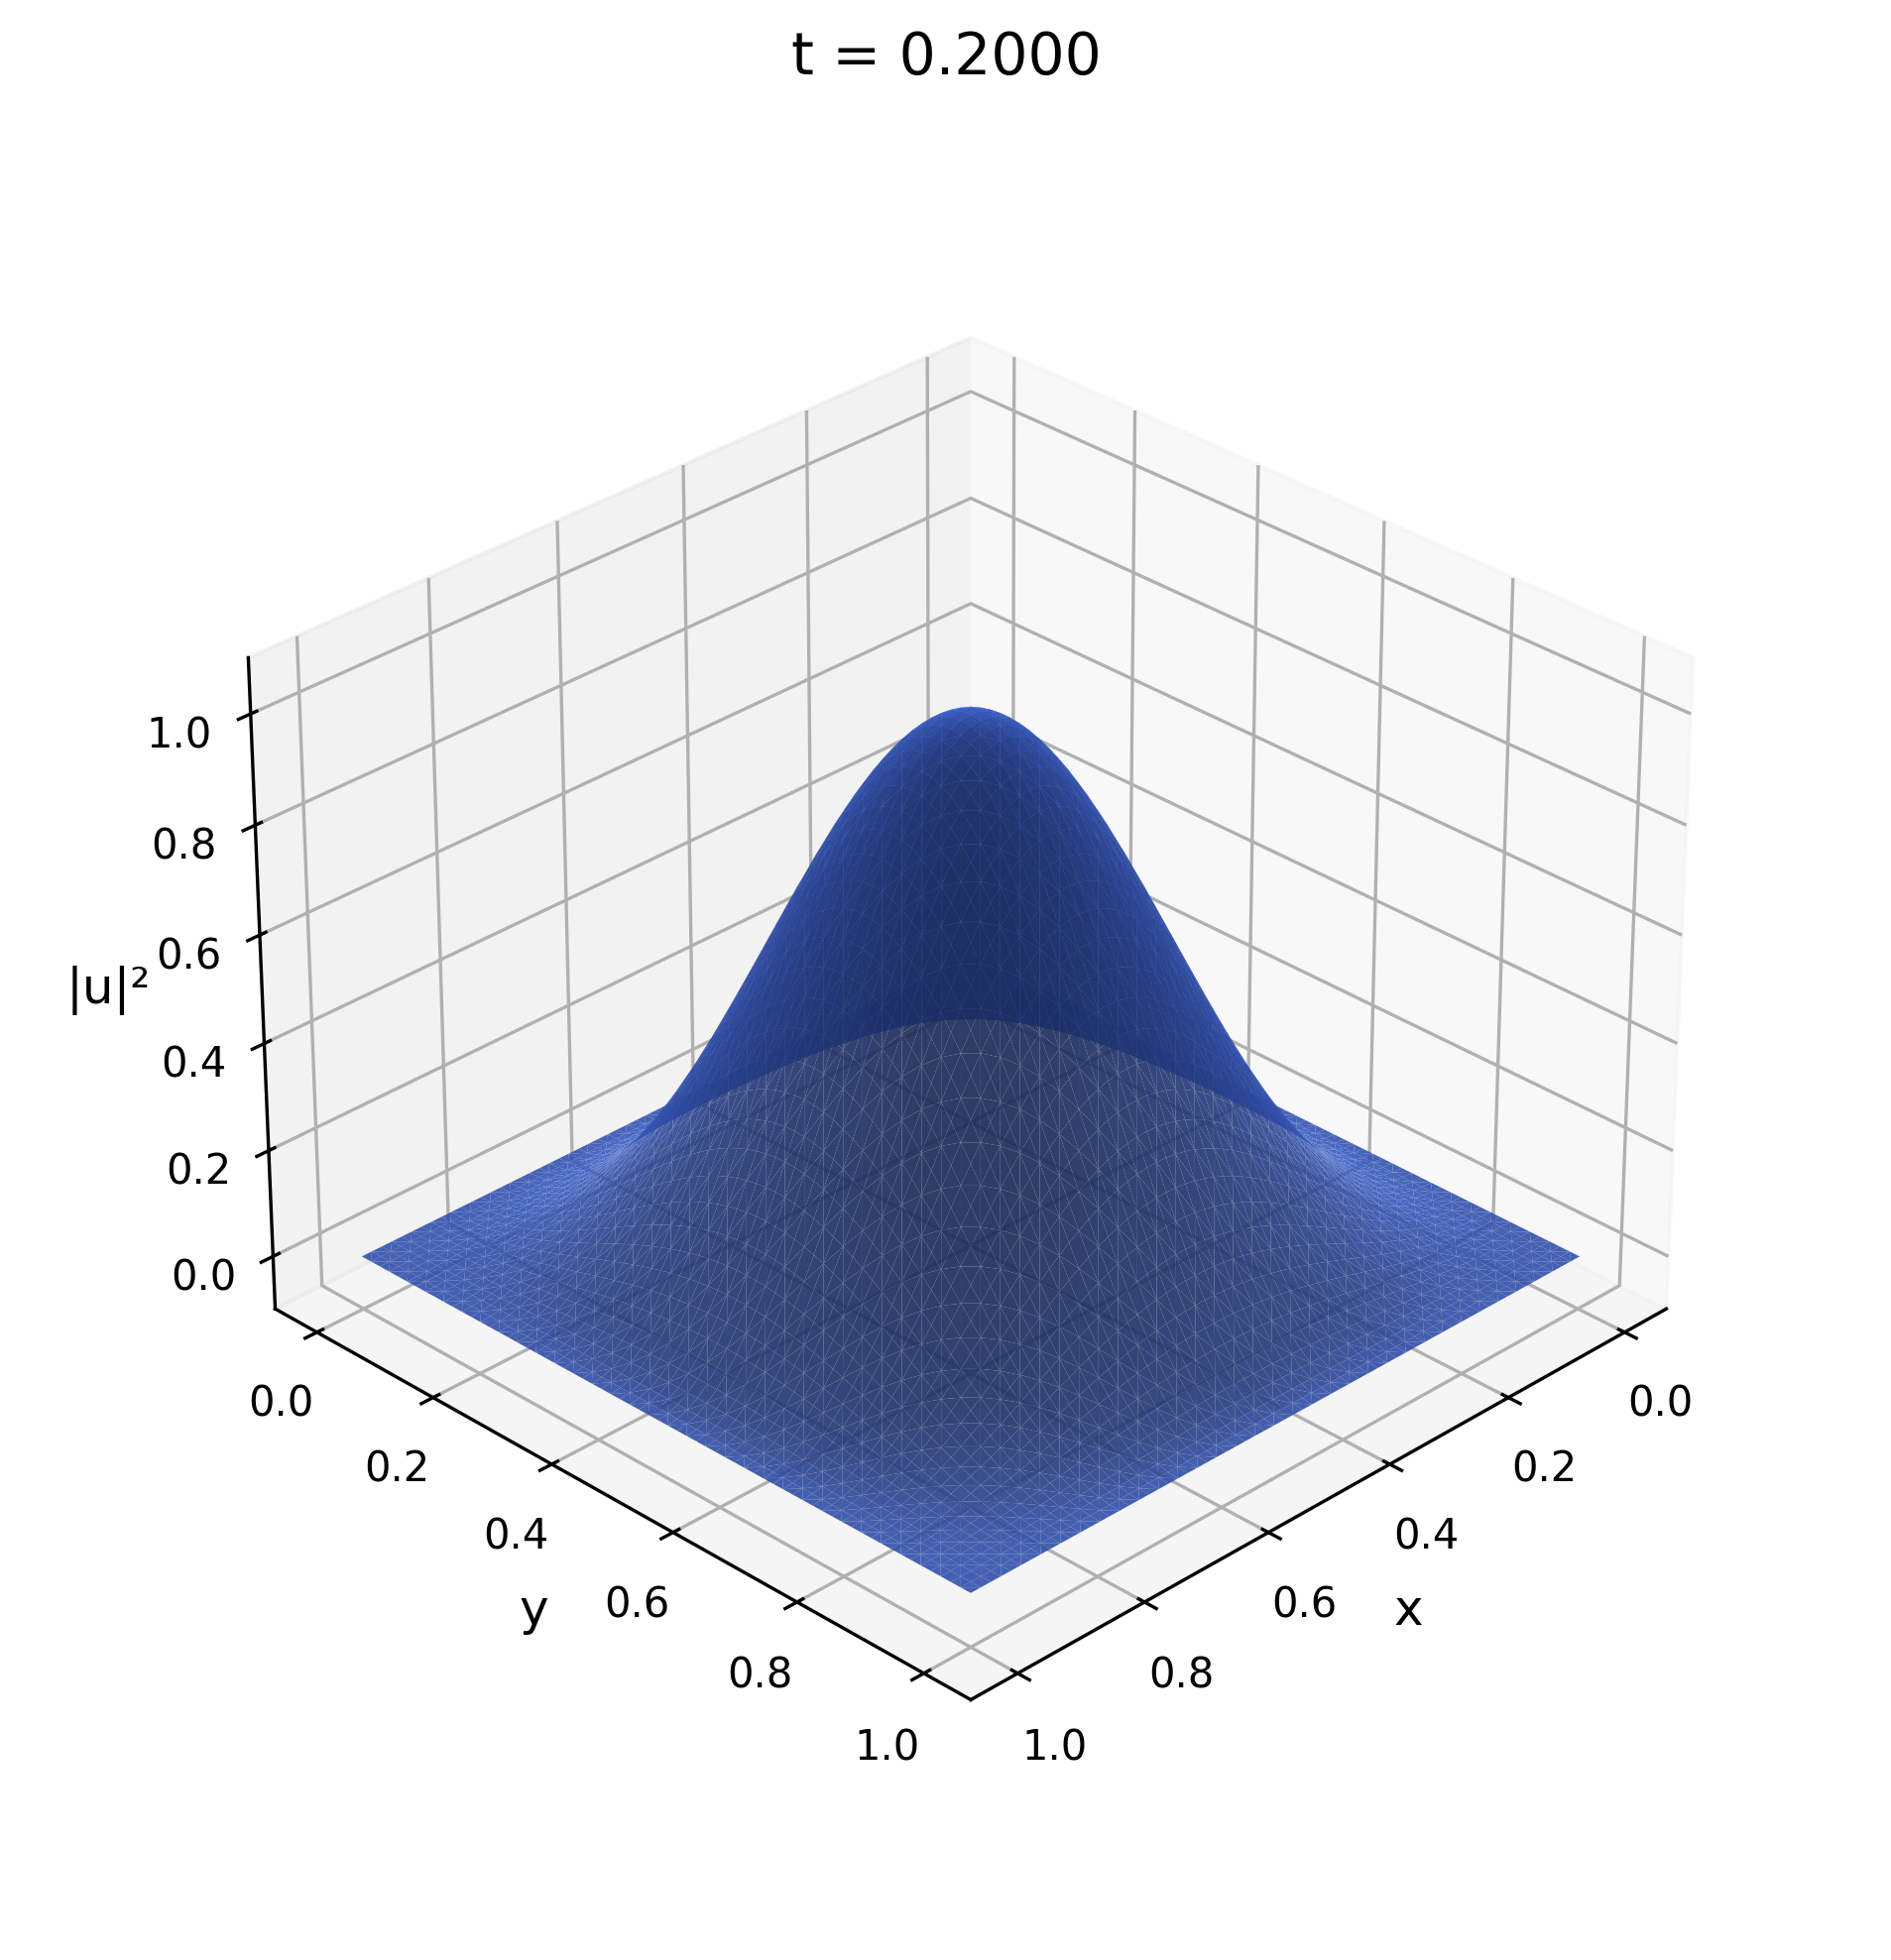
\includegraphics[width=\textwidth, trim=0cm 0cm 0cm 1cm, clip]{figures/fem_frame_0020.png}
    \caption{t = 0.2}
  \end{subfigure}
  \hfill
  \begin{subfigure}[b]{0.3\textwidth}
    \centering
    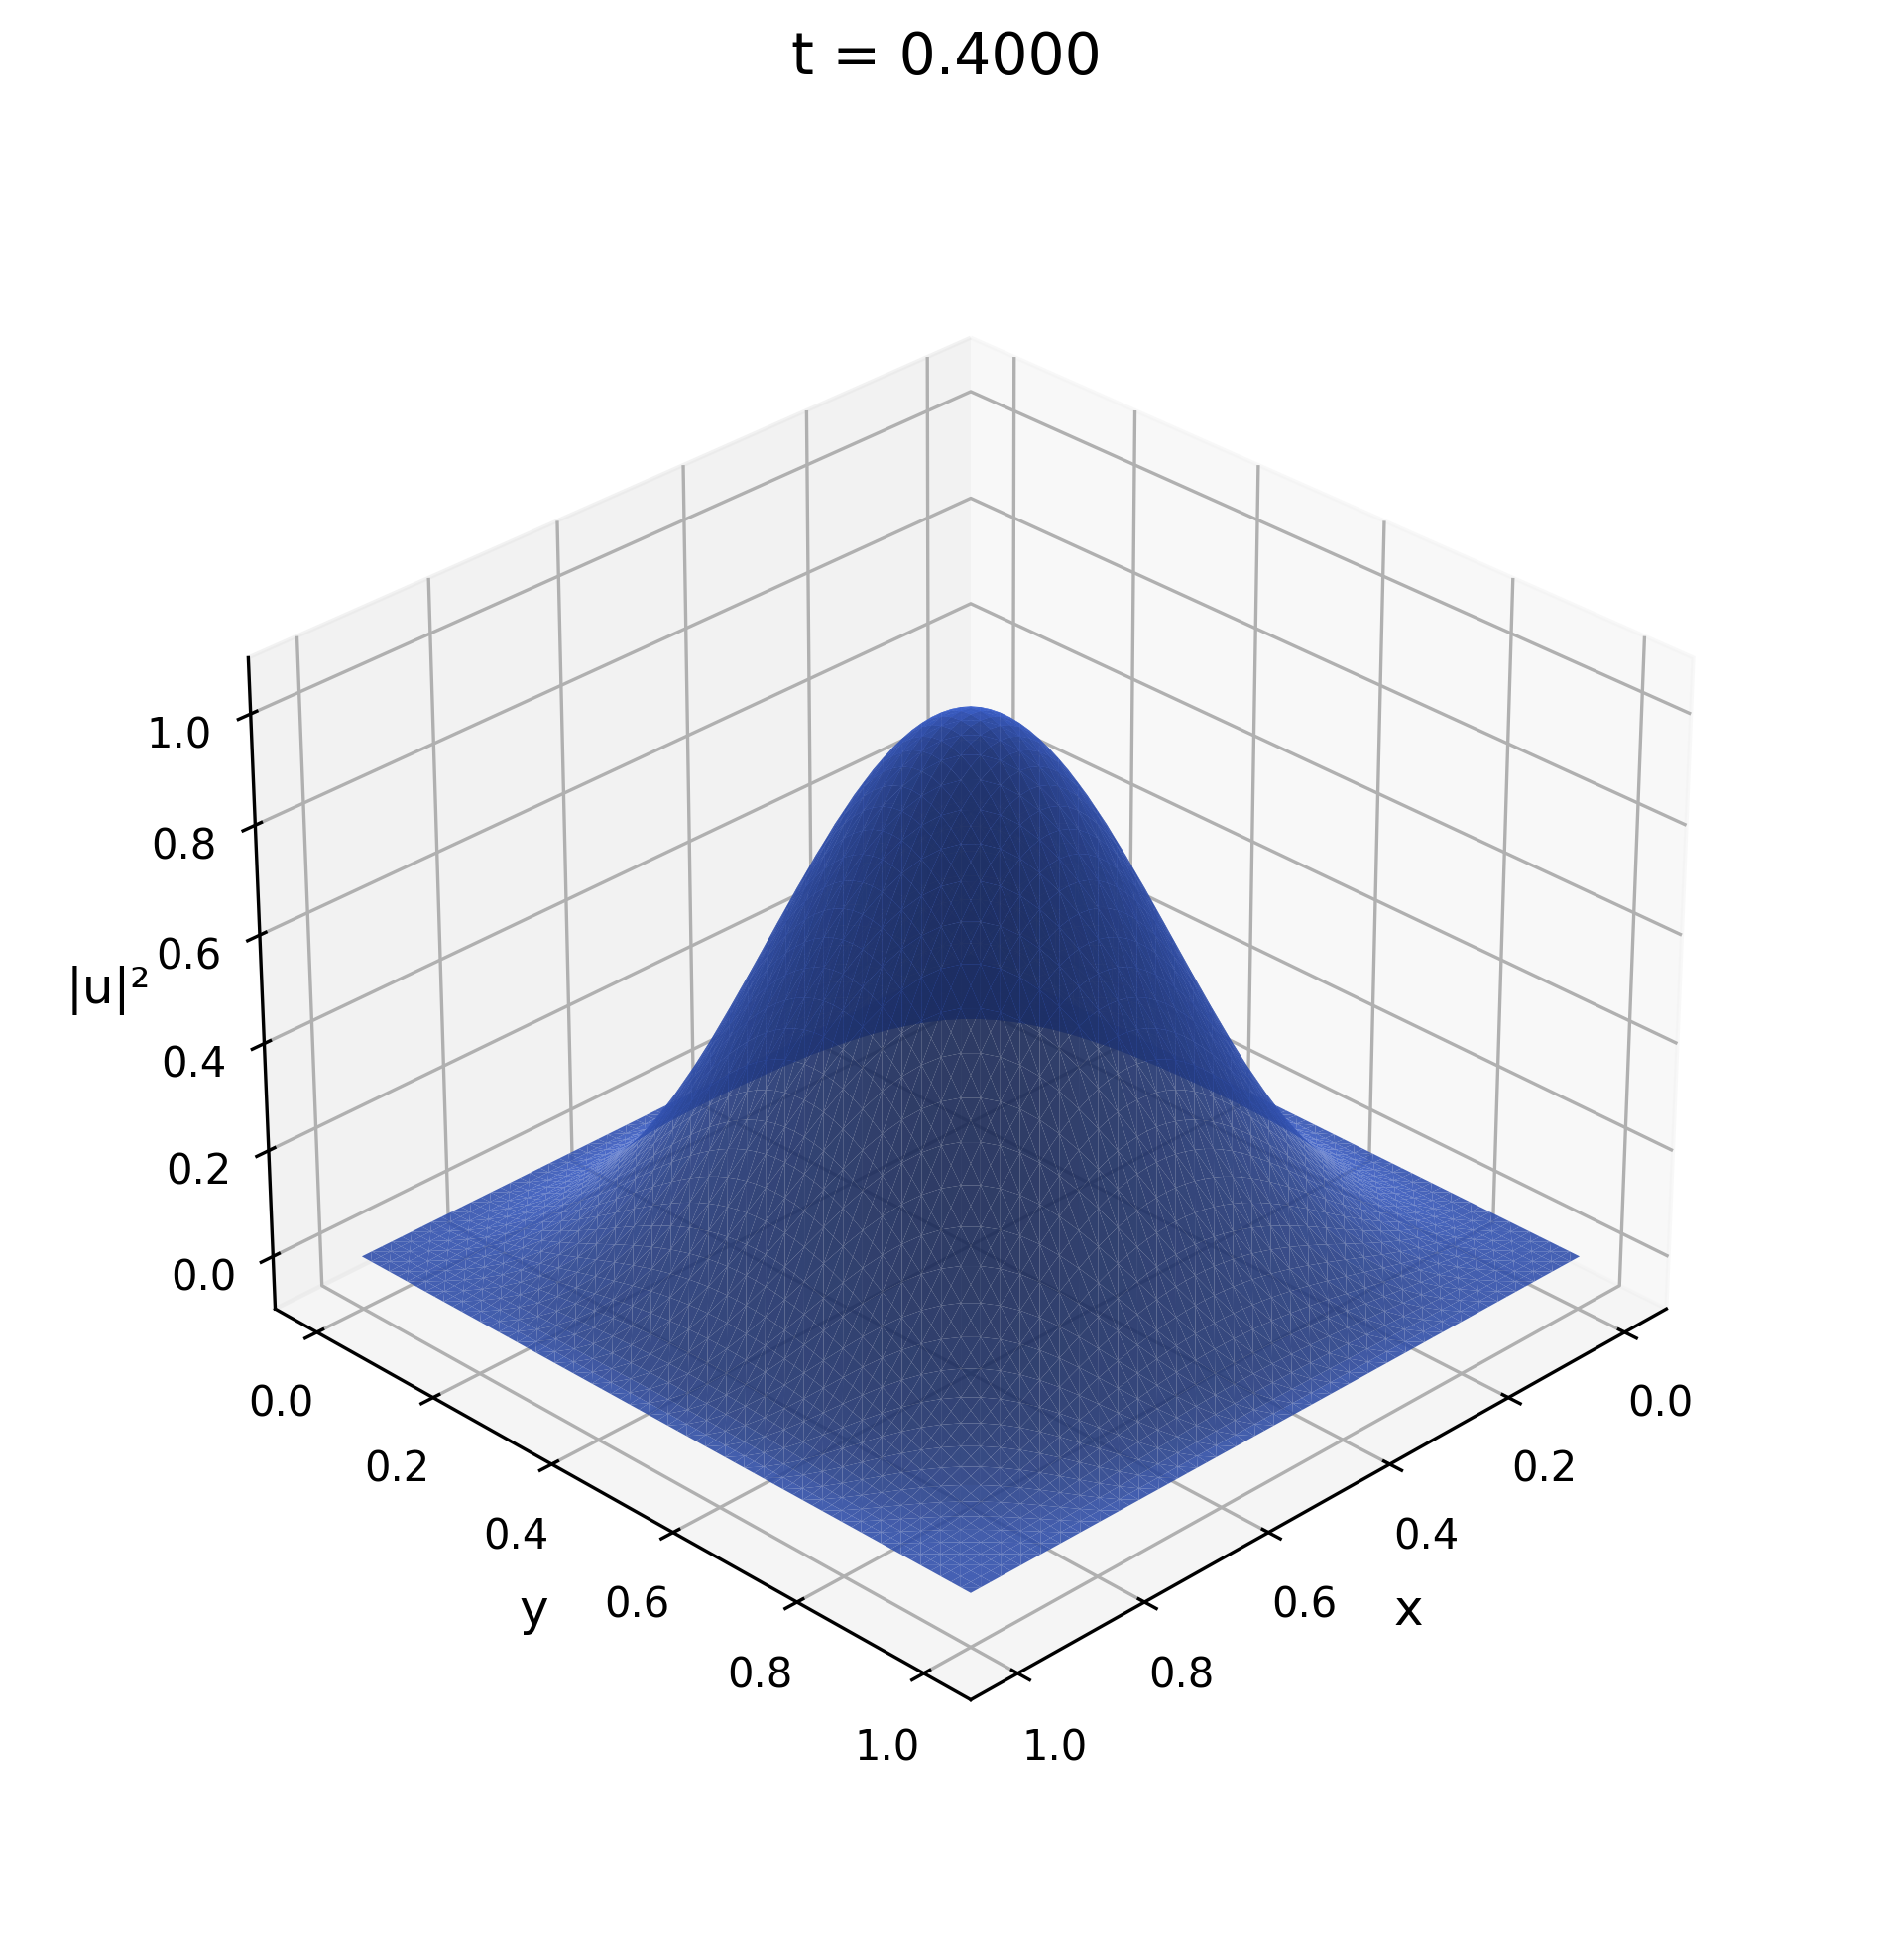
\includegraphics[width=\textwidth, trim=0cm 0cm 0cm 1cm, clip]{figures/fem_frame_0040.png}
    \caption{t = 0.4}
  \end{subfigure}
  
  \vspace{0.5cm}
  
  \begin{subfigure}[b]{0.3\textwidth}
    \centering
    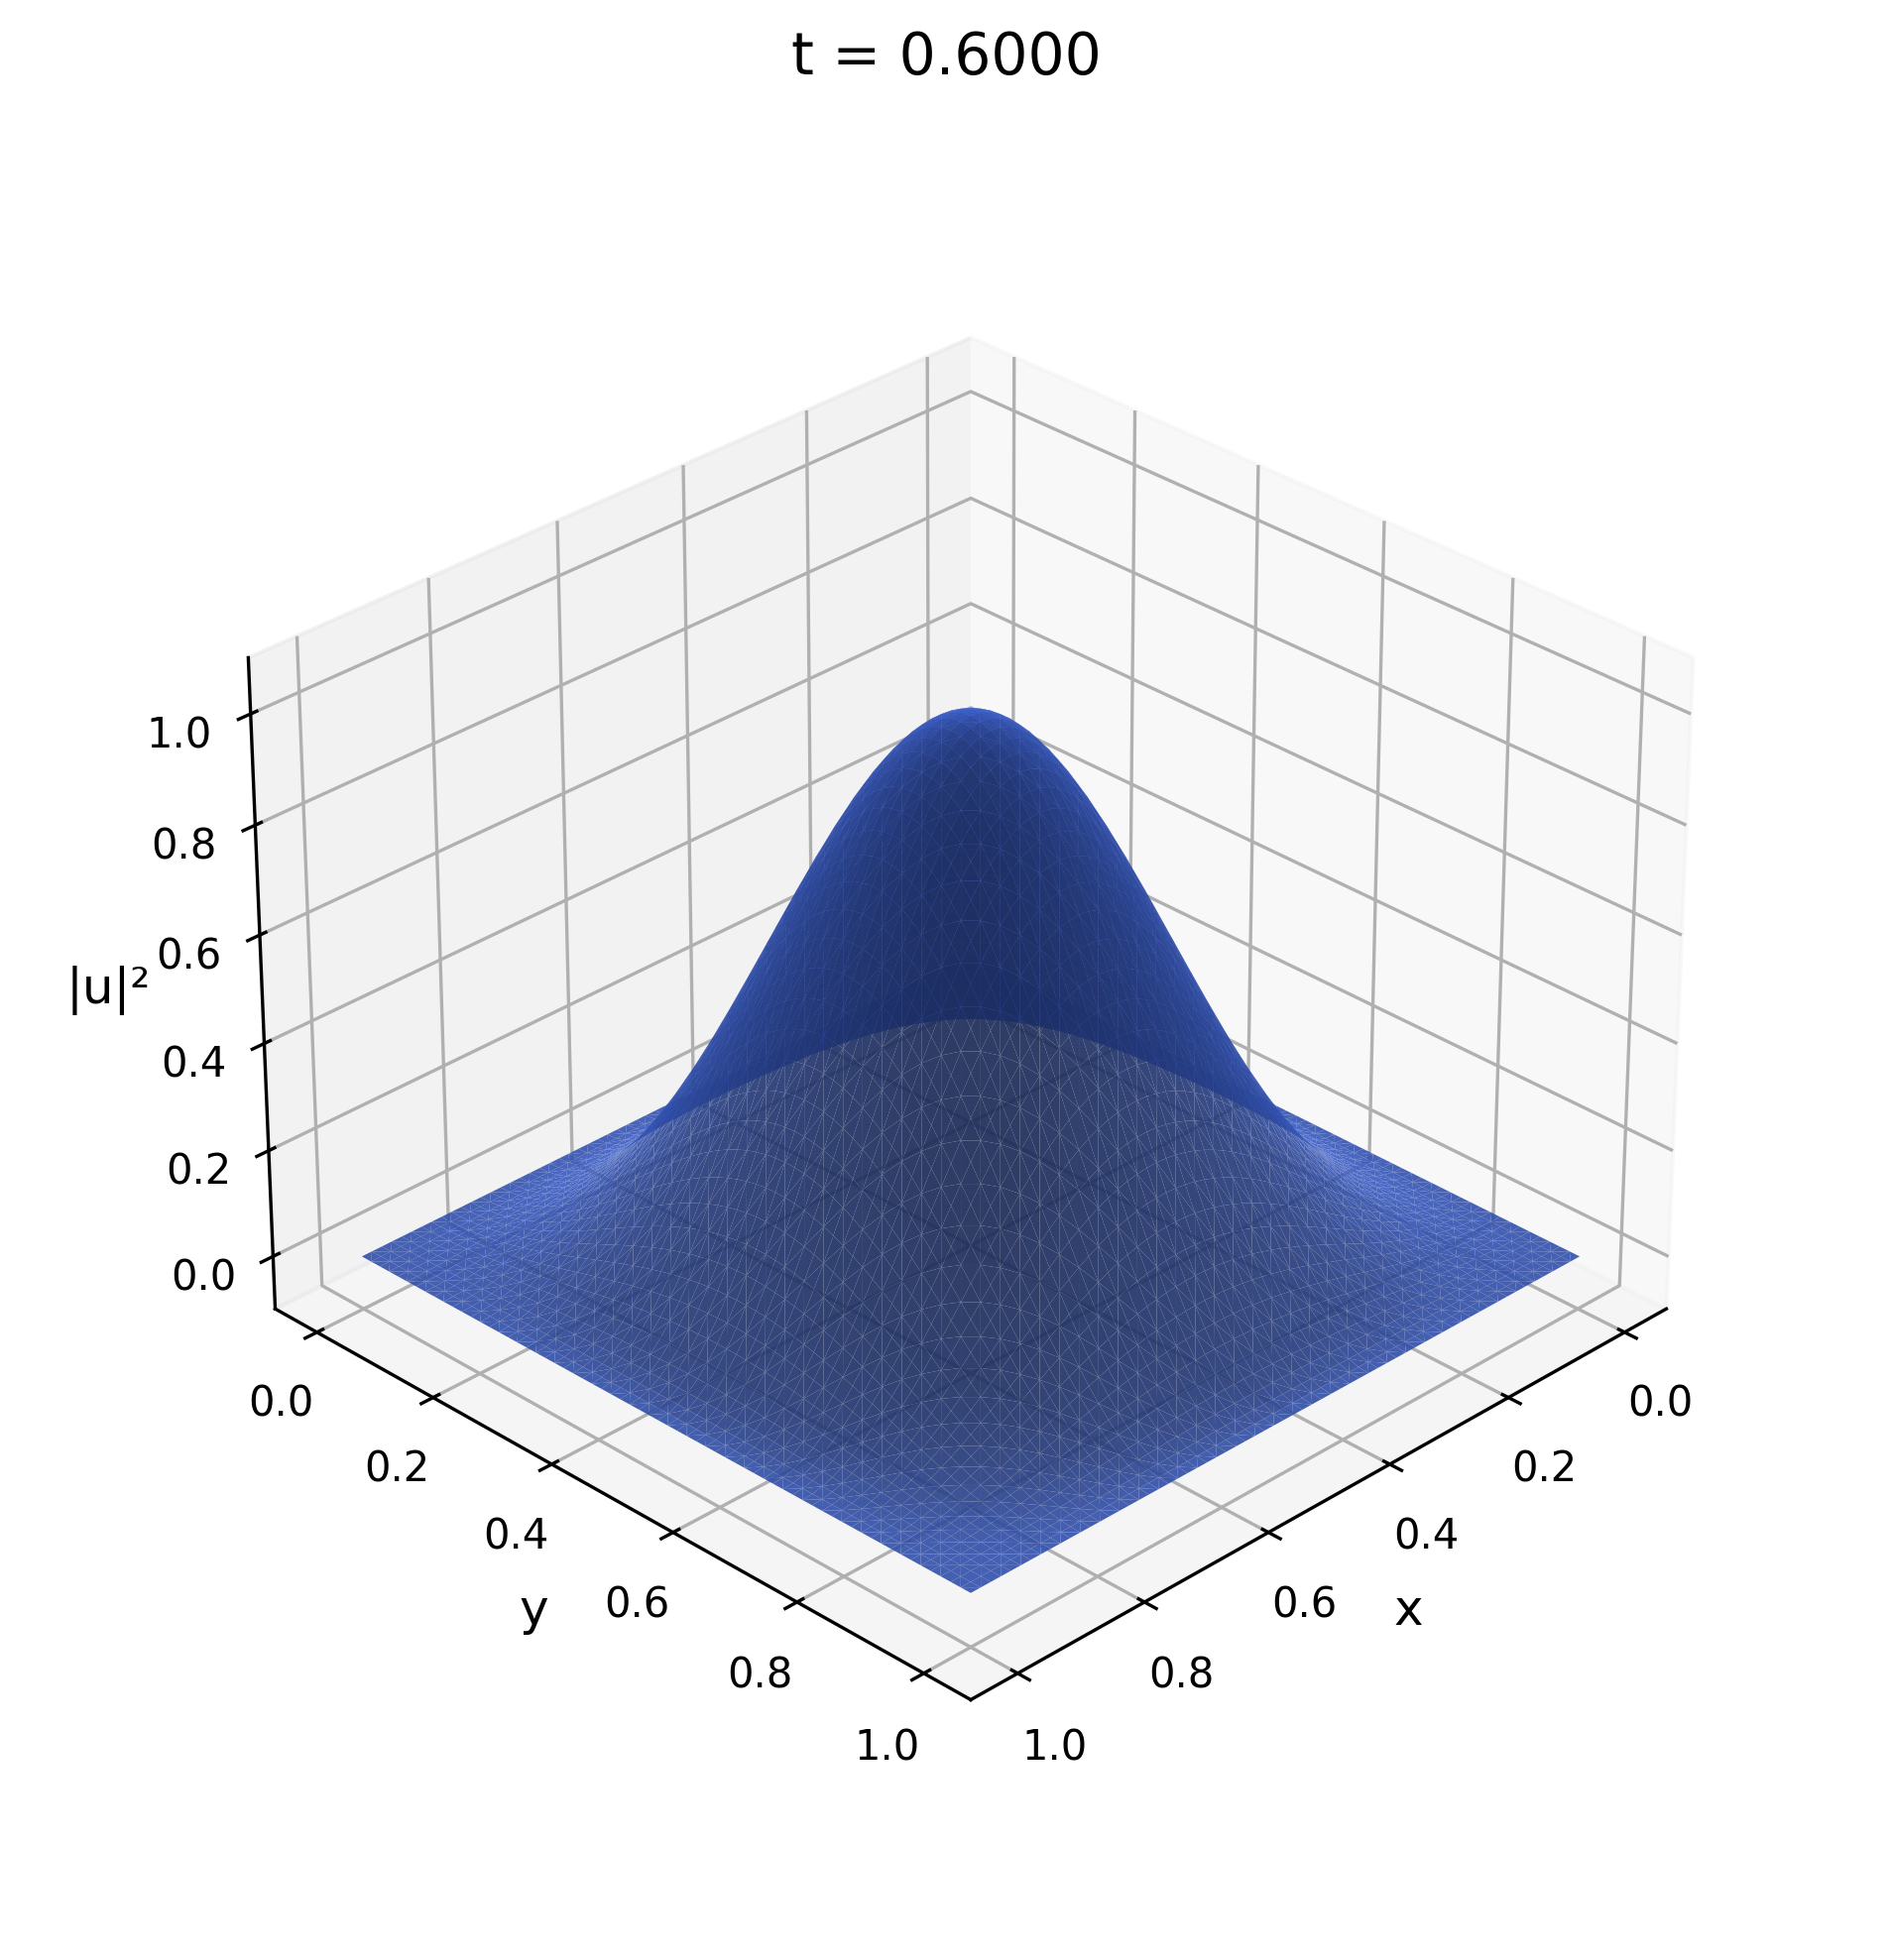
\includegraphics[width=\textwidth, trim=0cm 0cm 0cm 1cm, clip]{figures/fem_frame_0060.png}
    \caption{t = 0.6}
  \end{subfigure}
  \hfill
  \begin{subfigure}[b]{0.3\textwidth}
    \centering
    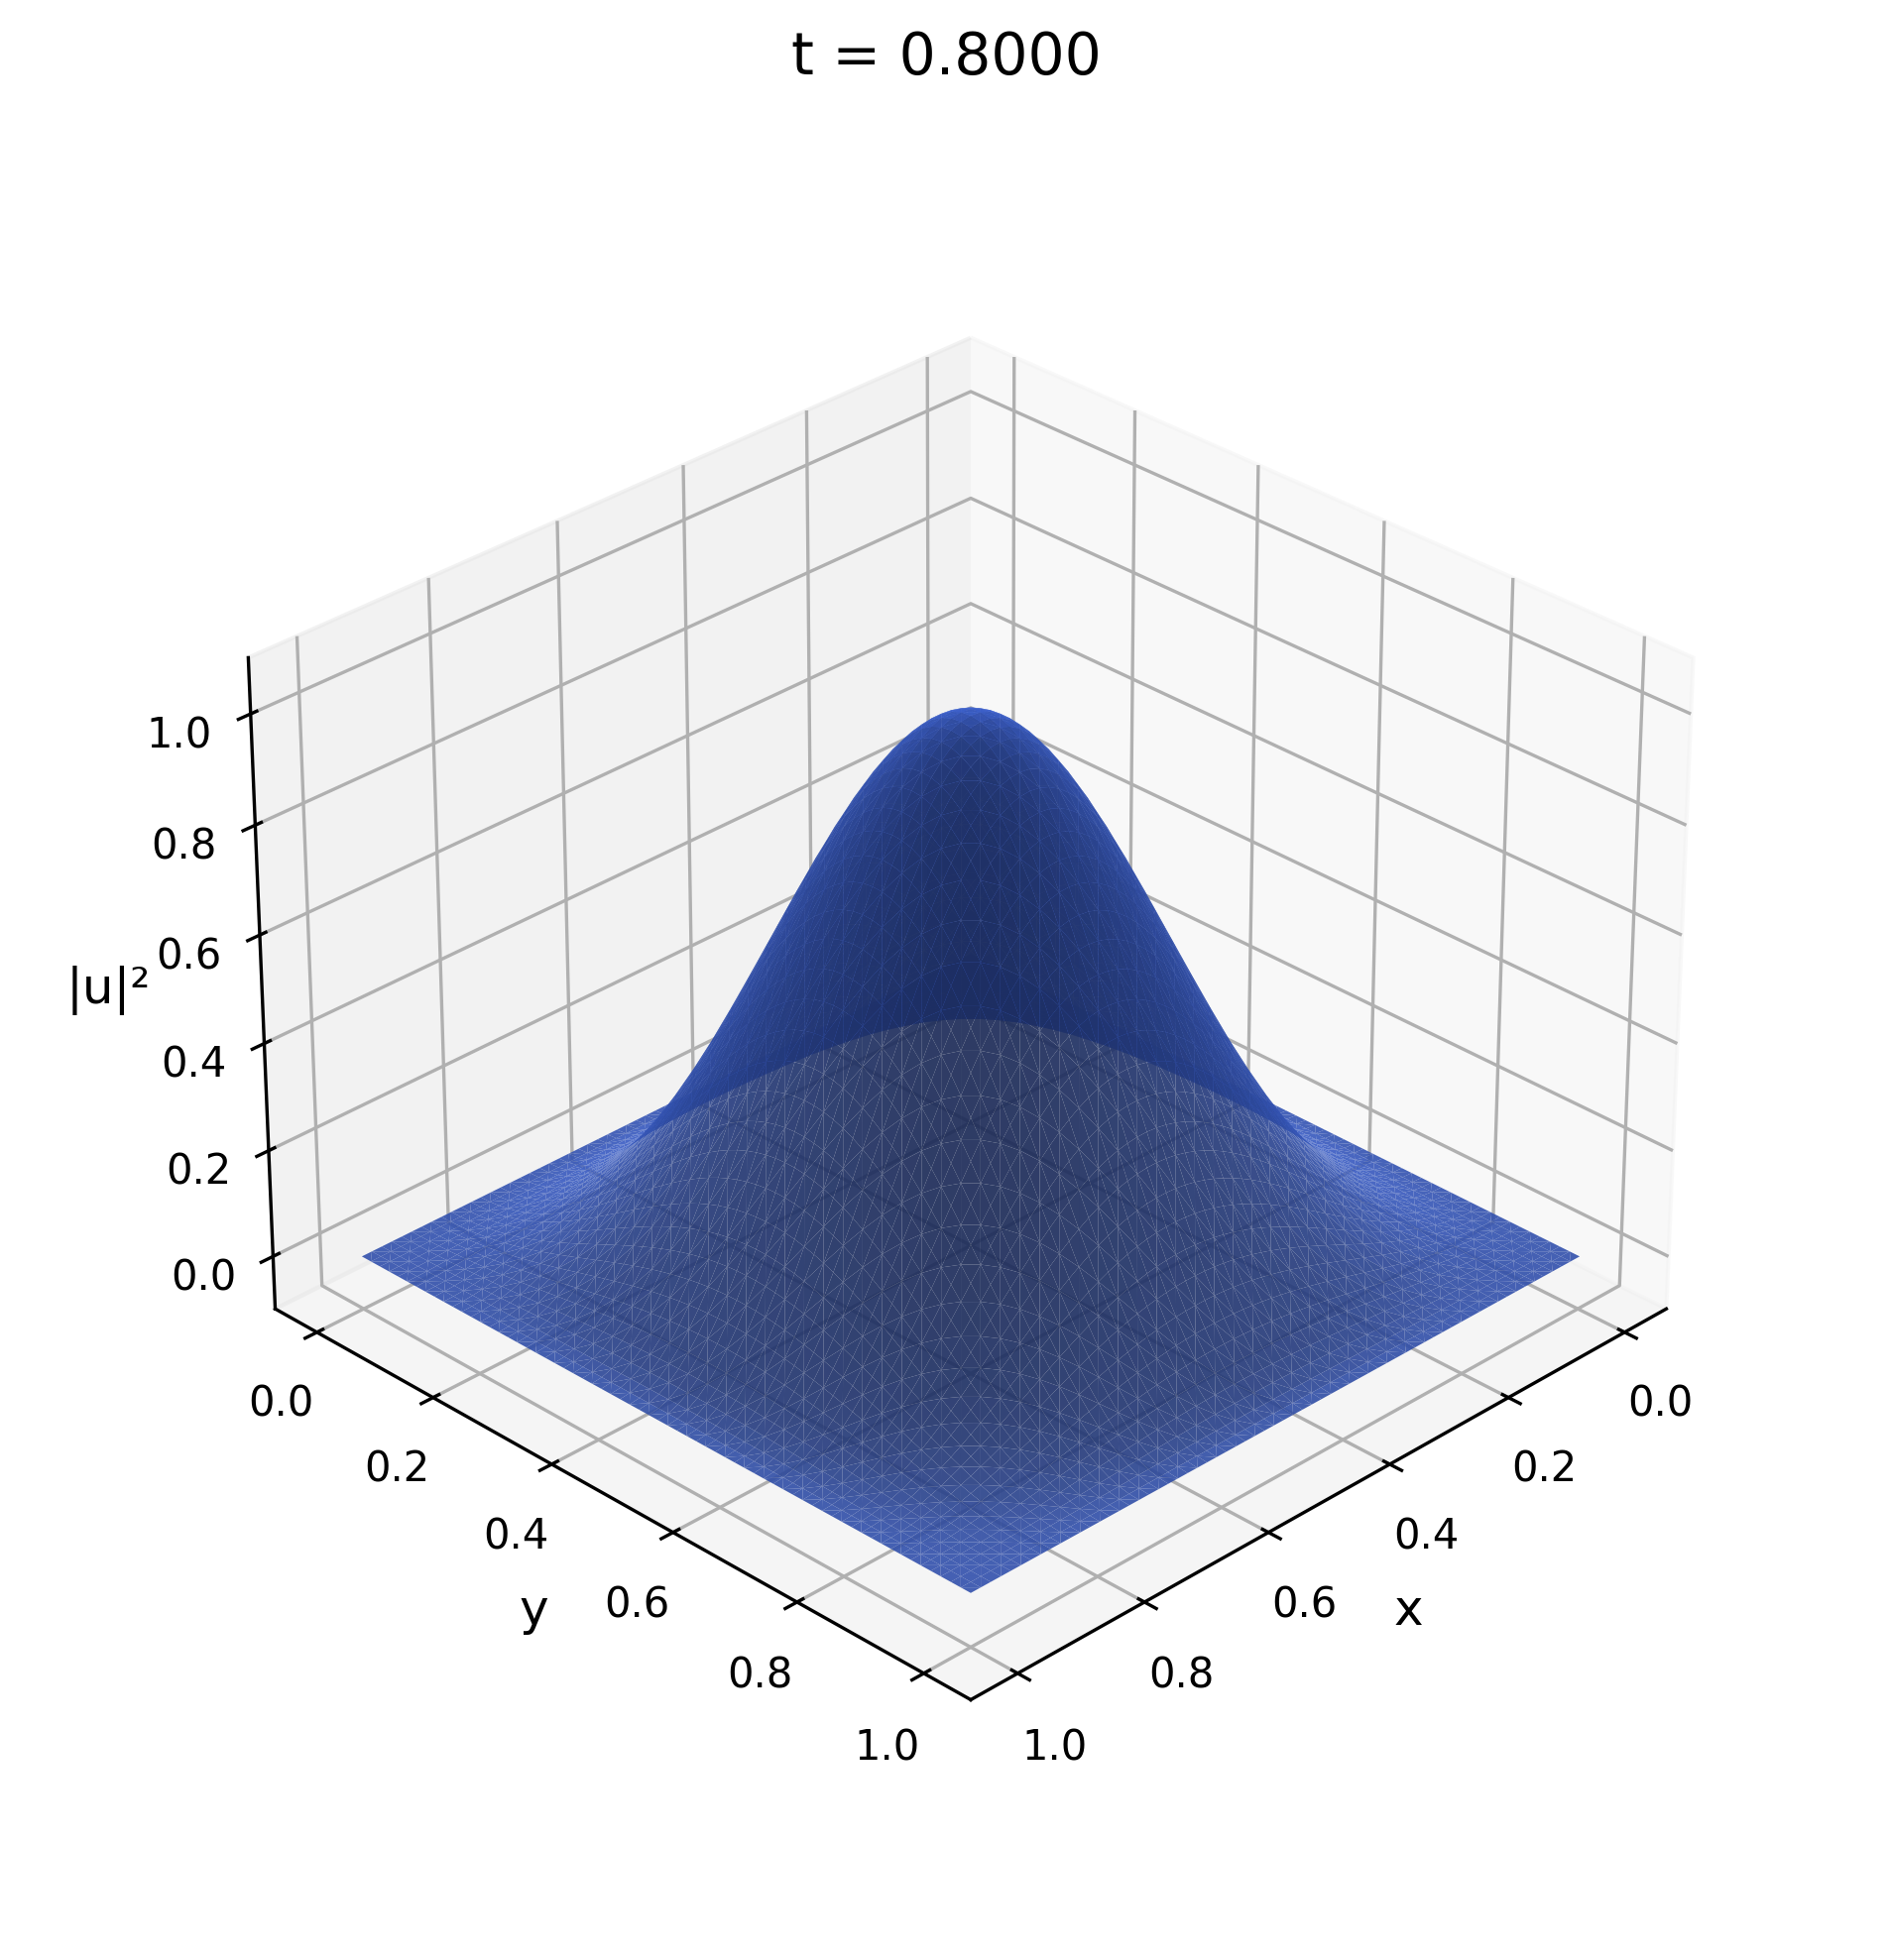
\includegraphics[width=\textwidth, trim=0cm 0cm 0cm 1cm, clip]{figures/fem_frame_0080.png}
    \caption{t = 0.8}
  \end{subfigure}
  \hfill
  \begin{subfigure}[b]{0.3\textwidth}
    \centering
    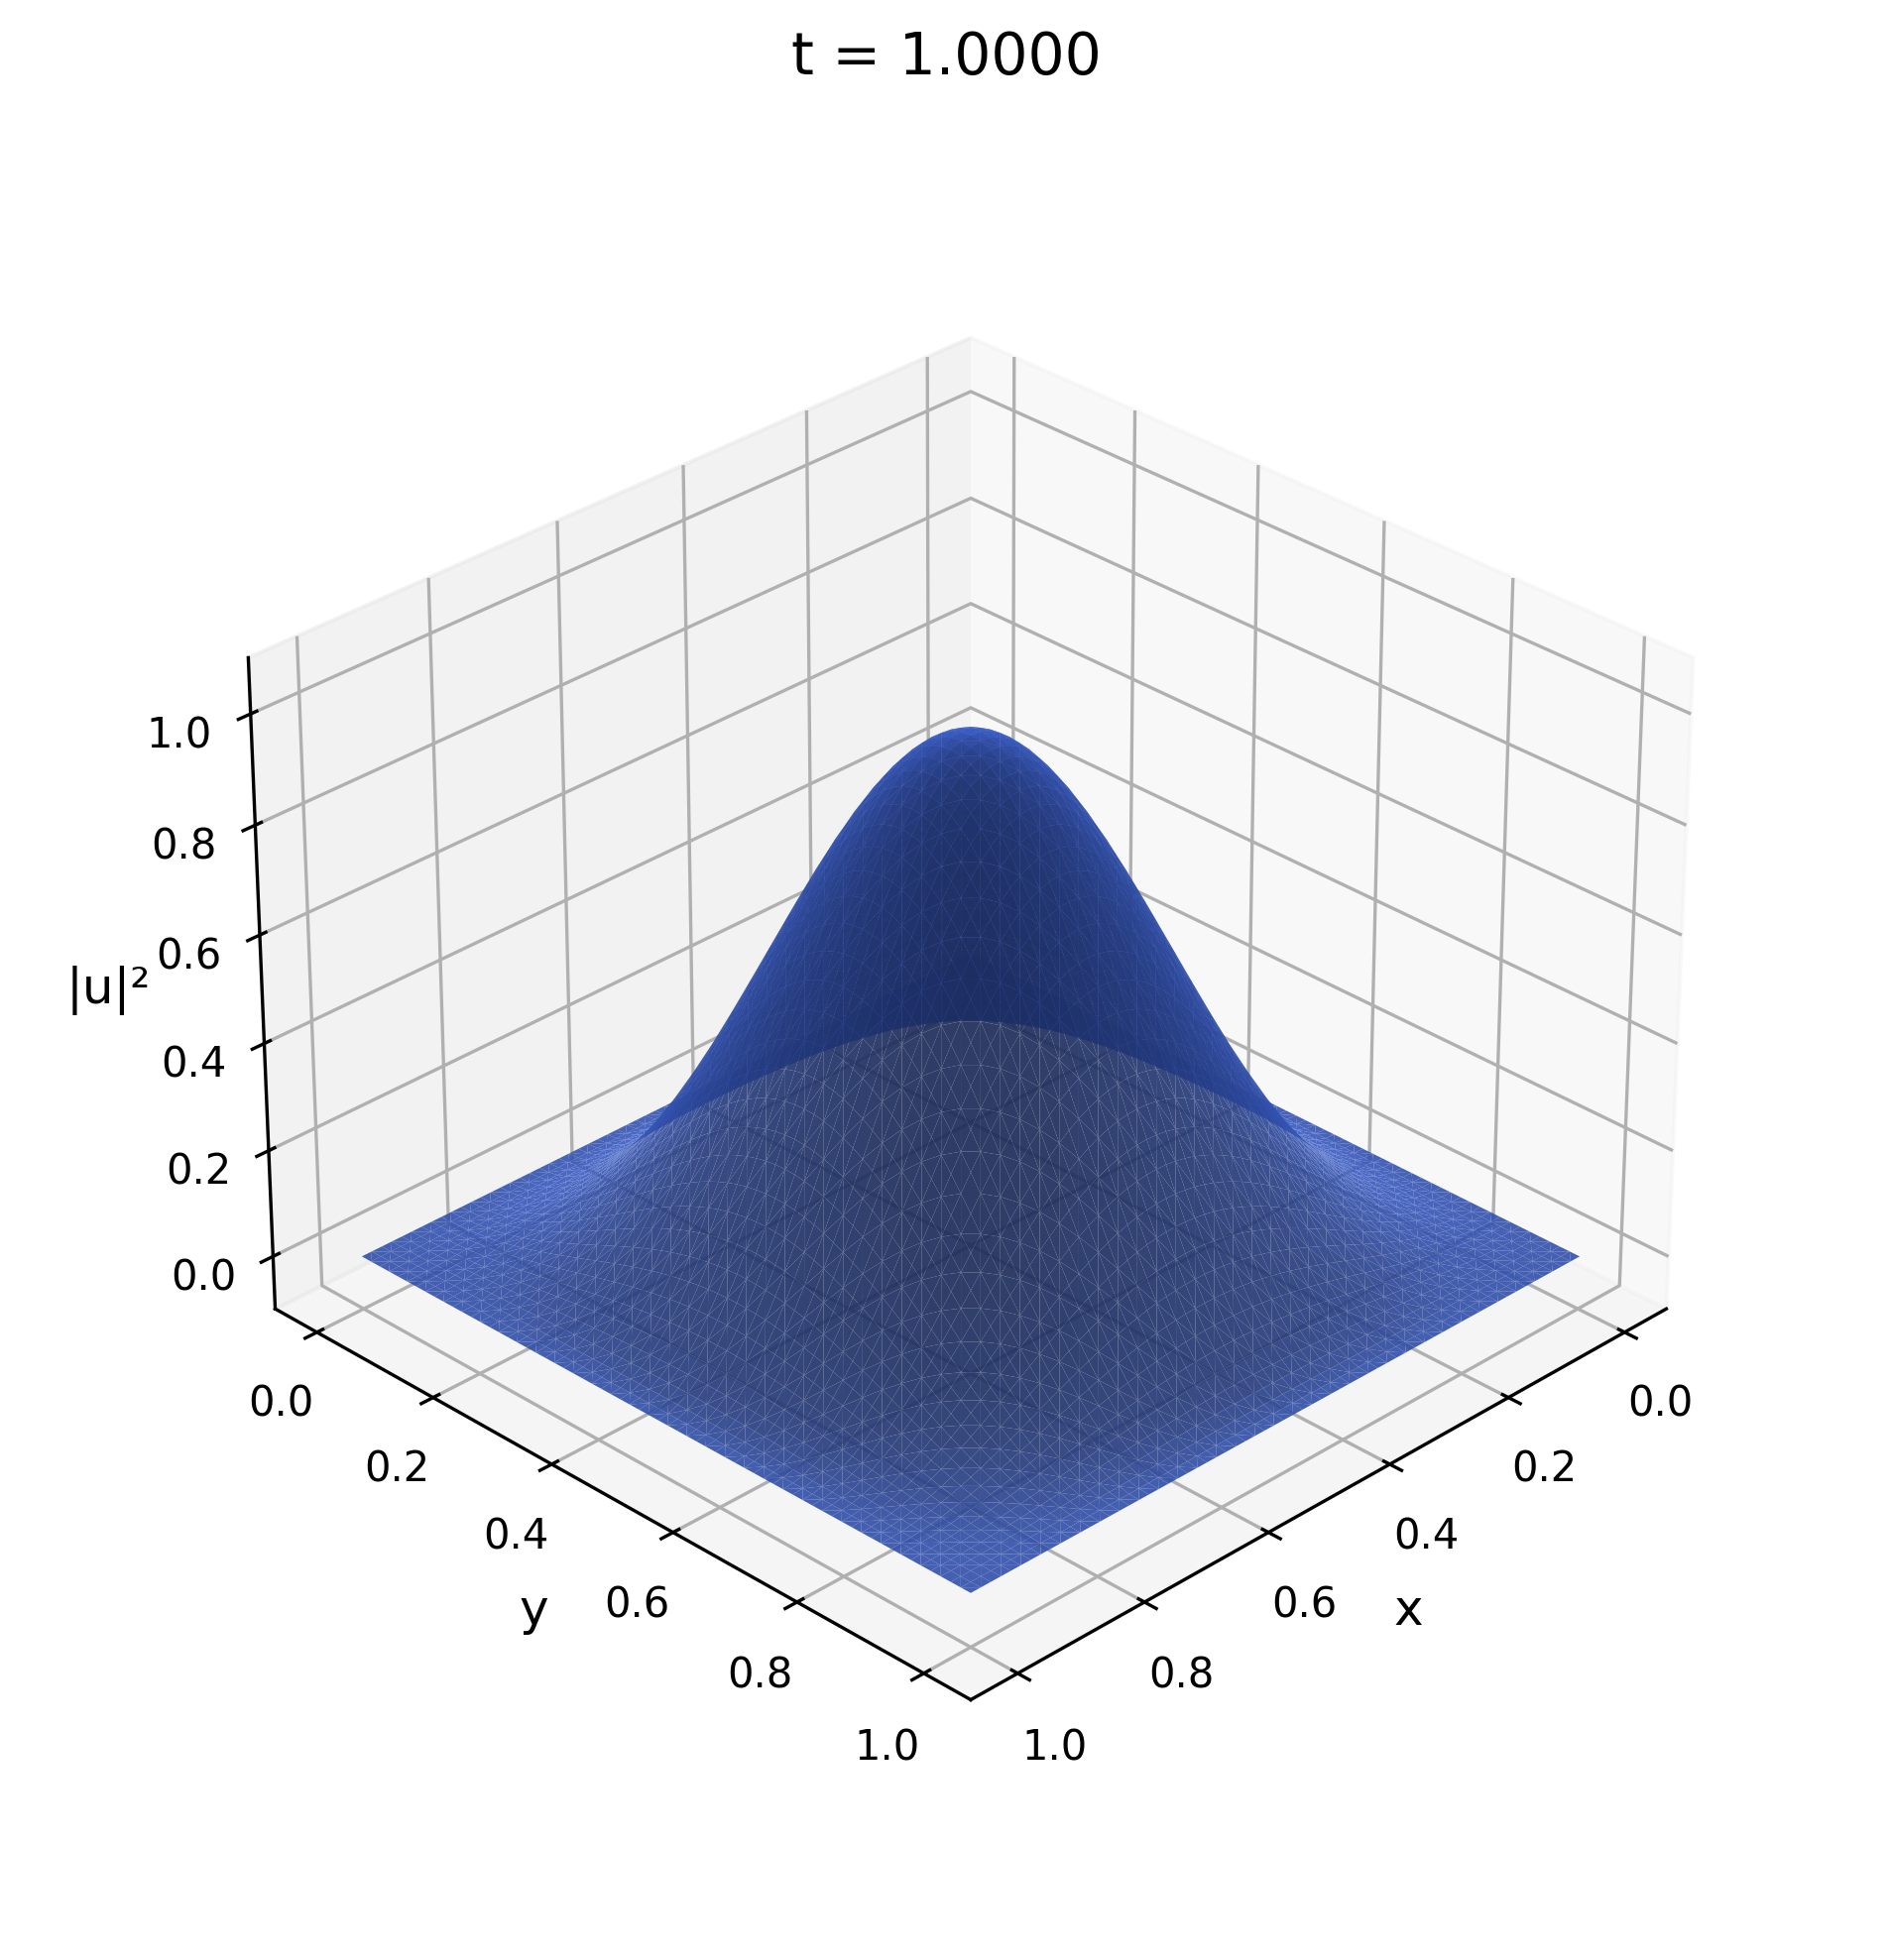
\includegraphics[width=\textwidth, trim=0cm 0cm 0cm 1cm, clip]{figures/fem_frame_0100.png}
    \caption{t = 1.0}
  \end{subfigure}
  \caption{Time evolution of the solution of the free Schrödinger equation, obtained with the FEM.}
  \label{fig:free_solution_evolution}
\end{figure}

We can see that the solution is a standing wave, which is expected for the free Schrödinger equation. (stimmt das?)

\subsubsection*{Error Analysis}

The approximation error of the numerical solution has two components: 
\begin{itemize}
  \item the discretization error due to the finite element method,
  \item the time-stepping error due to the backward Euler method.
\end{itemize}
We define the error vector $e_h^{(t)}$ as the difference between the numerical solution $u_h^{(t)}$ and the exact solution $u^{(t)}$ at each time step:
\[
e_h^{(t)} = u_h^{(t)} - u^{(t)}.
\]
Figure \ref{fig:2d_error_analysis} shows the $L^2$ norm of the error vector over time for different mesh sizes.
From this plot we can see that the error increases linearly with time, which is expected for the backward Euler method.
For finer meshes the error is smaller, as the FEM discretization error decreases and the time error remains. 
This gets perfectly visible for the refinements $n=64, 128, 256$ where the error behaves almost the same for all resolutions.

Figure \ref{fig:2d_error_analysis_2} shows the $L^2$ norm of the error vector over mesh sizes for different timesteps.
It also shows a reference line described of order  $\mathcal{O}(h^2)$, which is the expected convergence rate for the FEM with P1 elements.
We see that for coarser meshes the error perfectly meets the slope of the reference line.
Again for the last three refinements $h=1/64, 1/128, 1/256$ the error does not decrease significantly anymore, which indicates again, that the time stepping error dominates the overall error.
It also gets obvious that through error propagation the error increases with time, which is expected for the backward Euler method.

\begin{figure}[h]
  \centering
  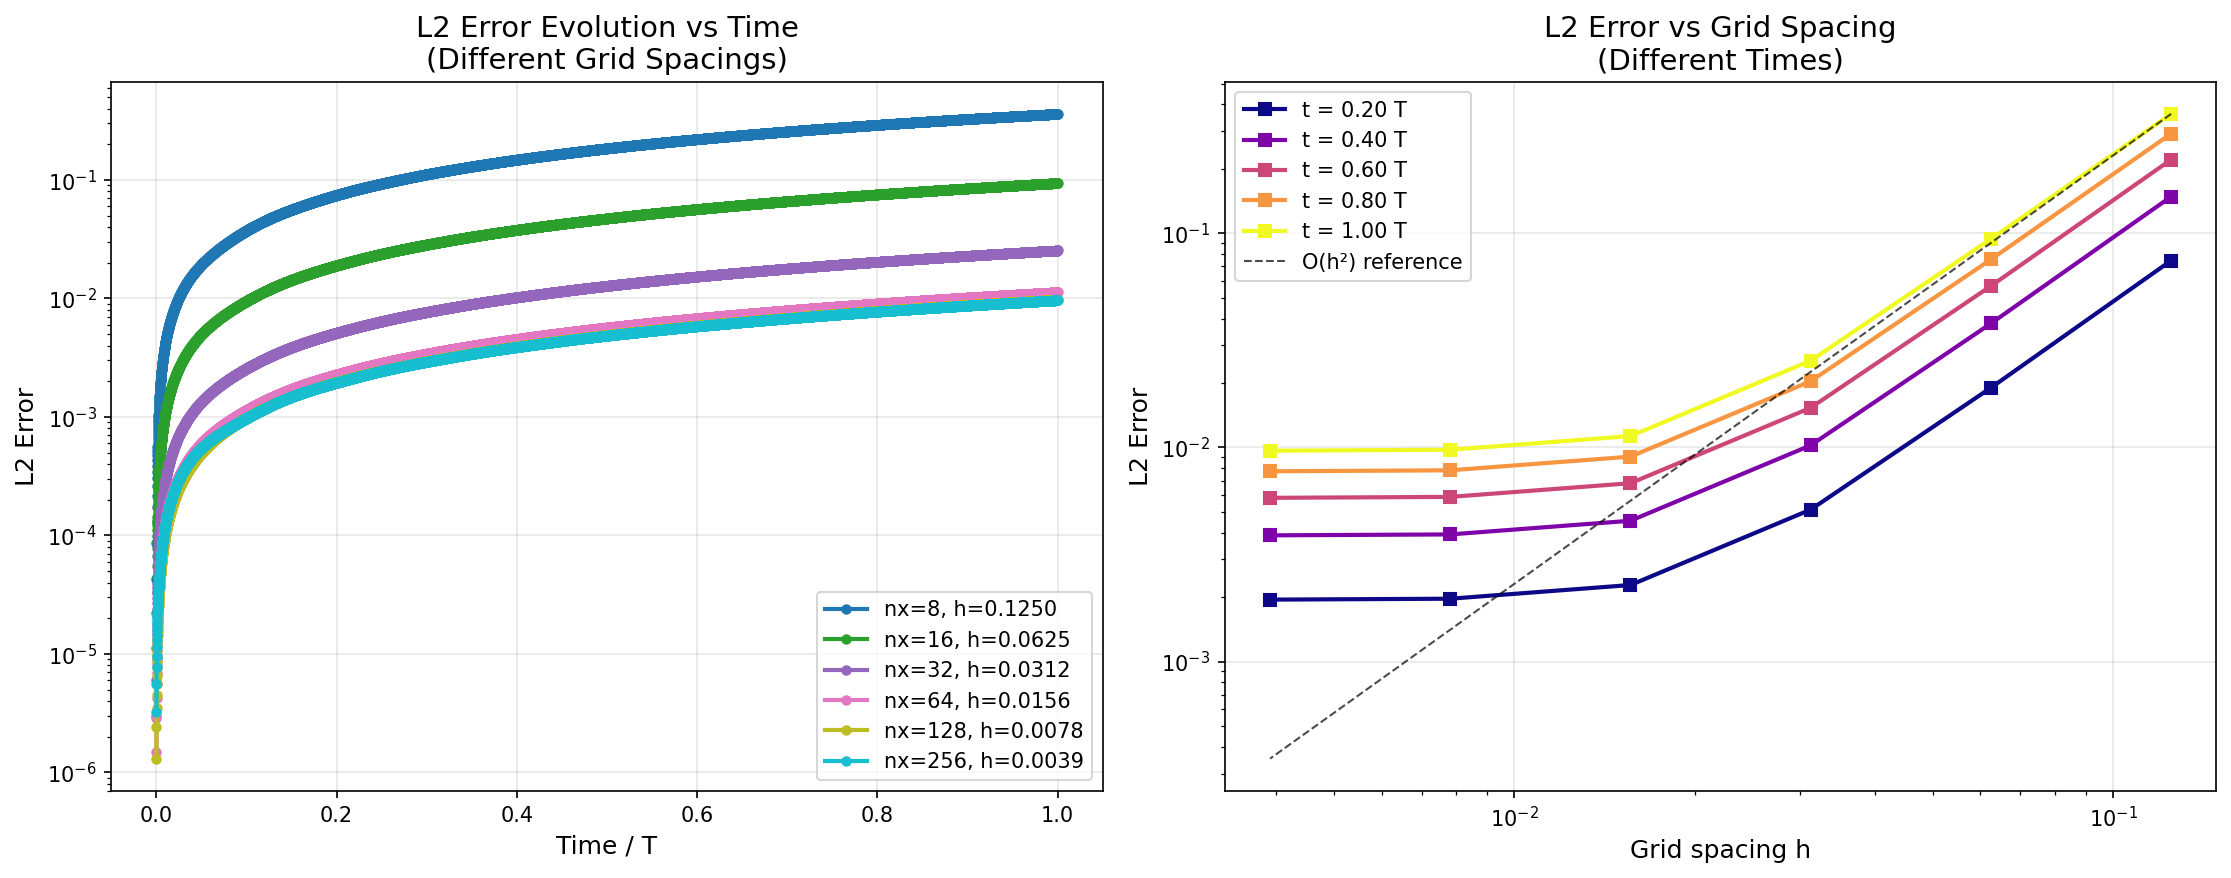
\includegraphics[width=0.8\textwidth, trim=0cm 0cm 18.1cm 0cm, clip]{figures/2d_error_analysis.png}
  \caption{2D Error Analysis}
  \label{fig:2d_error_analysis}
\end{figure}

\begin{figure}[h]
  \centering
  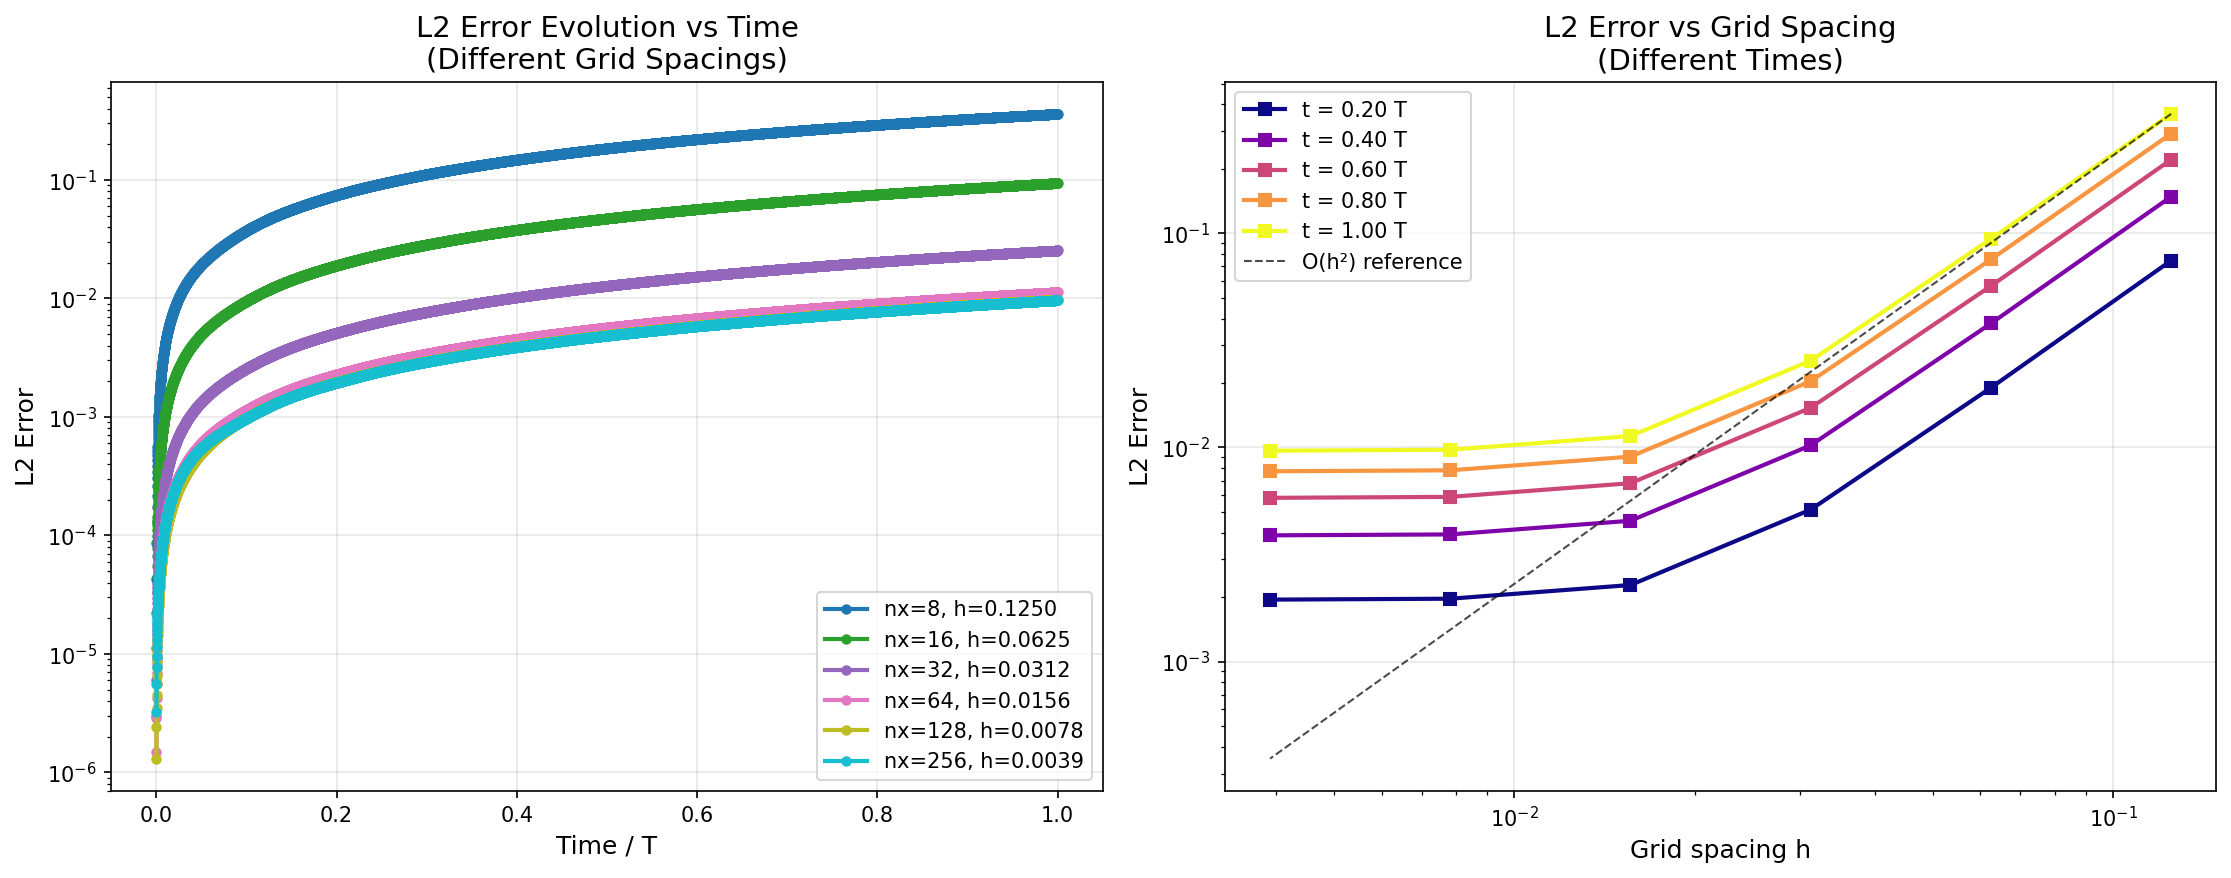
\includegraphics[width=0.8\textwidth, trim=19cm 0cm 0cm 0cm, clip]{figures/2d_error_analysis.png}
  \caption{2D Error Analysis}
  \label{fig:2d_error_analysis_2}
\end{figure}

\subsubsection*{PINN Solution}
We use the previously derived PINN loss functional to train a neural network to approximate the solution of the free Schrödinger equation, by setting the potential \( V(x,t) = 0 \) and the initial condition \( u_0(x,y) = \sin(\pi x)\sin(\pi y) \).
Through a hyperparameter optimization we found the following parameters to work well:
\begin{itemize}
  \item Hidden layers: 3
  \item Neurons per layer: 128
  \item Activation function: Tanh
  \item Learning rate: 0.00003
  \item Interior collocation points: 50000
  \item Boundary and initial collocation points: 25000 each
  \item $\lambda_{\mathrm{PDE}} = 1.0$, $\lambda_{\mathrm{IC}} = 1.0$, $\lambda_{\mathrm{BC}} = 1.0$, $\lambda_{\mathrm{norm}} = 0$
\end{itemize}
The evolution of the solution computed by the PINN is shown in Figure \ref{fig:free_solution_evolution_pinn}.
We can see that the PINN is able to approximate the initial and boundary condition, but does not show the behavior of the analytical solution.
Instead the solution converges to the trivial solution \( u(x,y,t) = 0 \) over time, which also satisfies the PDE and the boundary conditions.
This behaviour could not be resolved by adding the normalization term to the loss functional, which was intended to prevent the trivial solution.
\begin{figure}[h]
  \centering
  \begin{subfigure}[b]{0.3\textwidth}
    \centering
    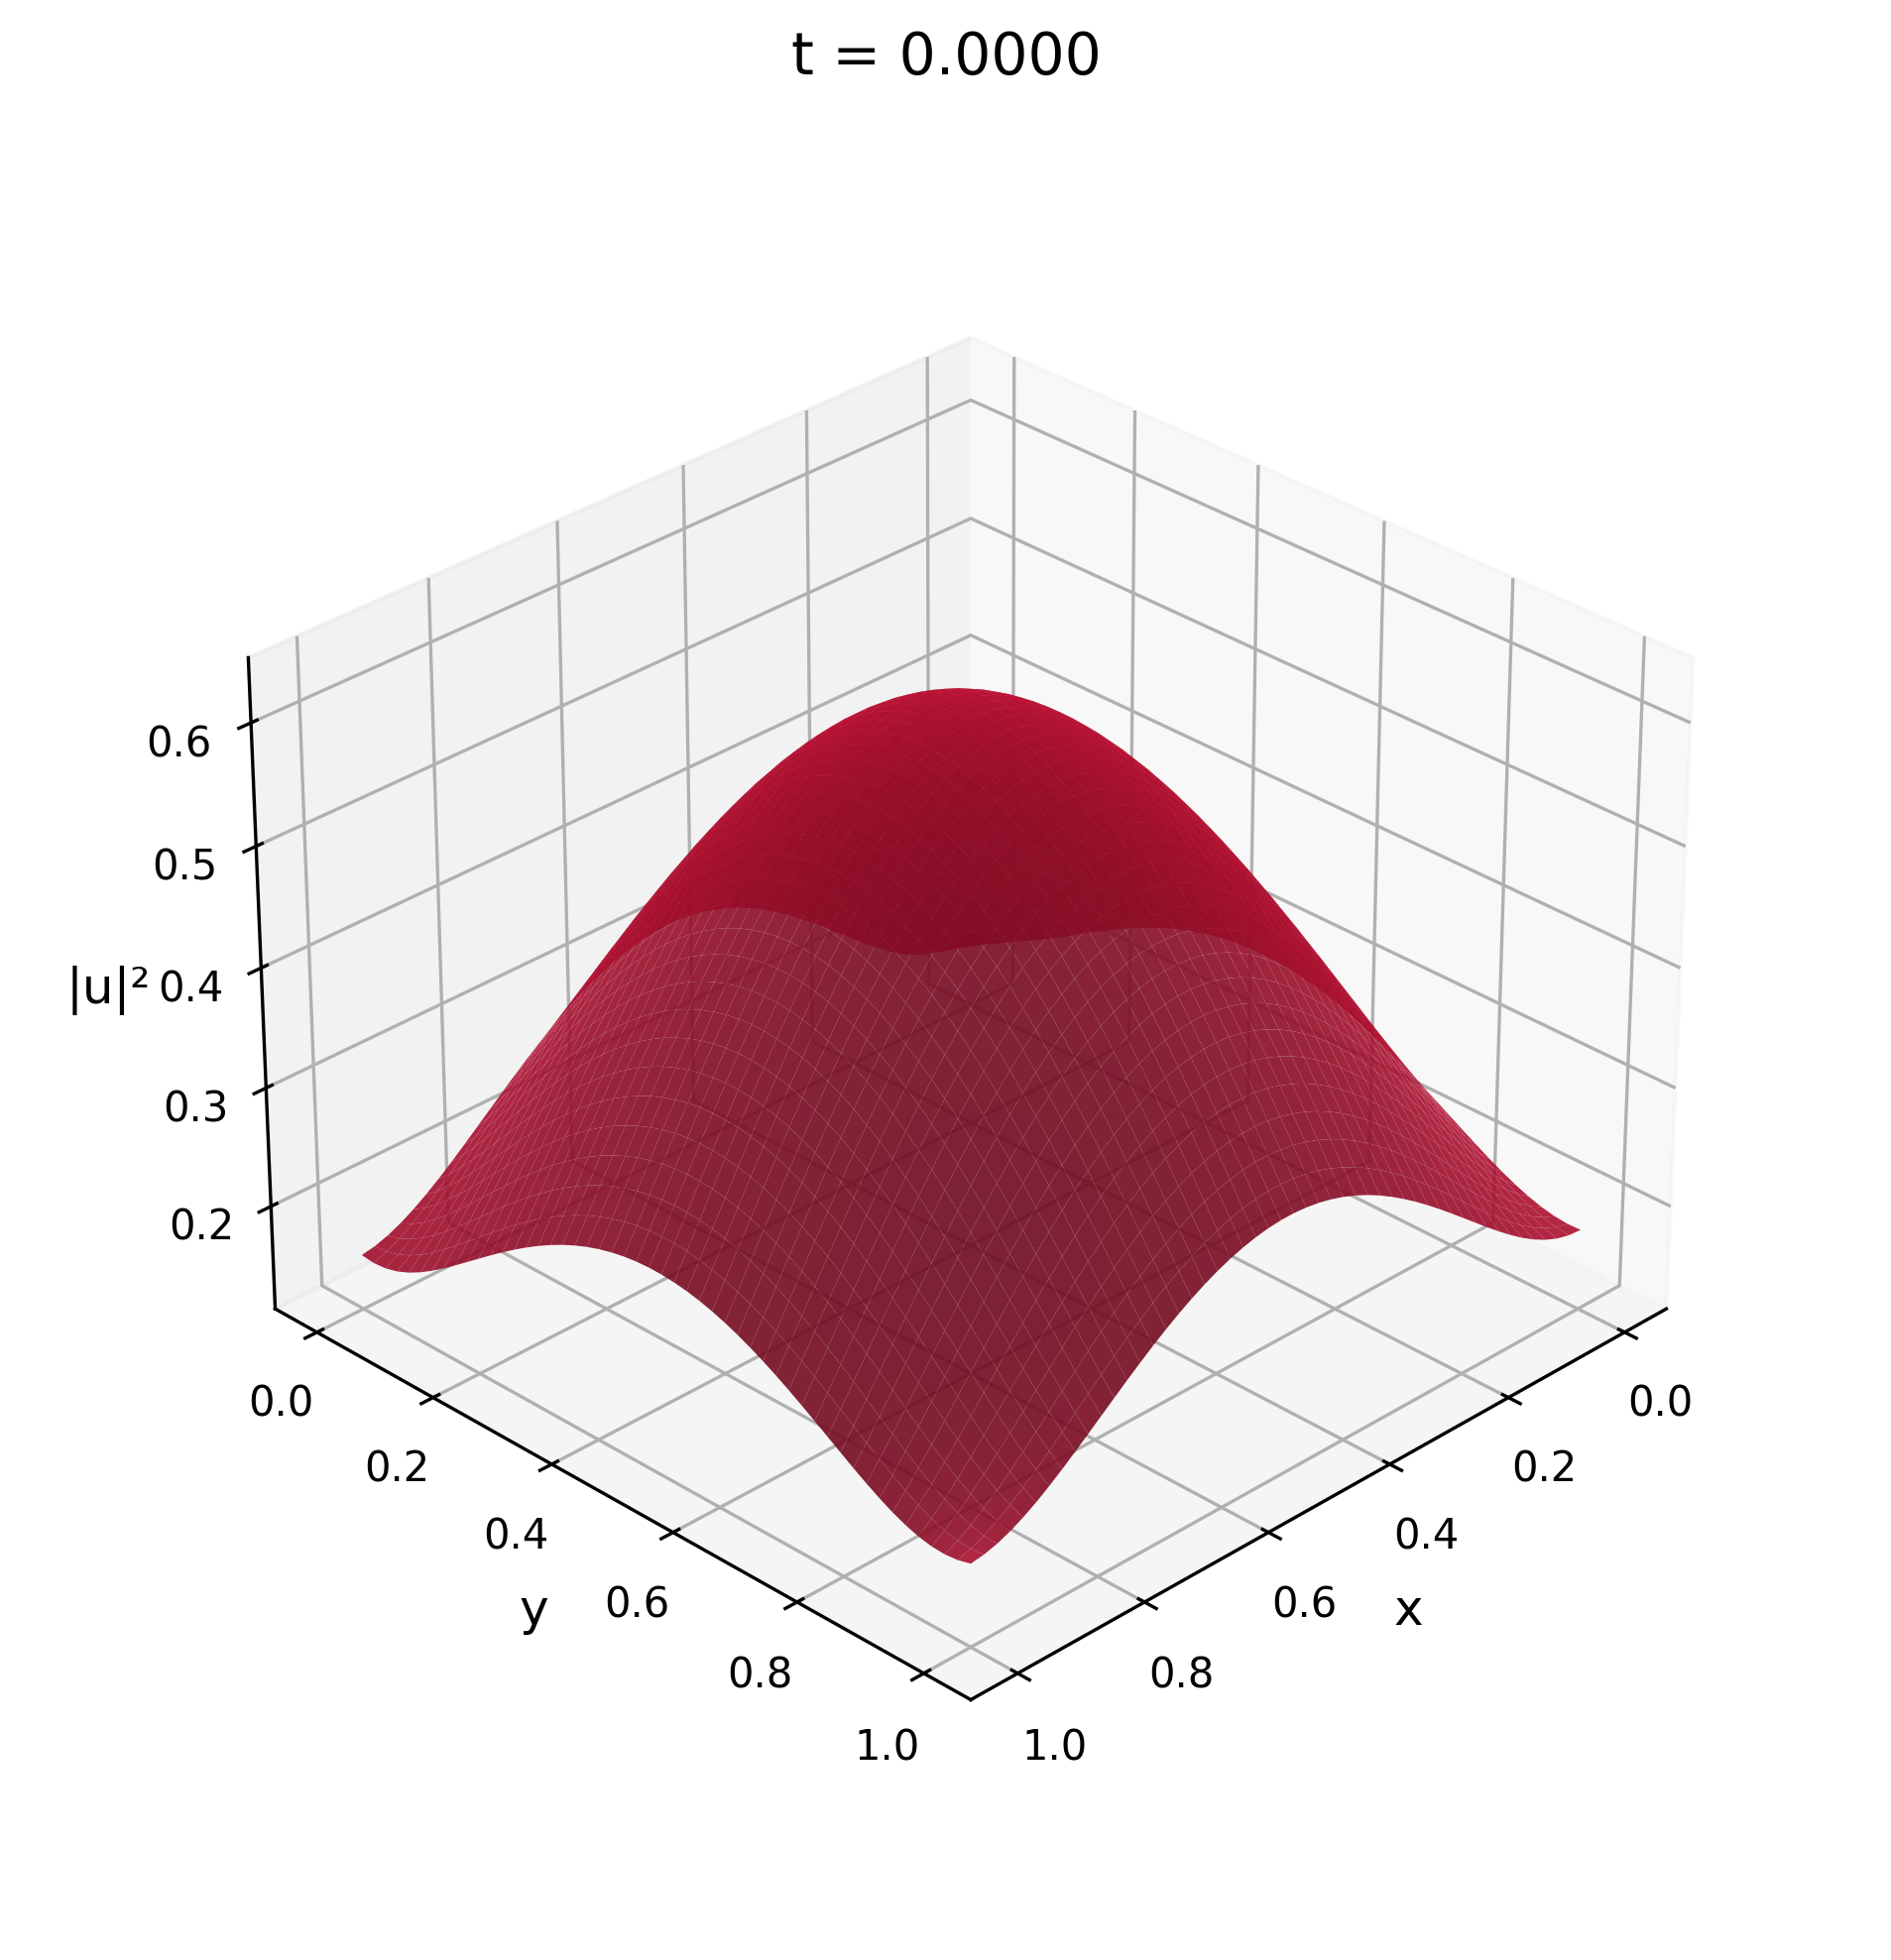
\includegraphics[width=\textwidth, trim=0cm 0cm 0cm 1cm, clip]{figures/pinn_frame_0000.png}
    \caption{t = 0.0}
  \end{subfigure}
  \hfill
  \begin{subfigure}[b]{0.3\textwidth}
    \centering
    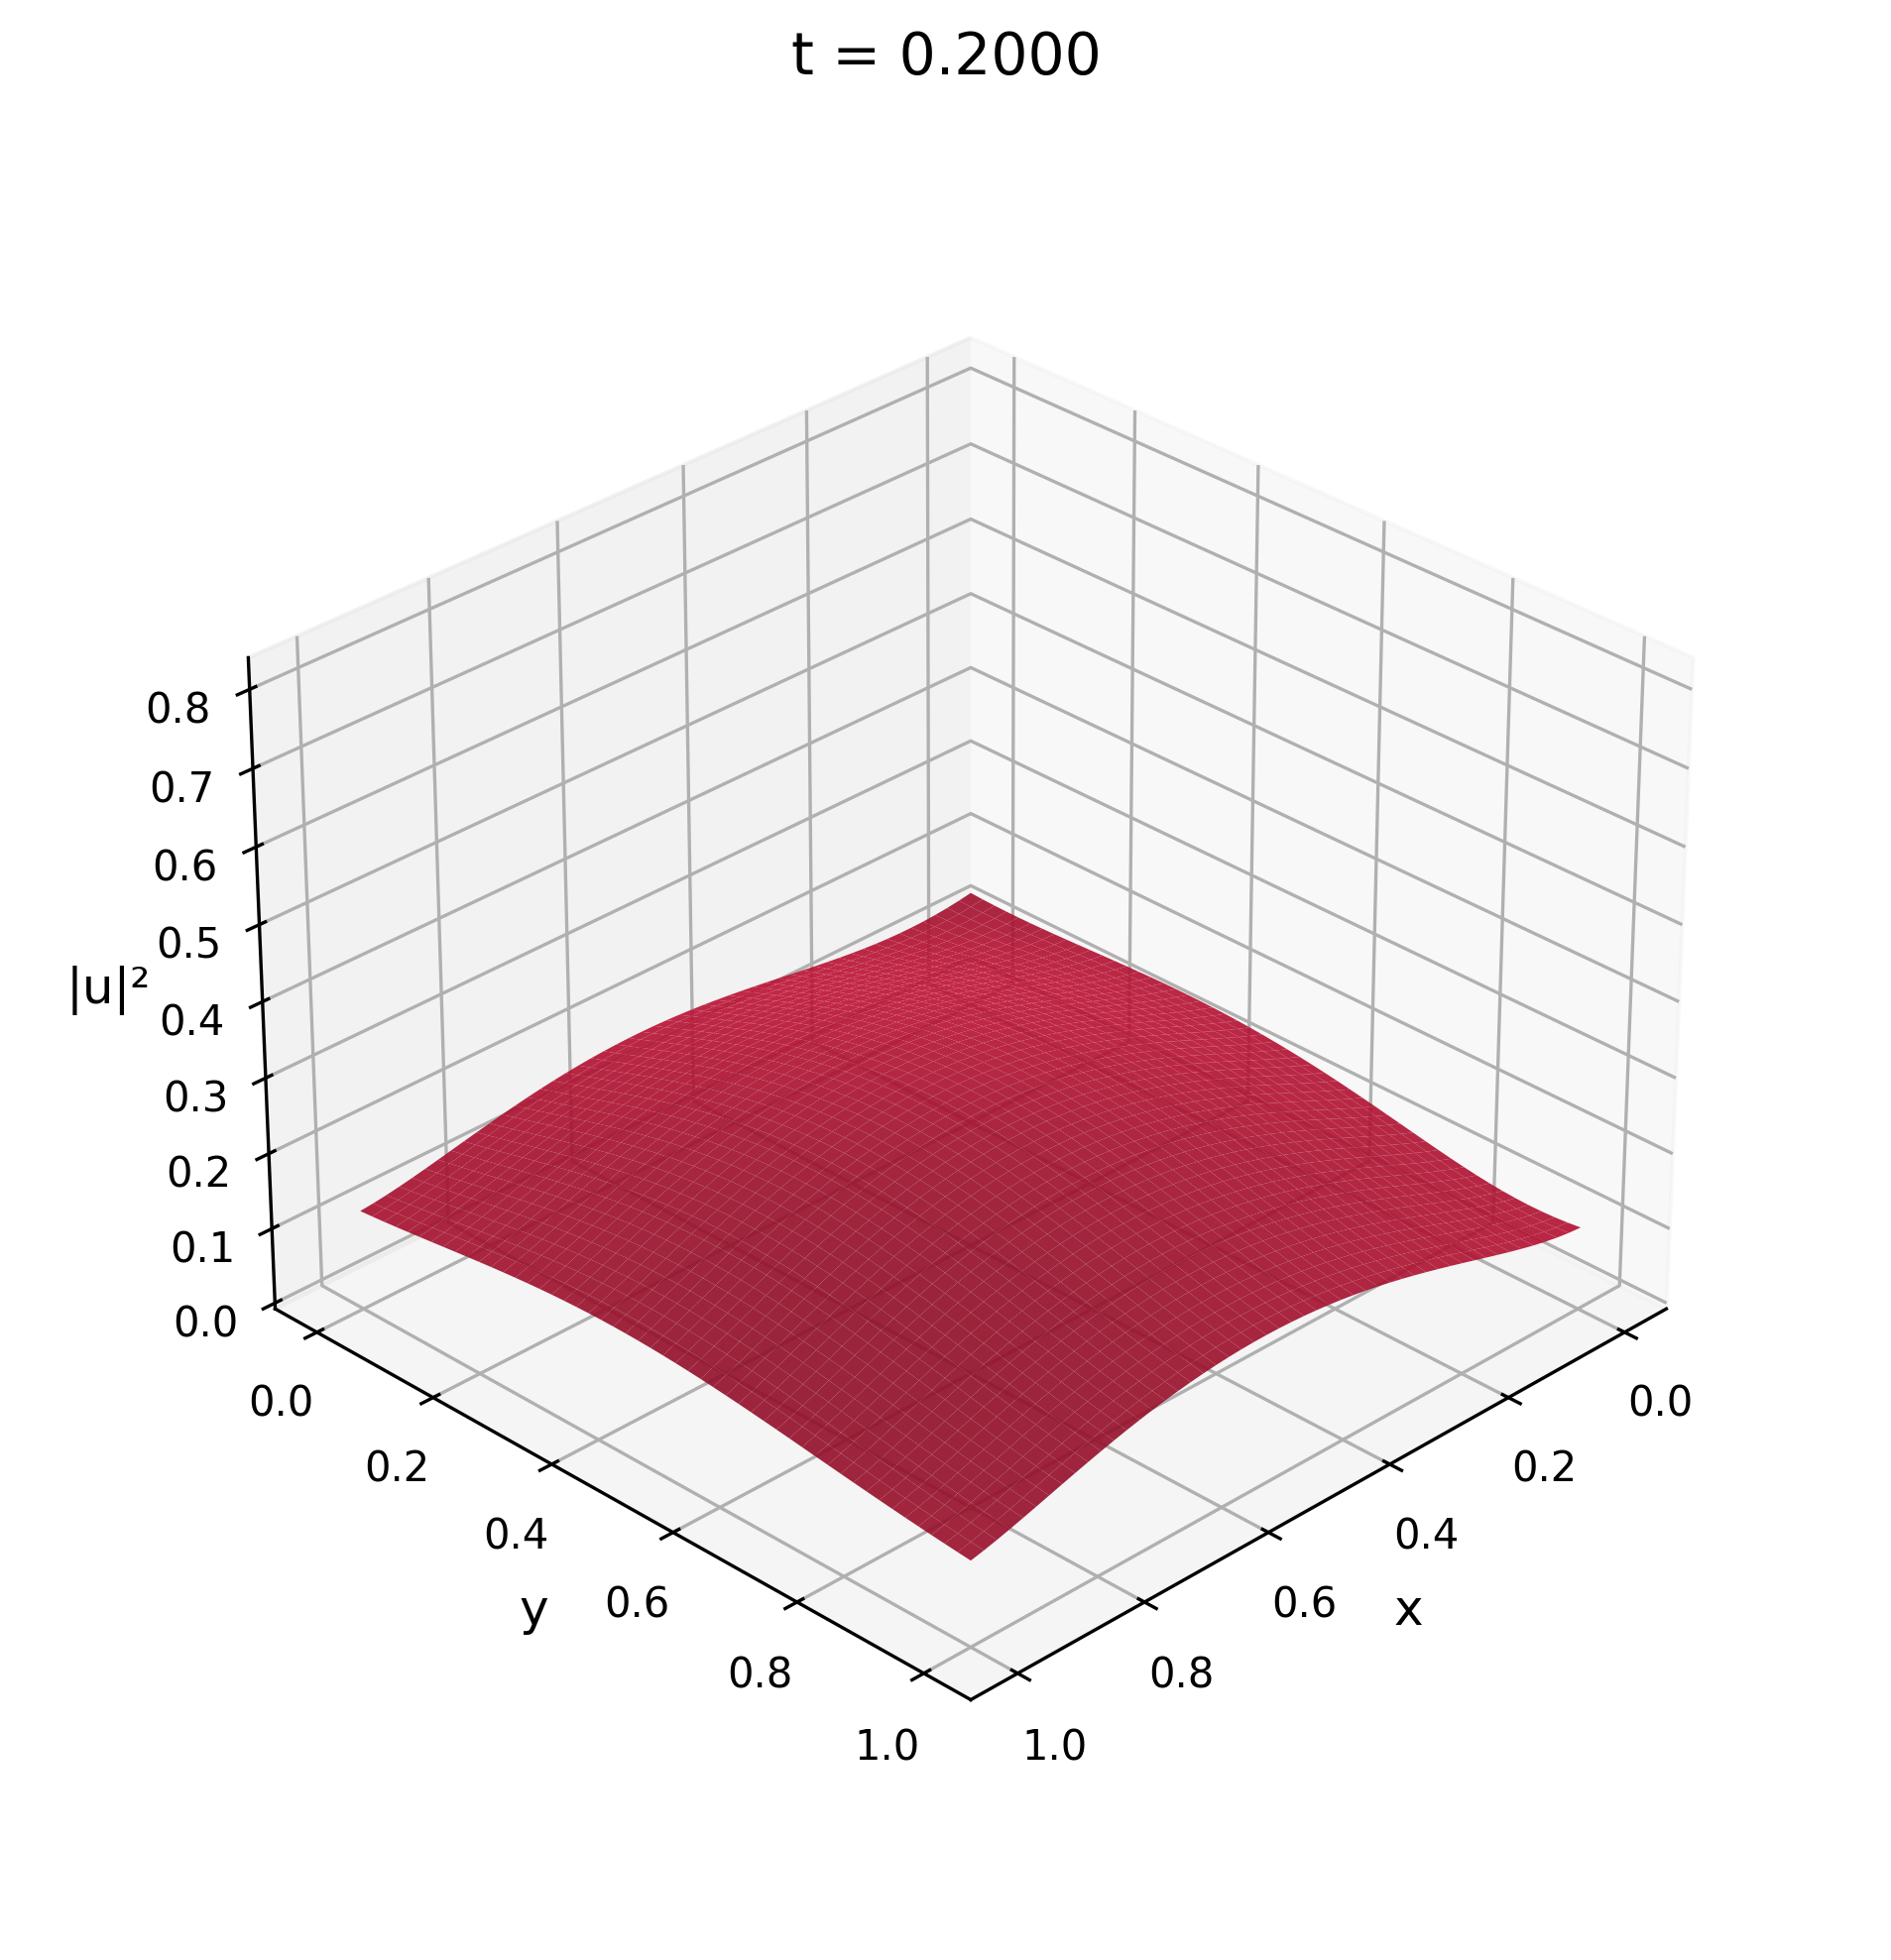
\includegraphics[width=\textwidth, trim=0cm 0cm 0cm 1cm, clip]{figures/pinn_frame_0010.png}
    \caption{t = 0.2}
  \end{subfigure}
  \hfill
  \begin{subfigure}[b]{0.3\textwidth}
    \centering
    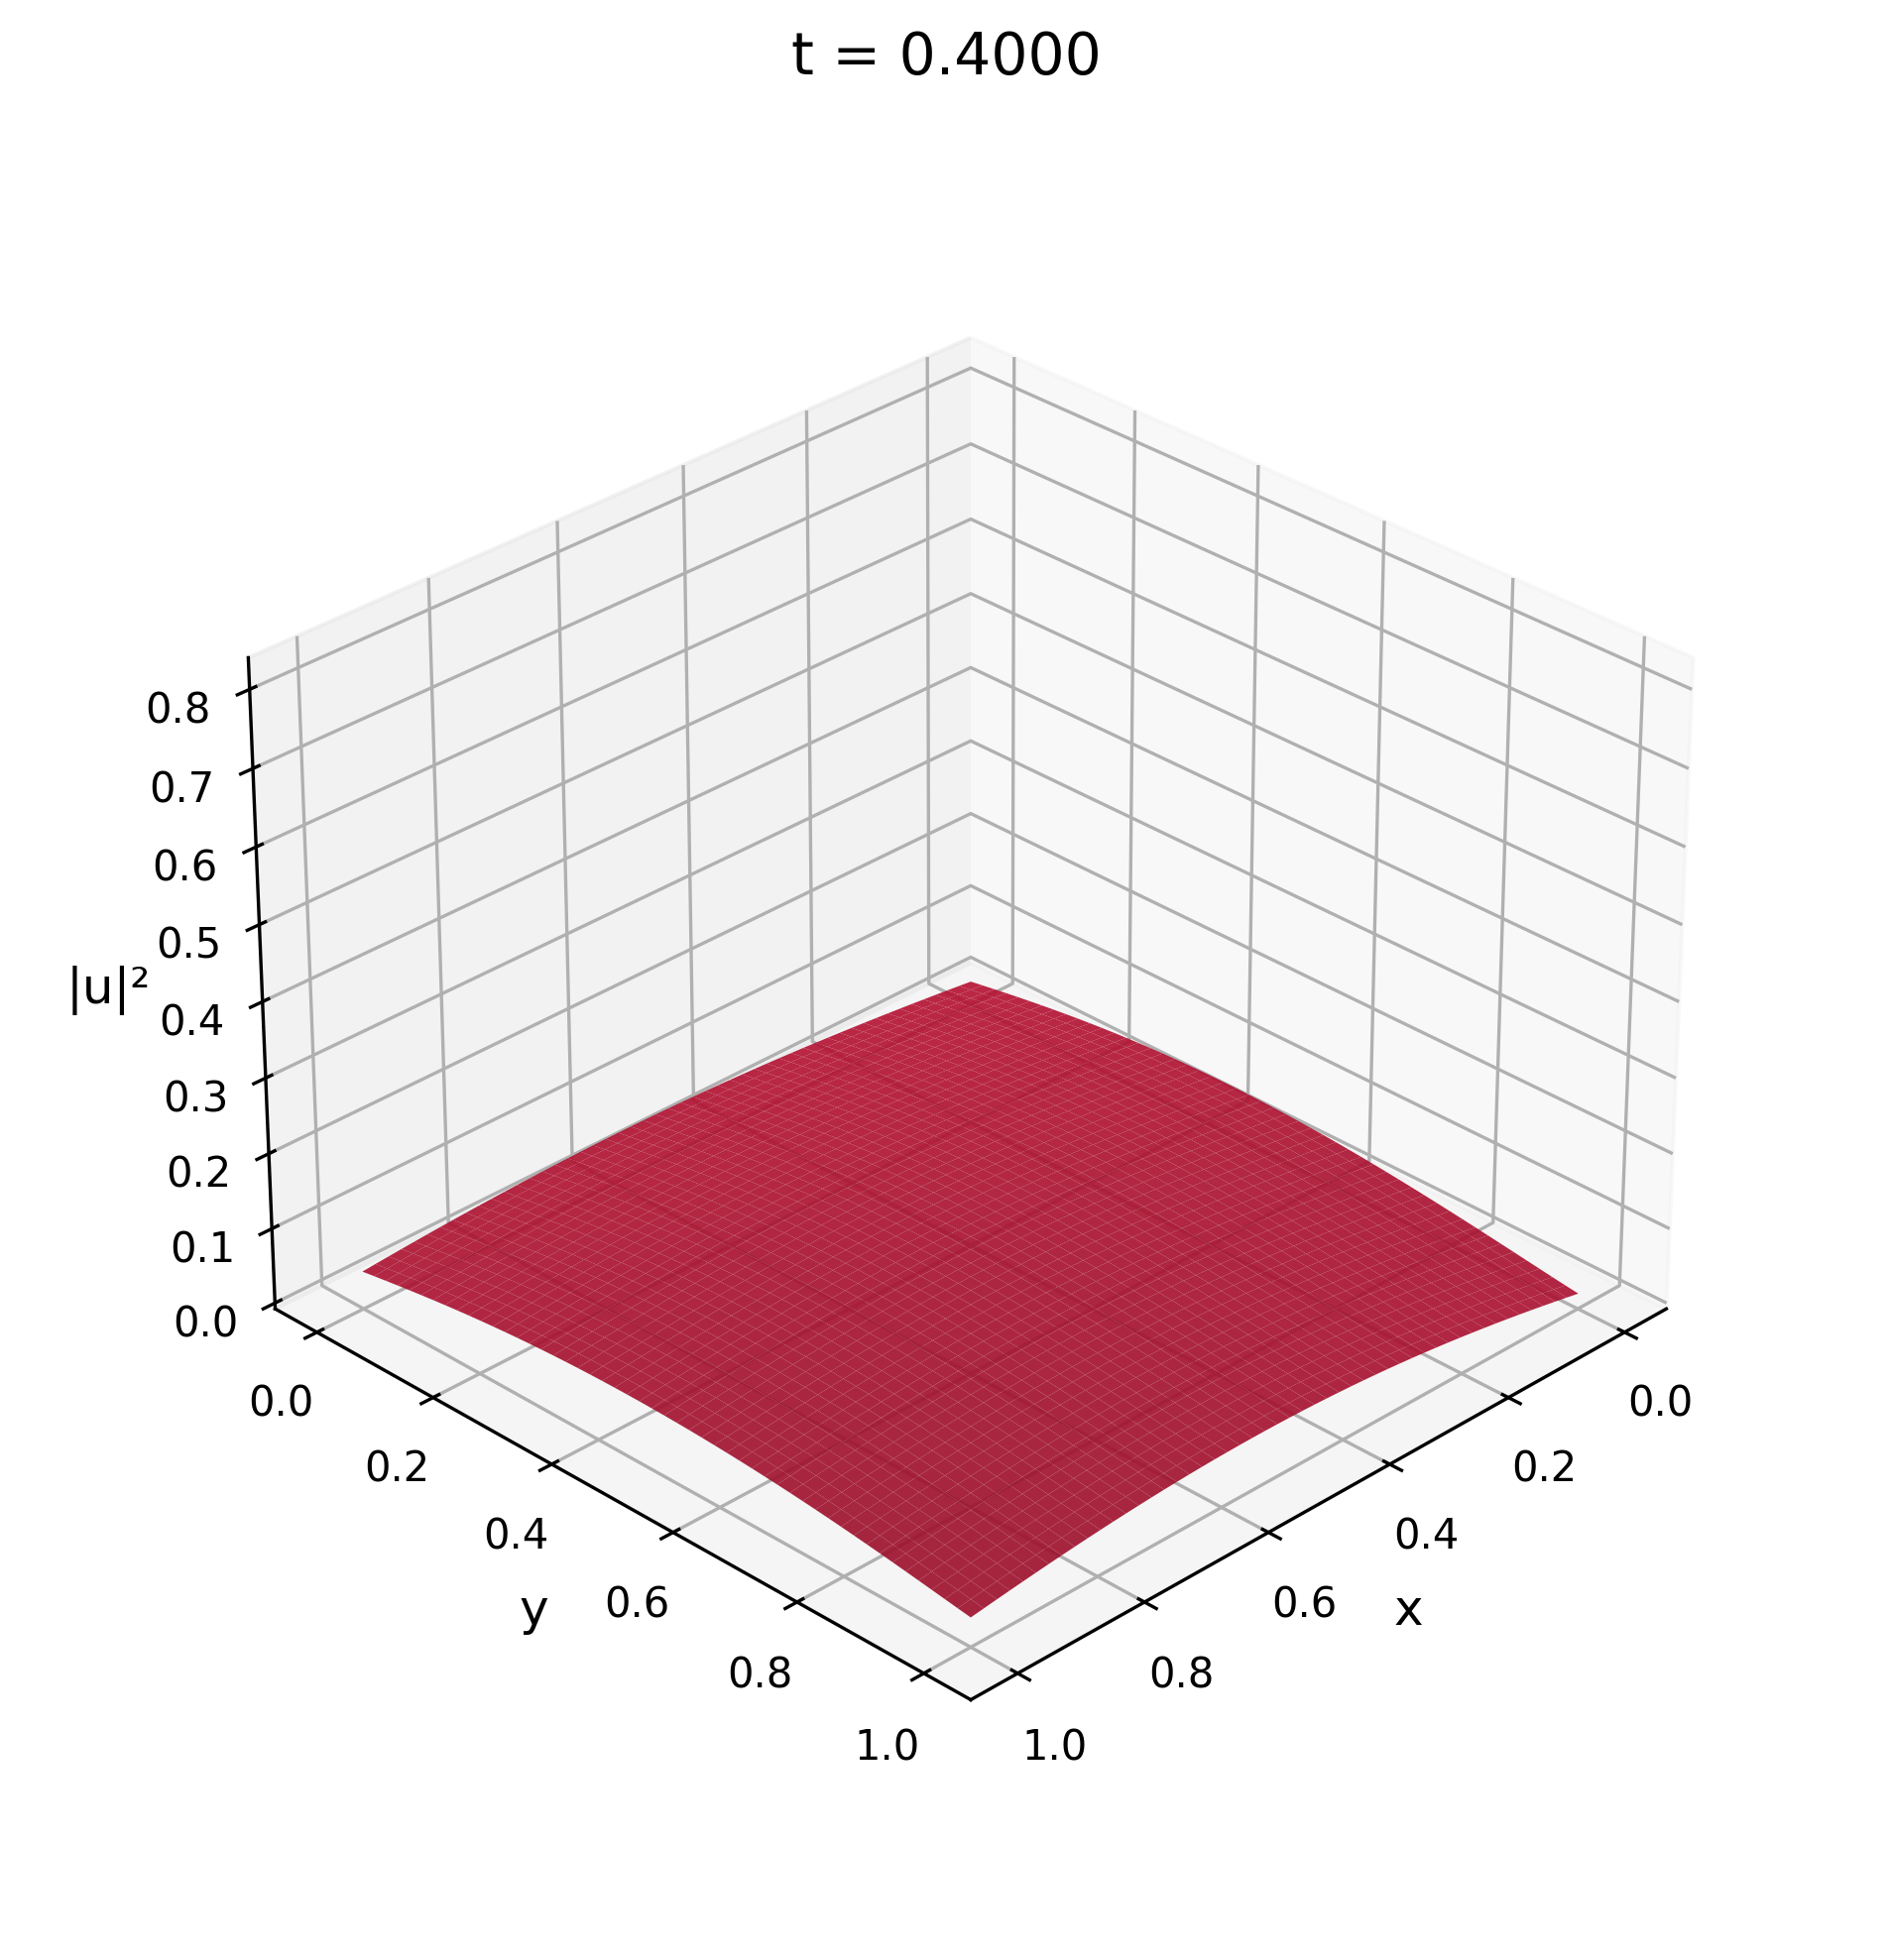
\includegraphics[width=\textwidth, trim=0cm 0cm 0cm 1cm, clip]{figures/pinn_frame_0020.png}
    \caption{t = 0.4}
  \end{subfigure}
  
  \vspace{0.5cm}
  
  \begin{subfigure}[b]{0.3\textwidth}
    \centering
    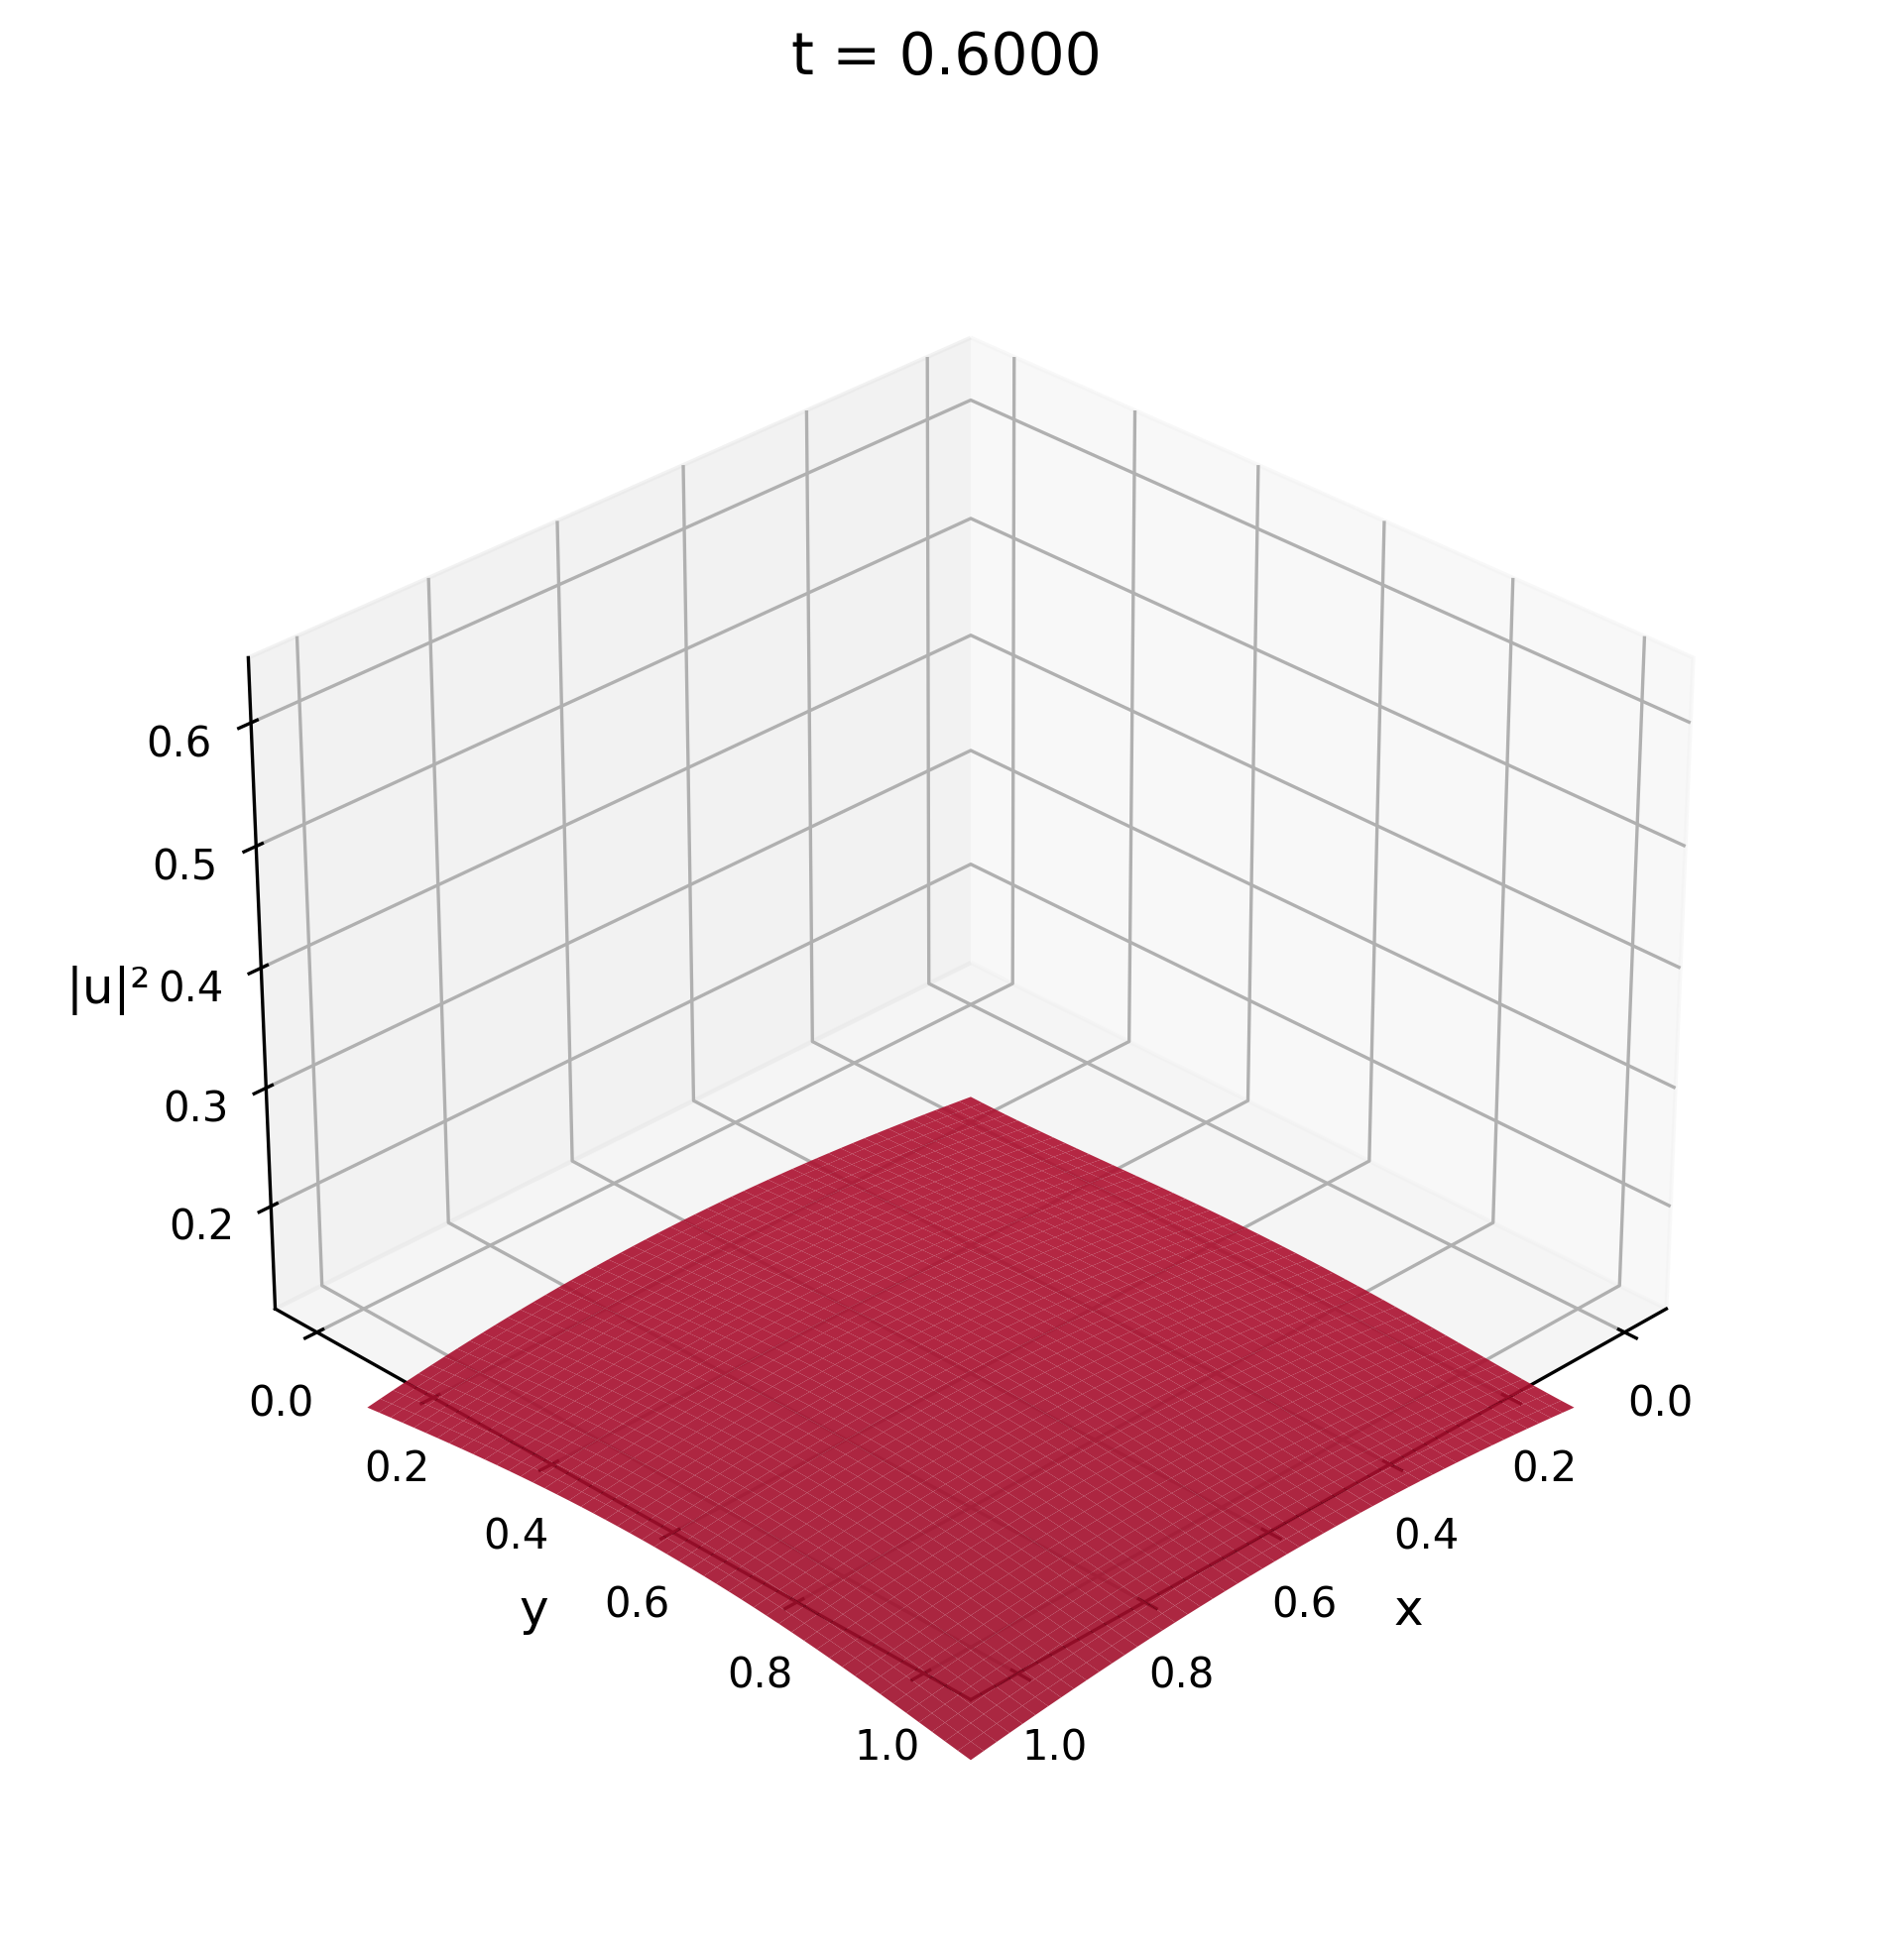
\includegraphics[width=\textwidth, trim=0cm 0cm 0cm 1cm, clip]{figures/pinn_frame_0030.png}
    \caption{t = 0.6}
  \end{subfigure}
  \hfill
  \begin{subfigure}[b]{0.3\textwidth}
    \centering
    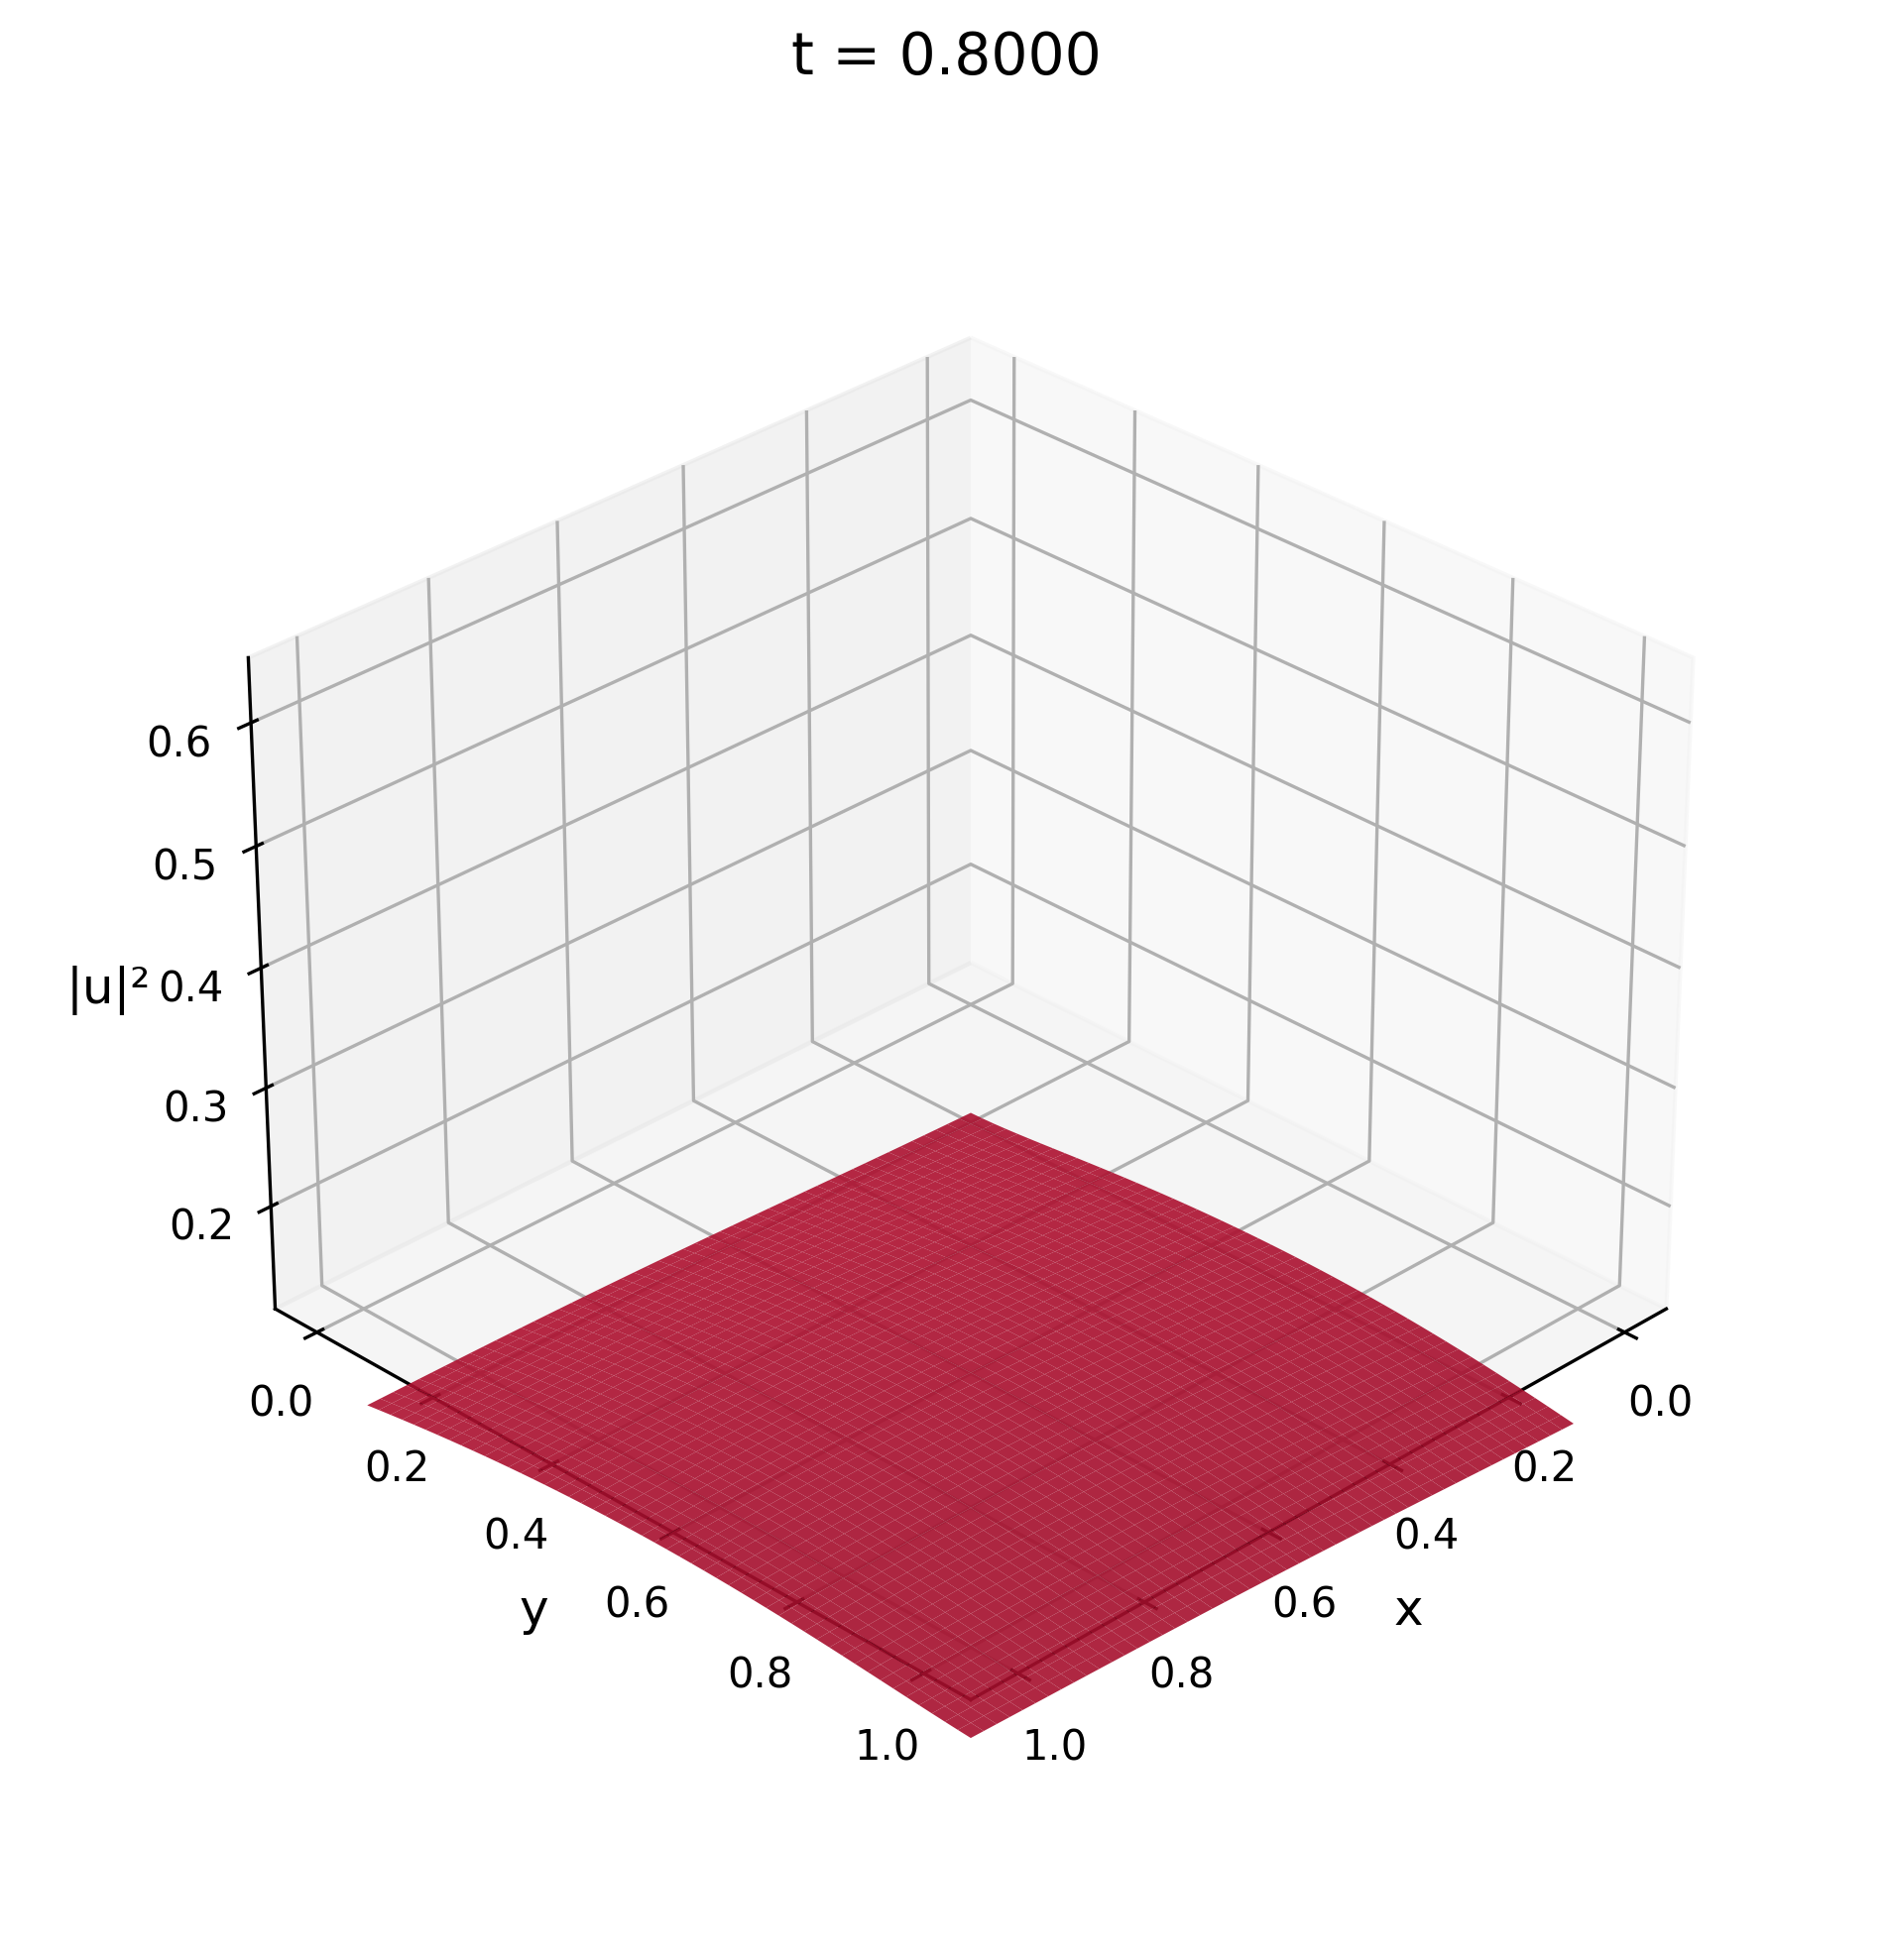
\includegraphics[width=\textwidth, trim=0cm 0cm 0cm 1cm, clip]{figures/pinn_frame_0040.png}
    \caption{t = 0.8}
  \end{subfigure}
  \hfill
  \begin{subfigure}[b]{0.3\textwidth}
    \centering
    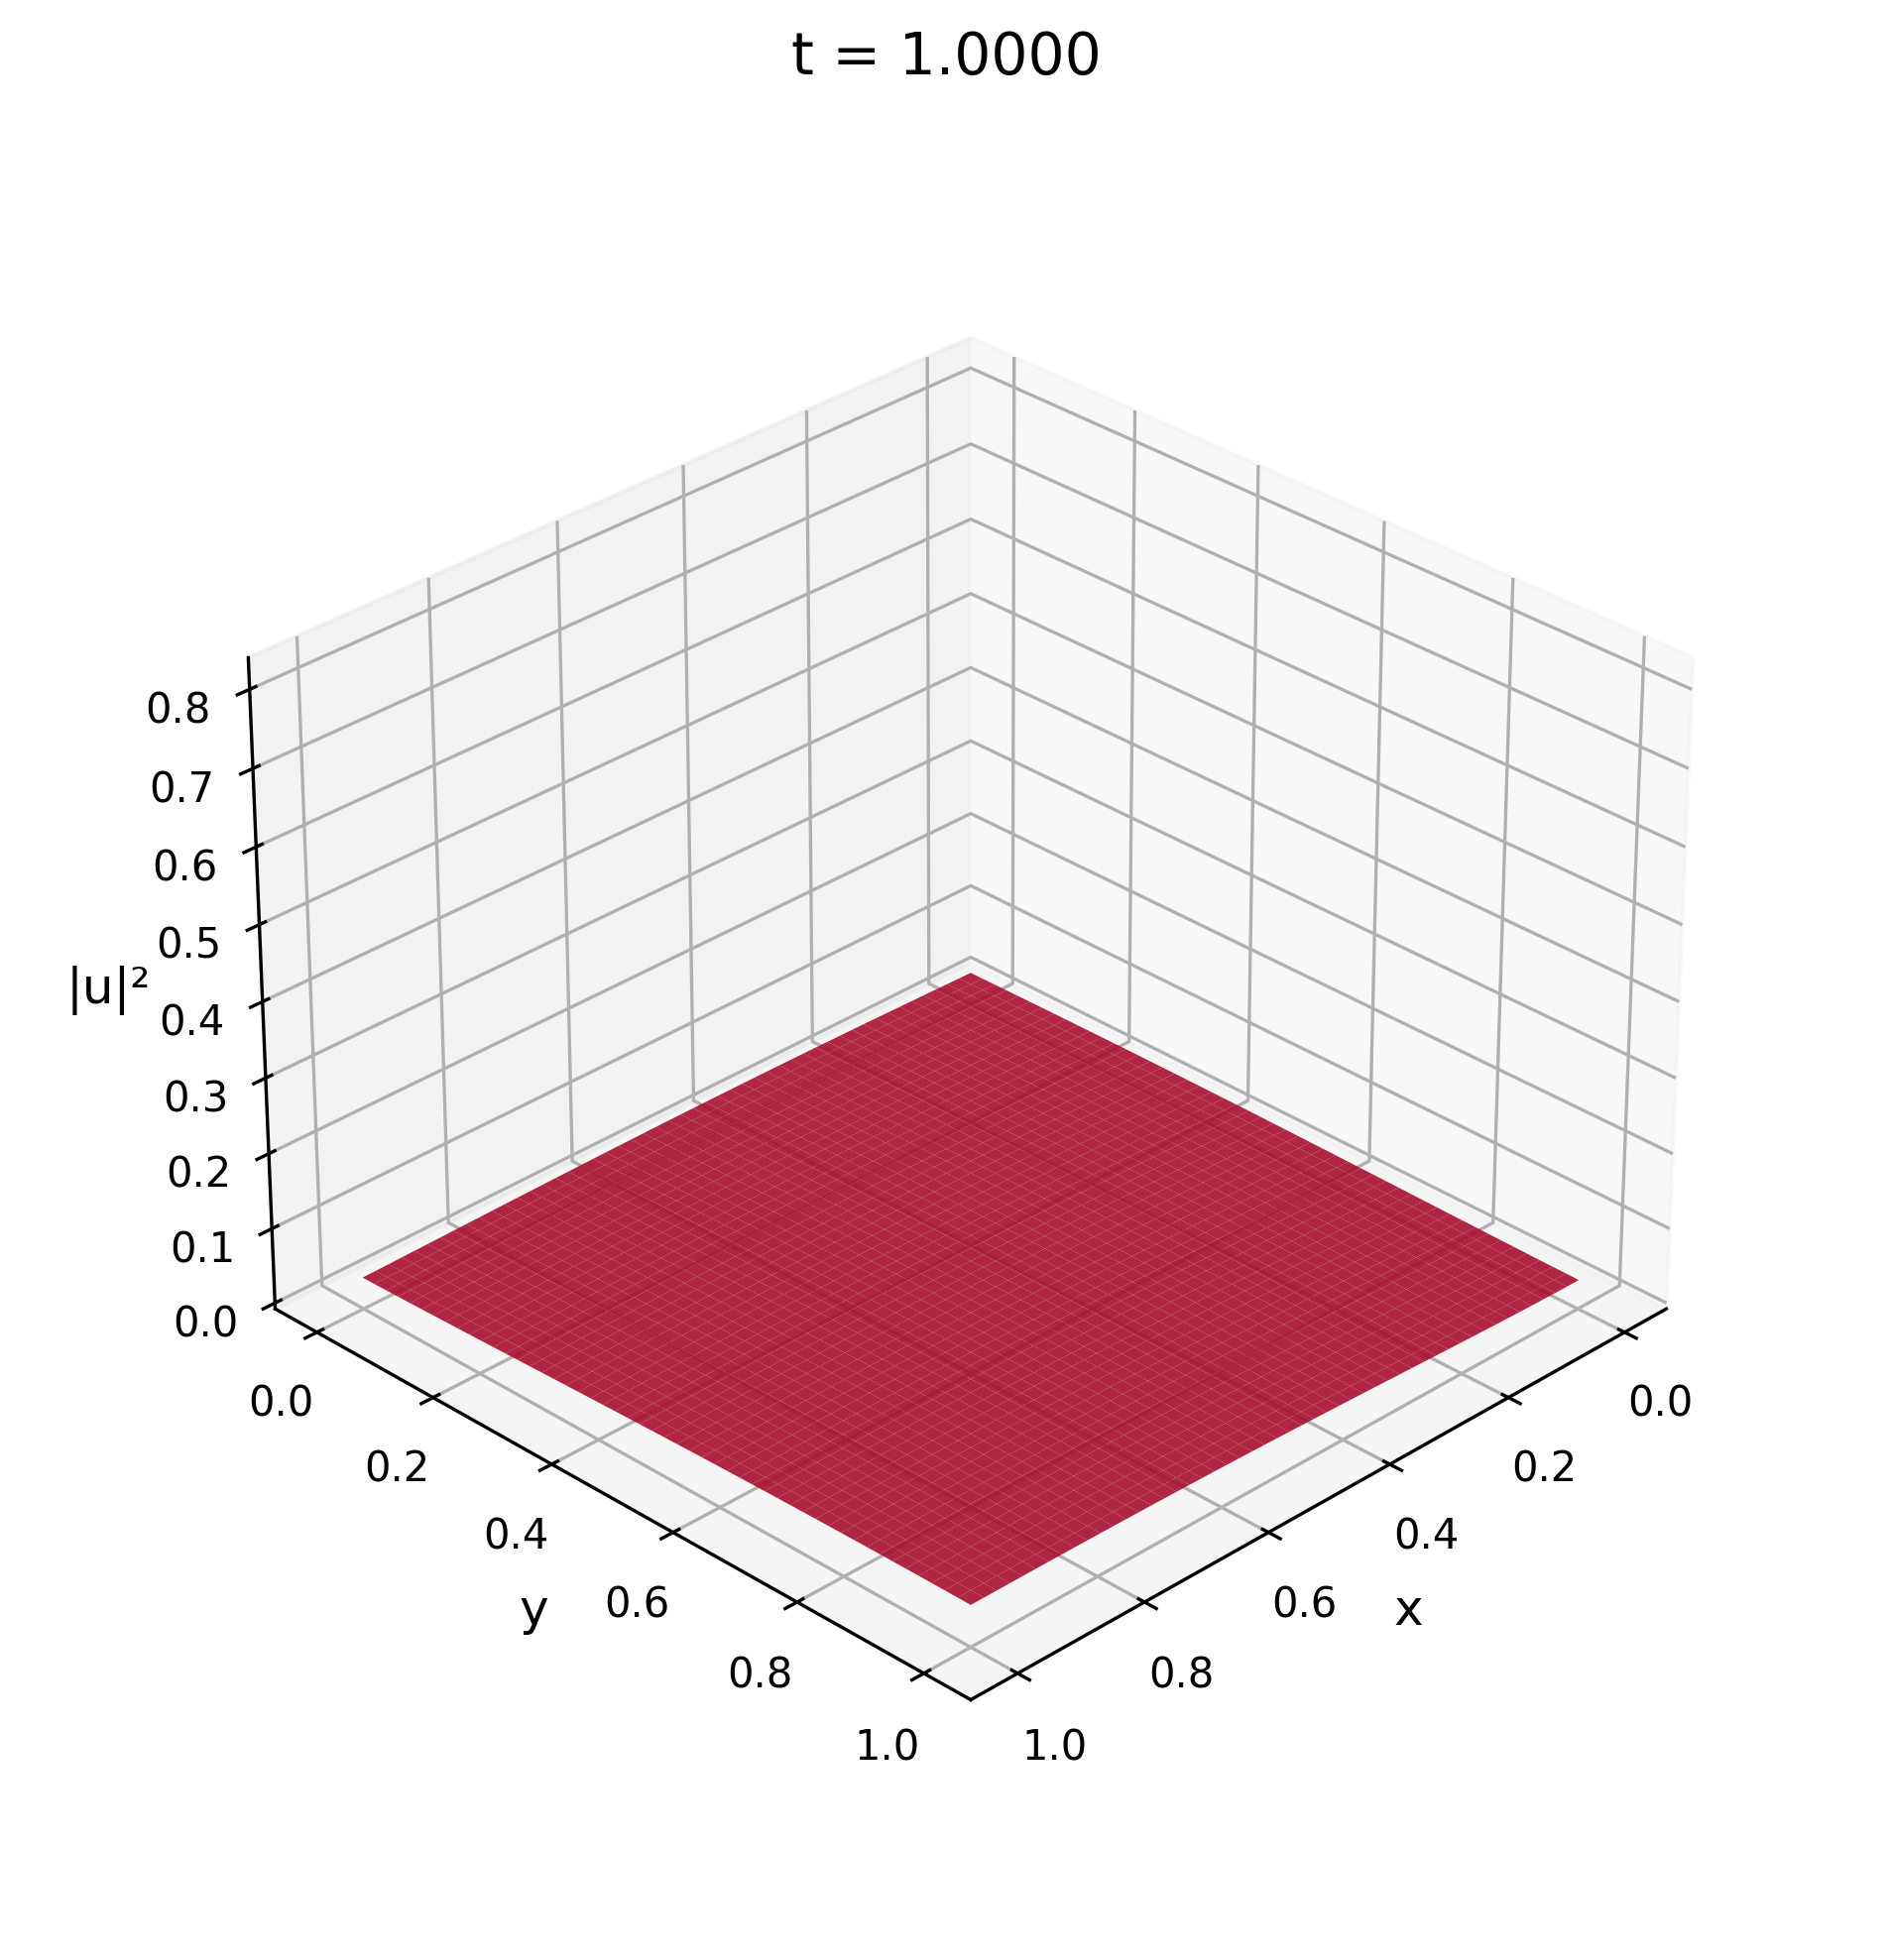
\includegraphics[width=\textwidth, trim=0cm 0cm 0cm 1cm, clip]{figures/pinn_frame_0050.png}
    \caption{t = 1.0}
  \end{subfigure}
  \caption{Time evolution of the solution of the free Schrödinger equation, obtained with the PINN.}
  \label{fig:free_solution_evolution_pinn}
\end{figure}

\subsubsection*{Comparison of FEM and PINN}
Finite Element Methods have the advantage of a well-established theory with which the convergence and stability of the solution can be guaranteed.
As well as the desired accuracy can be achieved by refining the mesh and the time step size.
Contrary to PINNs, where many different hyperparameters have an influence on the solution and therefore the accuracy. 
Additionally in this case the PINN is not capable of approximating the analytical solution, which is a major drawback.
We aim to resolve this problem to have the ability to compare the solutions of both methods.

\subsection*{Problem 2: Schrödinger Equation with Time-Dependent Model Potential}

\subsubsection*{The Model Potential}

\begin{figure}[h]
  \centering
  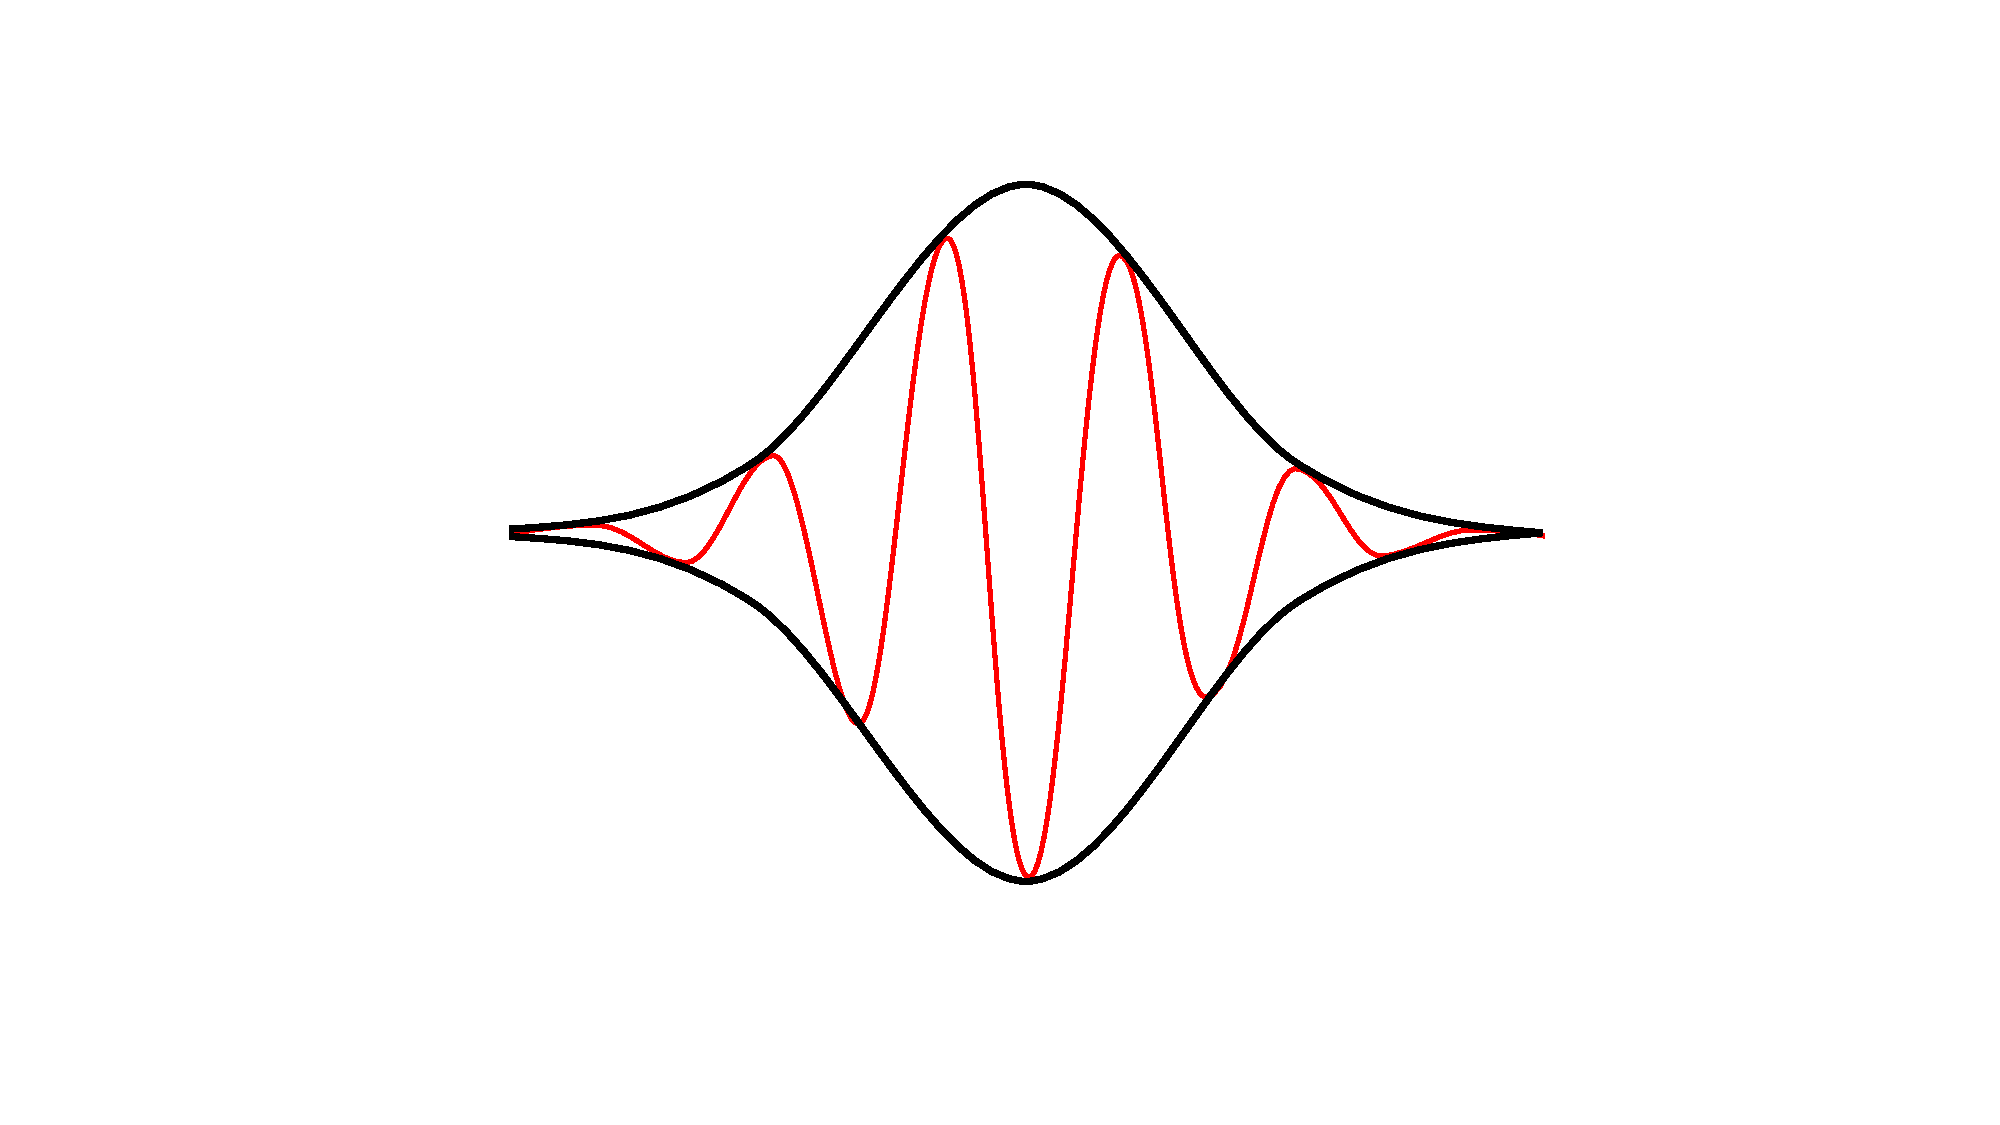
\includegraphics[width=0.7\textwidth,trim=2cm 2cm 2cm 2cm,clip]{figures/Figure3.pdf}
  \caption{Laser Pulse}
  \label{fig:laser_pulse}
\end{figure}



\begin{figure}[h]
  \centering
  \begin{subfigure}[b]{0.3\textwidth}
    \centering
    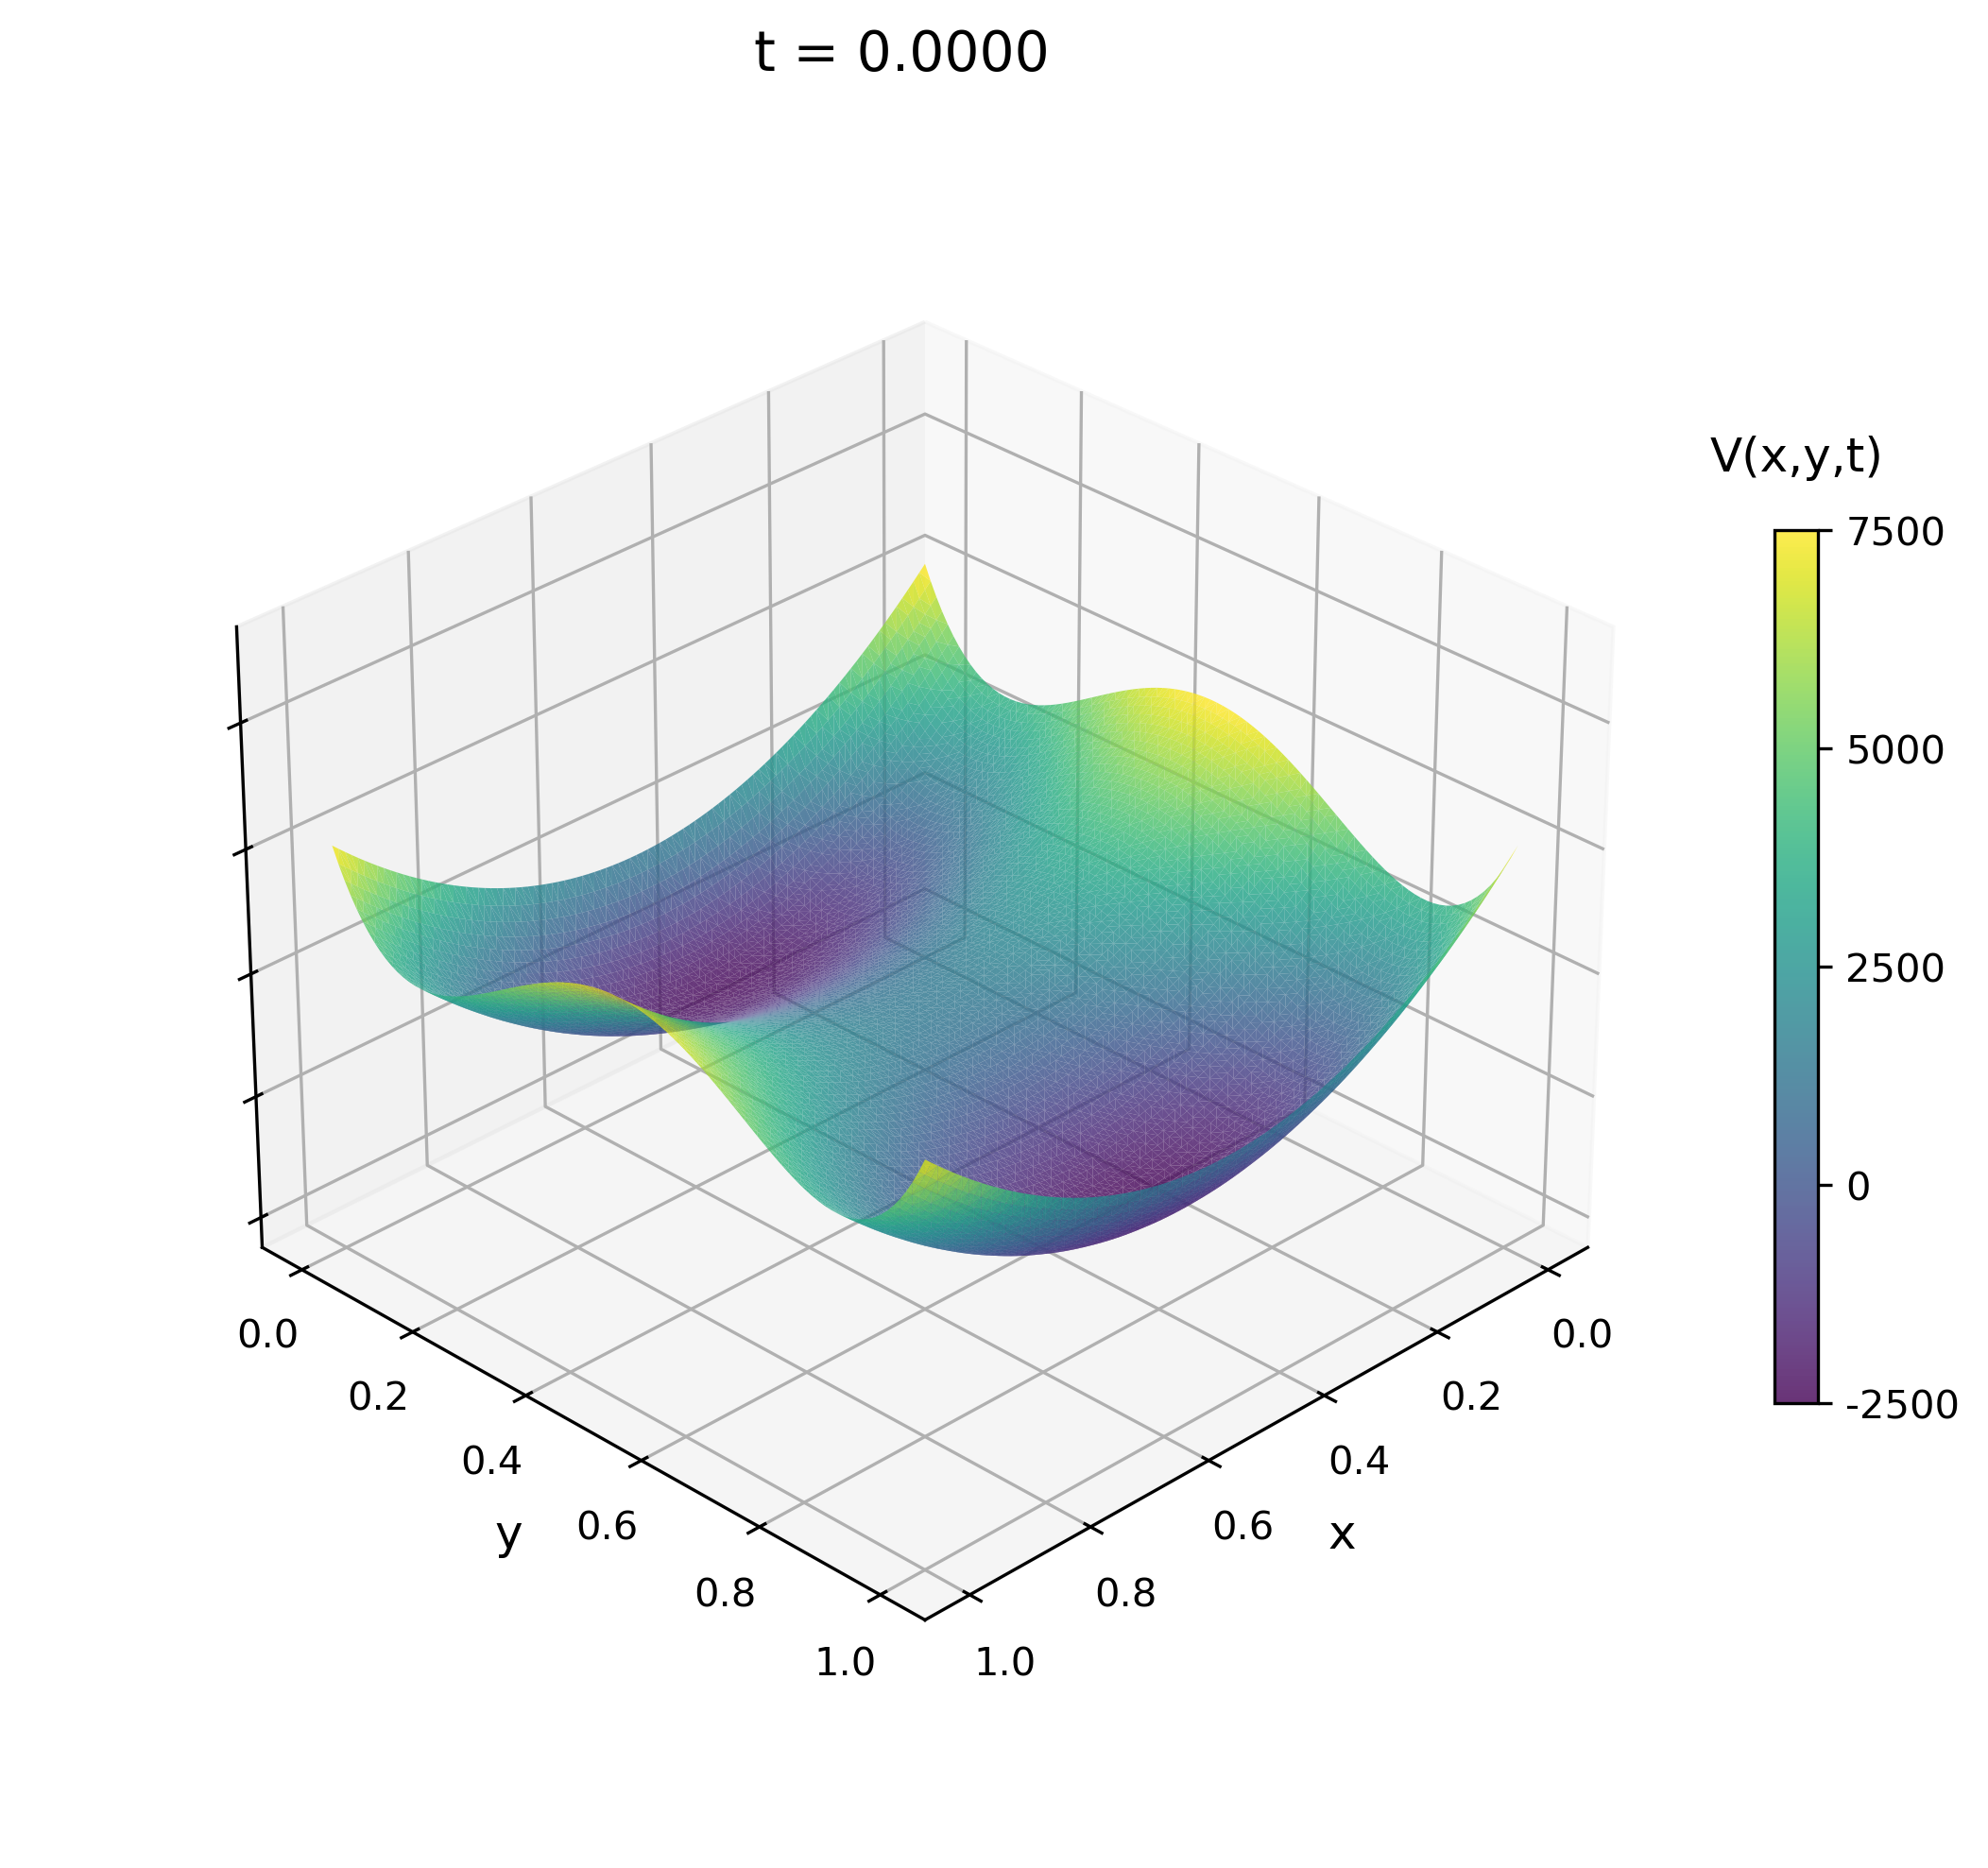
\includegraphics[width=\textwidth, trim=0cm 0cm 0cm 1cm, clip]{figures/potential_frame_0000.png}
    \caption{t = 0.0}
  \end{subfigure}
  \hfill
  \begin{subfigure}[b]{0.3\textwidth}
    \centering
    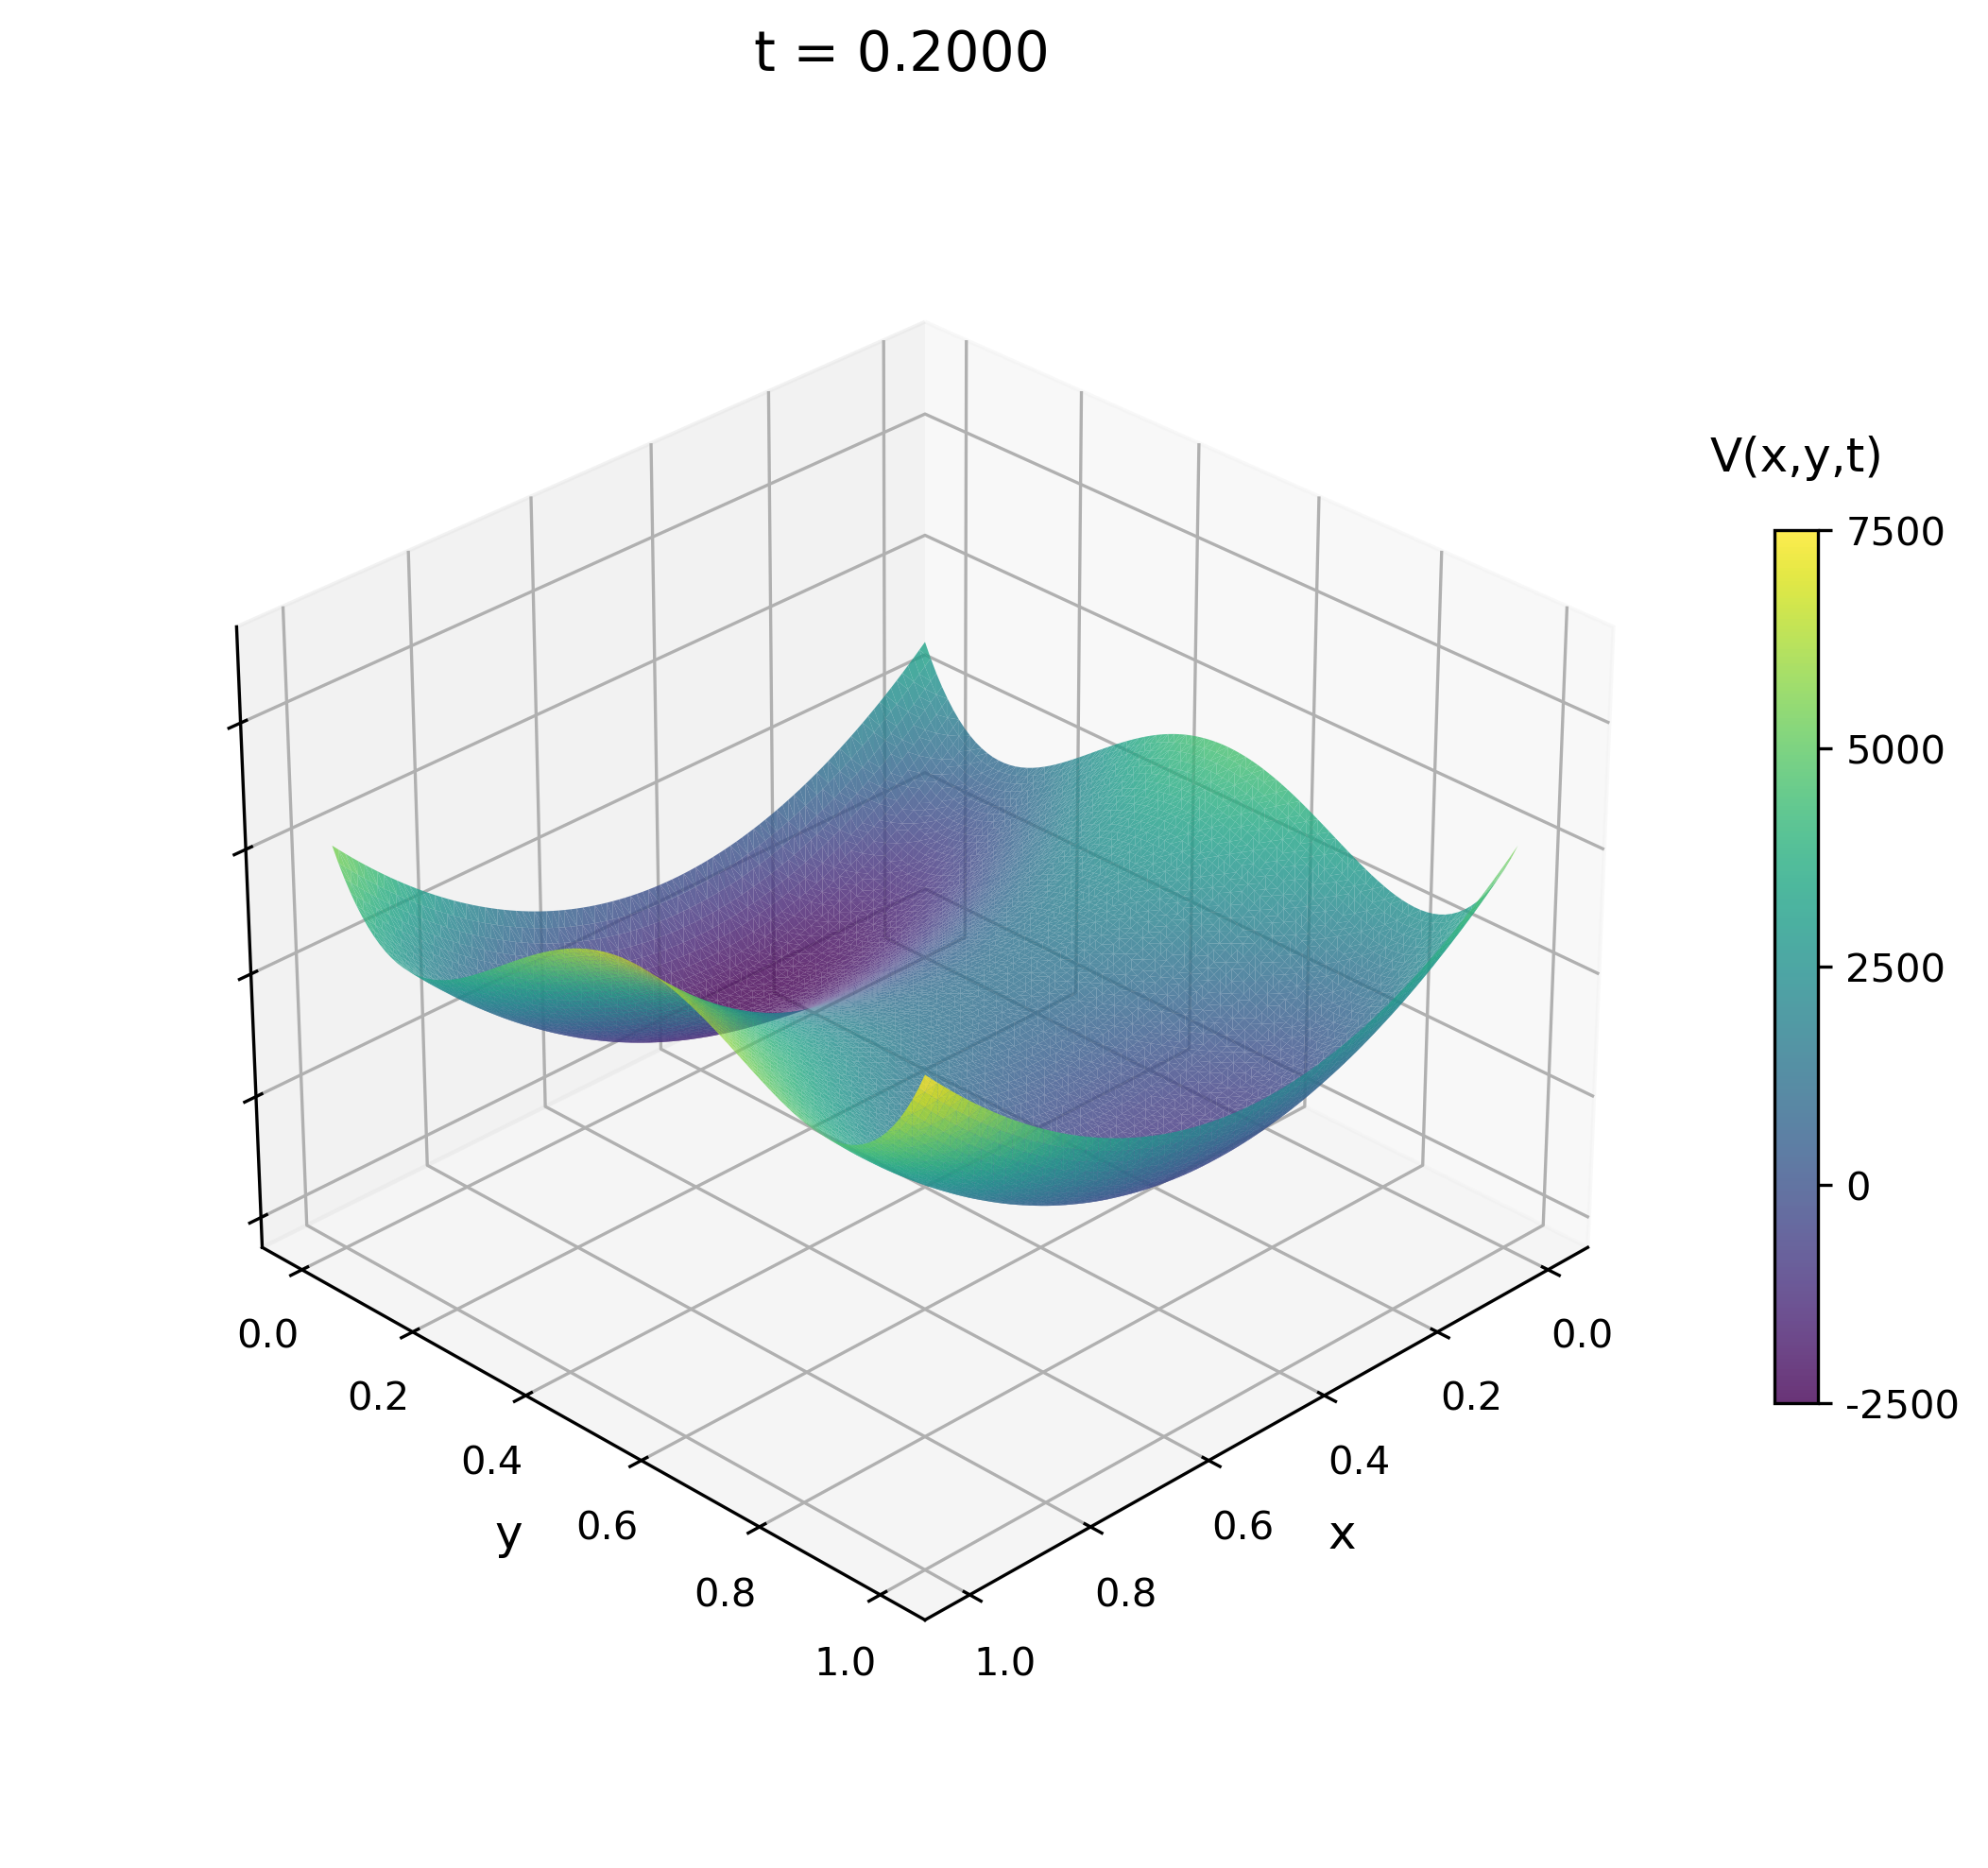
\includegraphics[width=\textwidth, trim=0cm 0cm 0cm 1cm, clip]{figures/potential_frame_0010.png}
    \caption{t = 0.2}
  \end{subfigure}
  \hfill
  \begin{subfigure}[b]{0.3\textwidth}
    \centering
    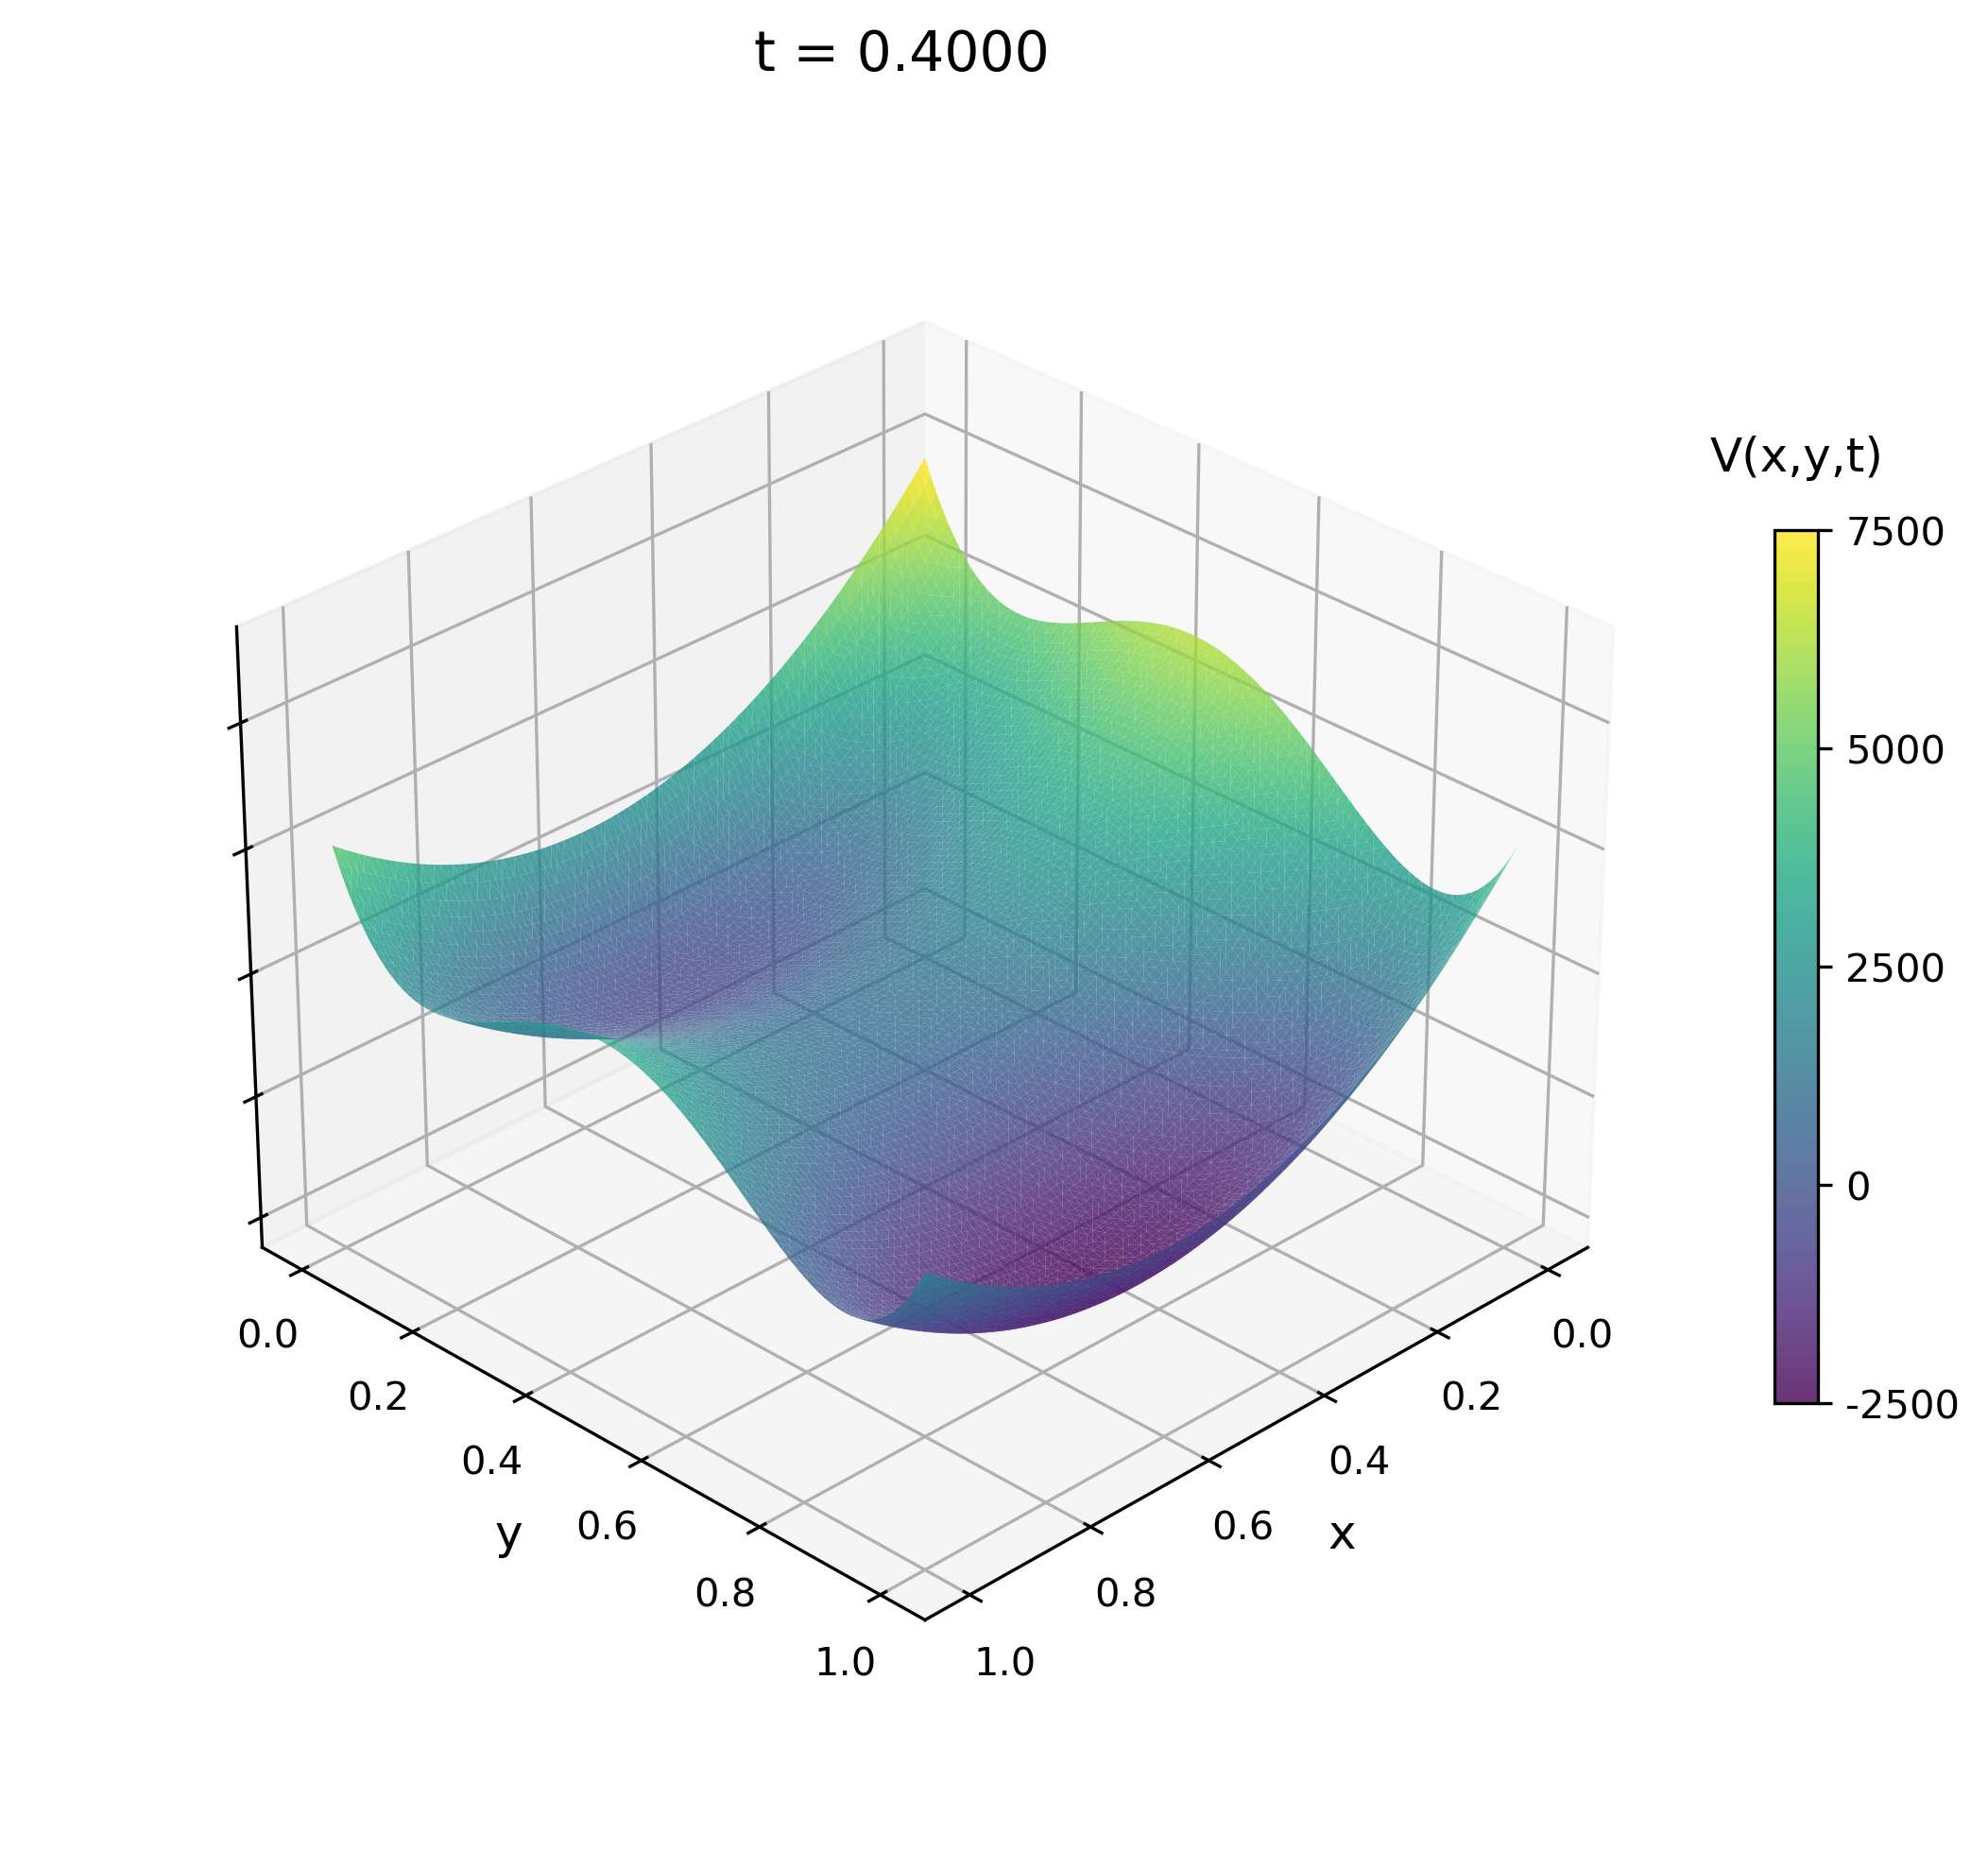
\includegraphics[width=\textwidth, trim=0cm 0cm 0cm 1cm, clip]{figures/potential_frame_0020.png}
    \caption{t = 0.4}
  \end{subfigure}
  
  \vspace{0.5cm}
  
  \begin{subfigure}[b]{0.3\textwidth}
    \centering
    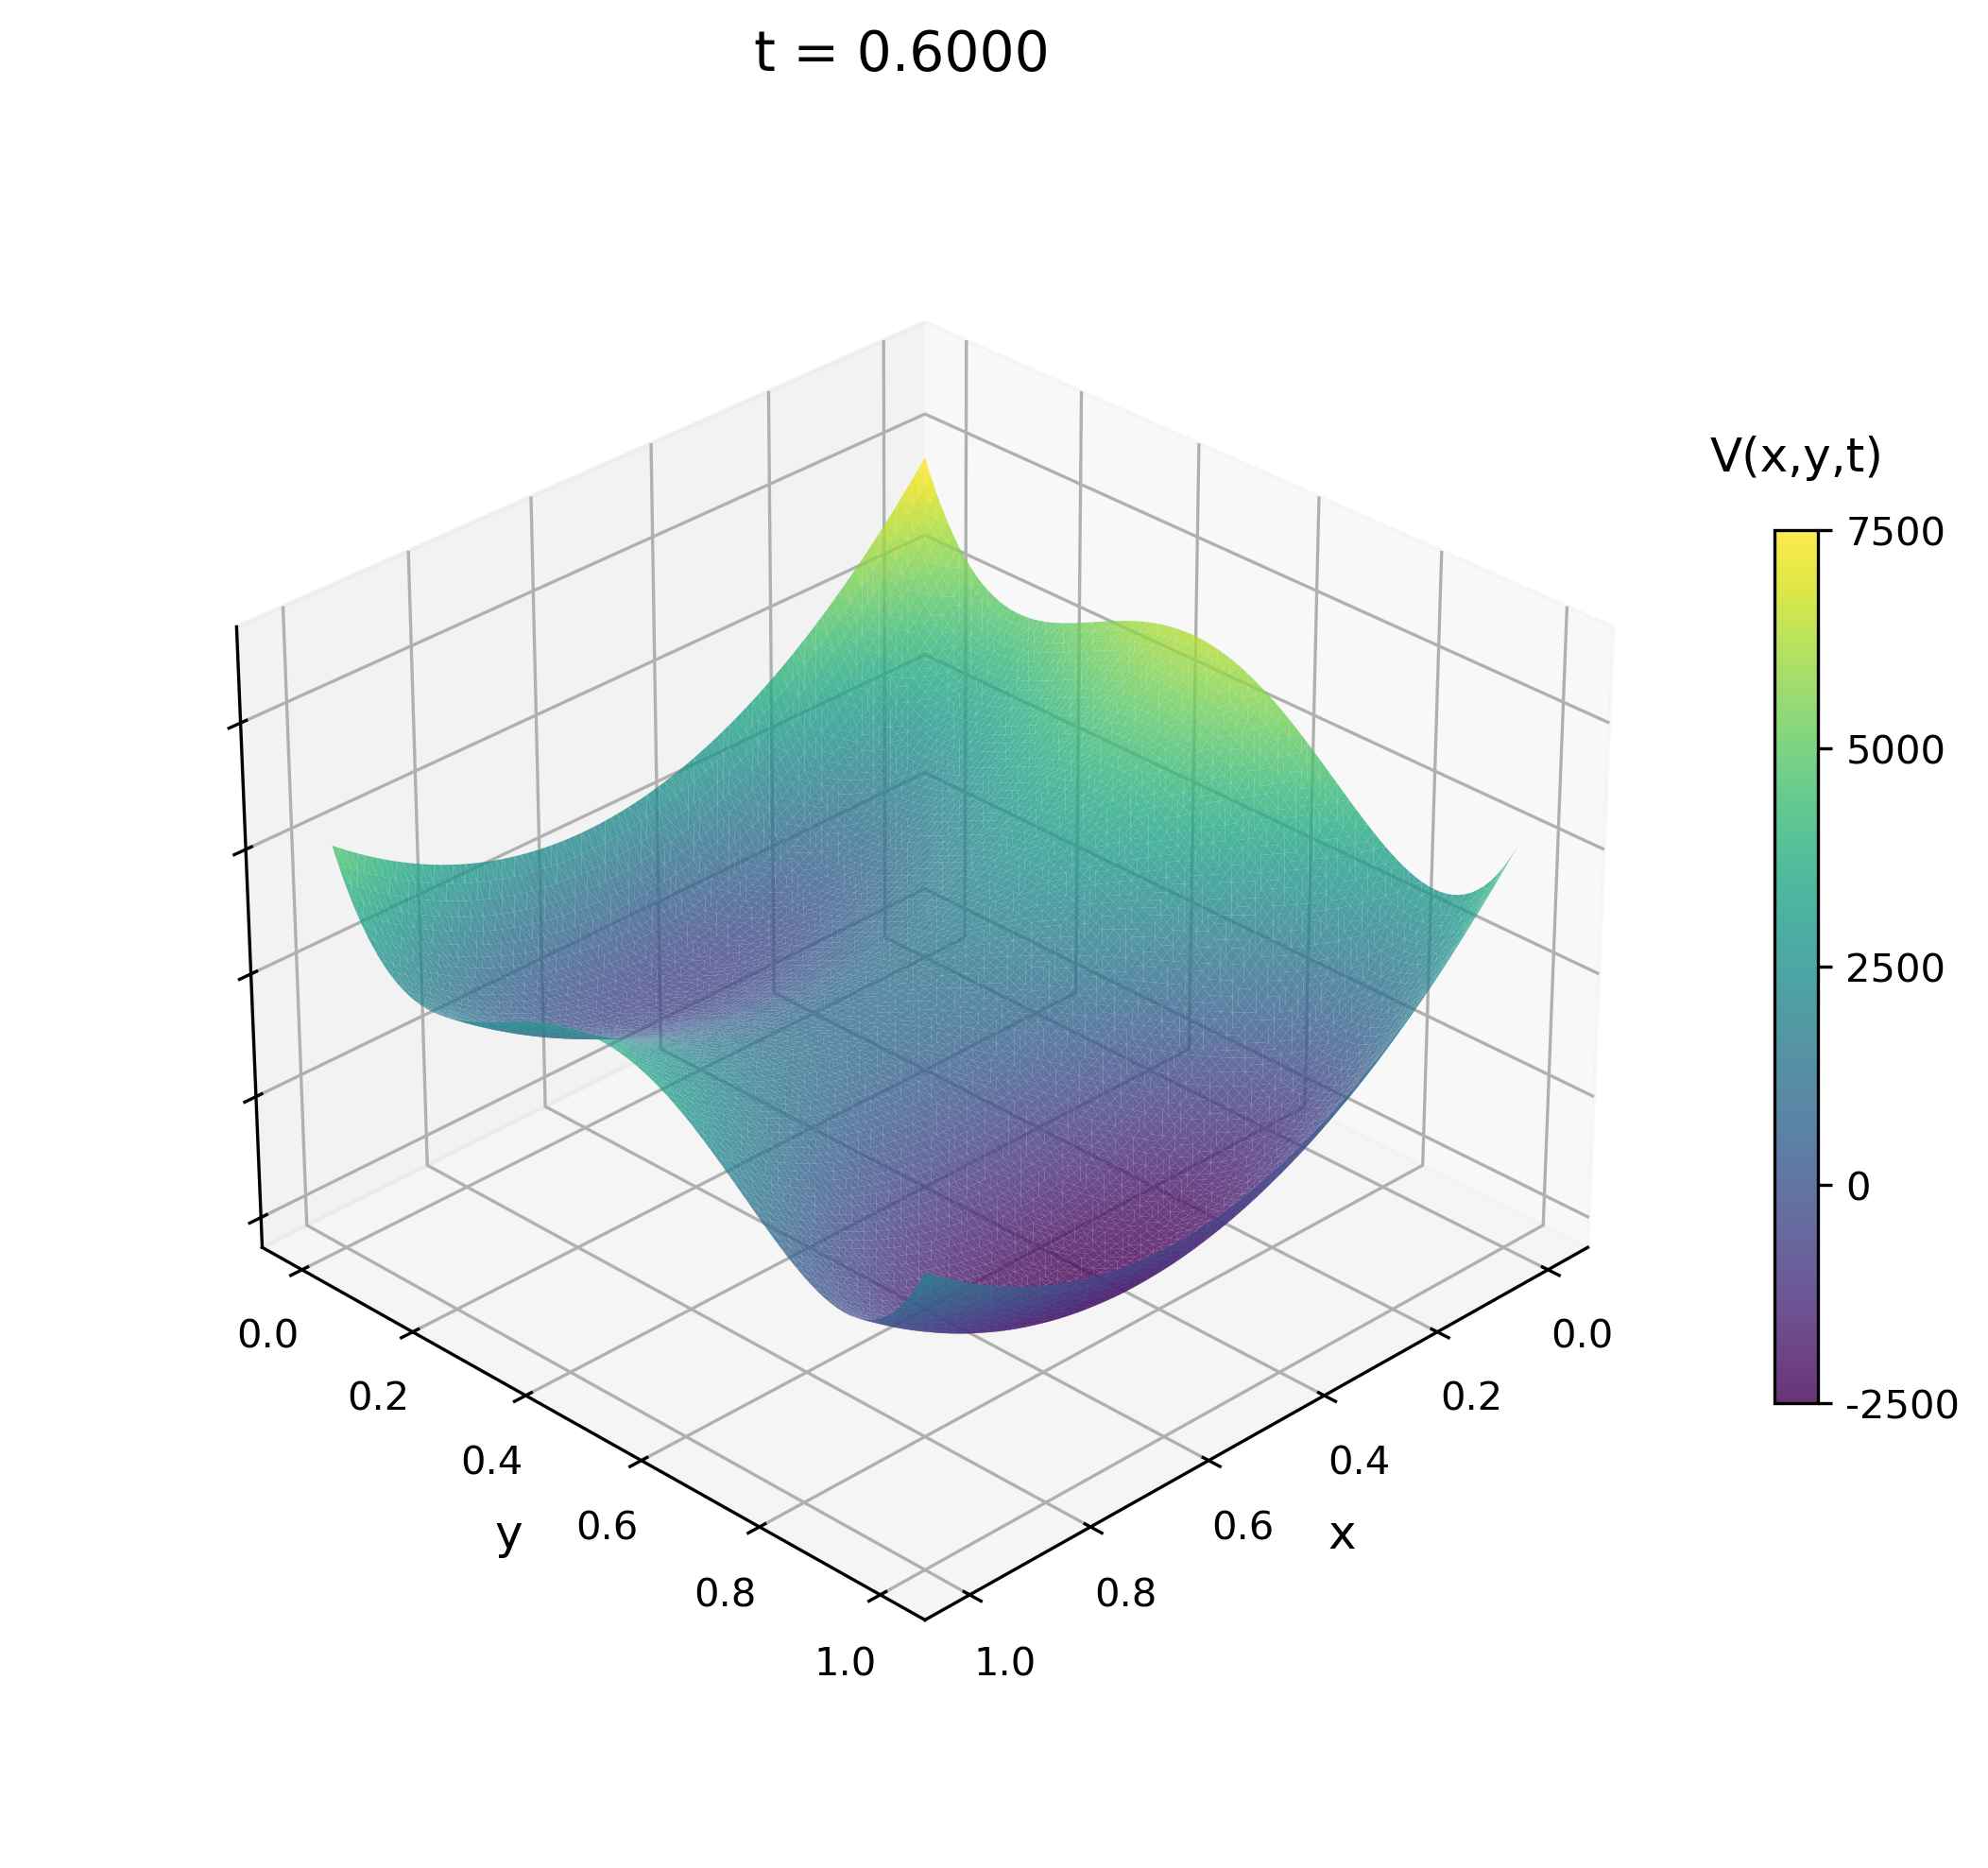
\includegraphics[width=\textwidth, trim=0cm 0cm 0cm 1cm, clip]{figures/potential_frame_0030.png}
    \caption{t = 0.6}
  \end{subfigure}
  \hfill
  \begin{subfigure}[b]{0.3\textwidth}
    \centering
    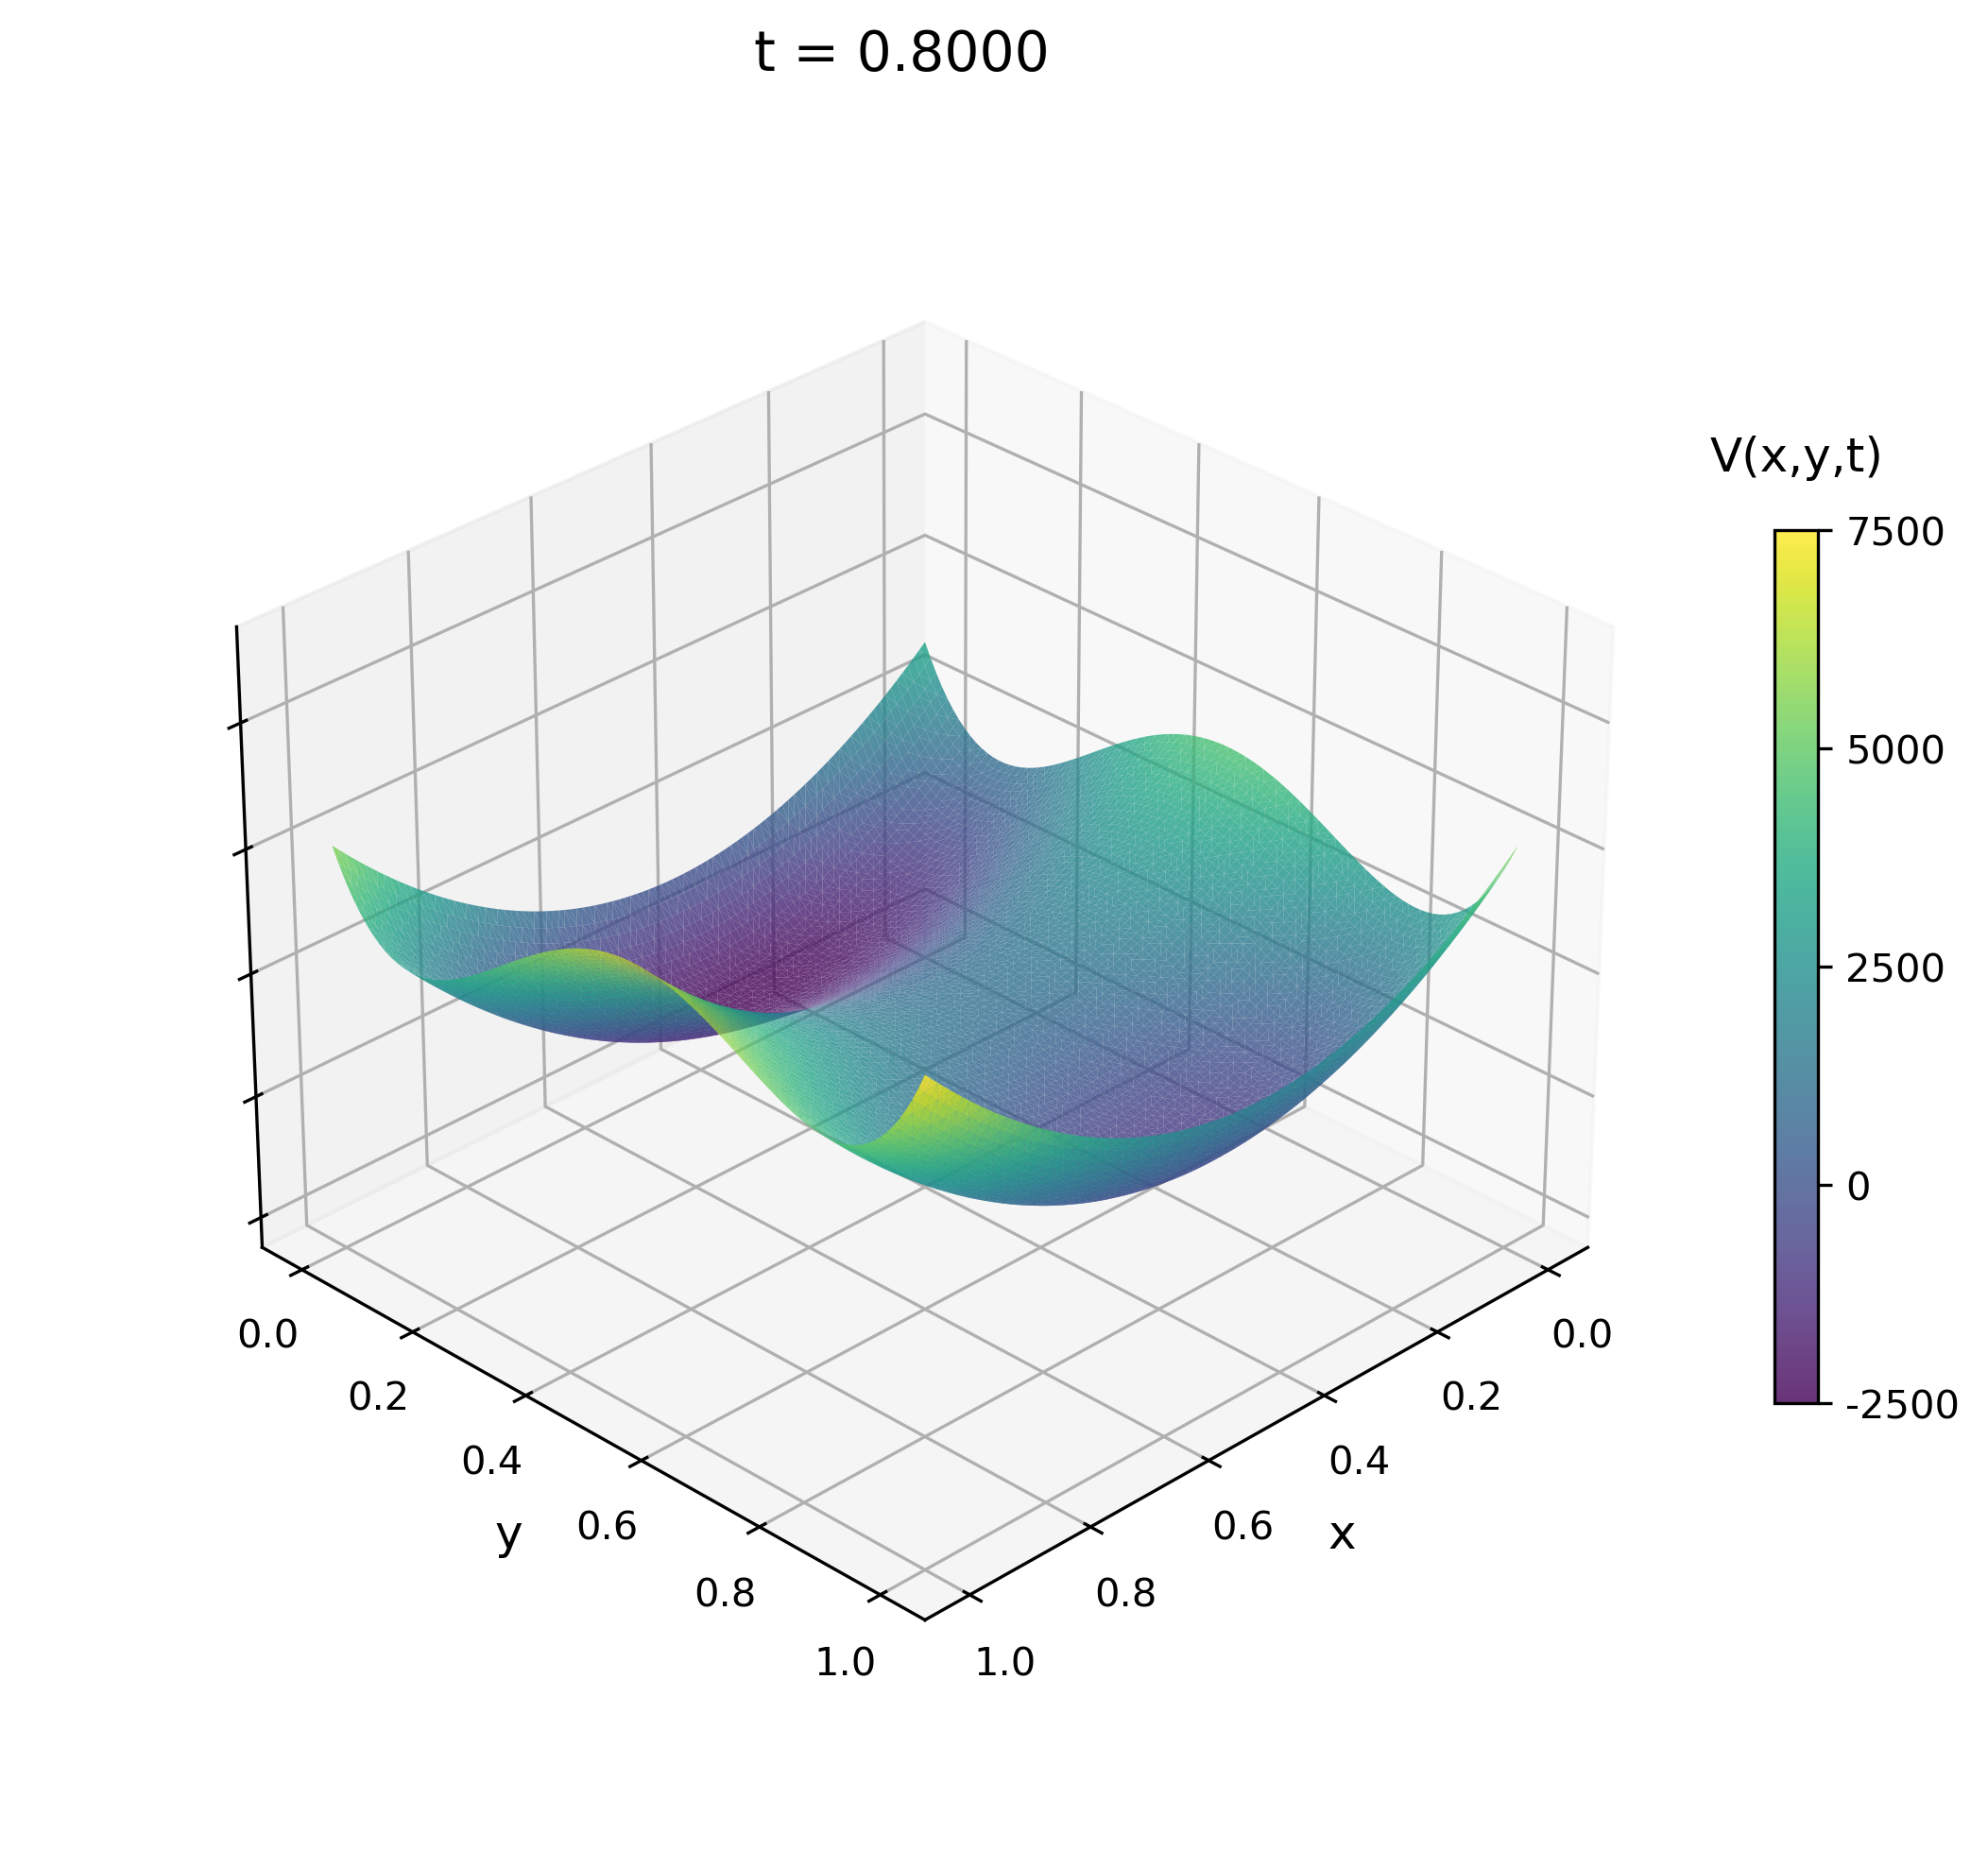
\includegraphics[width=\textwidth, trim=0cm 0cm 0cm 1cm, clip]{figures/potential_frame_0040.png}
    \caption{t = 0.8}
  \end{subfigure}
  \hfill
  \begin{subfigure}[b]{0.3\textwidth}
    \centering
    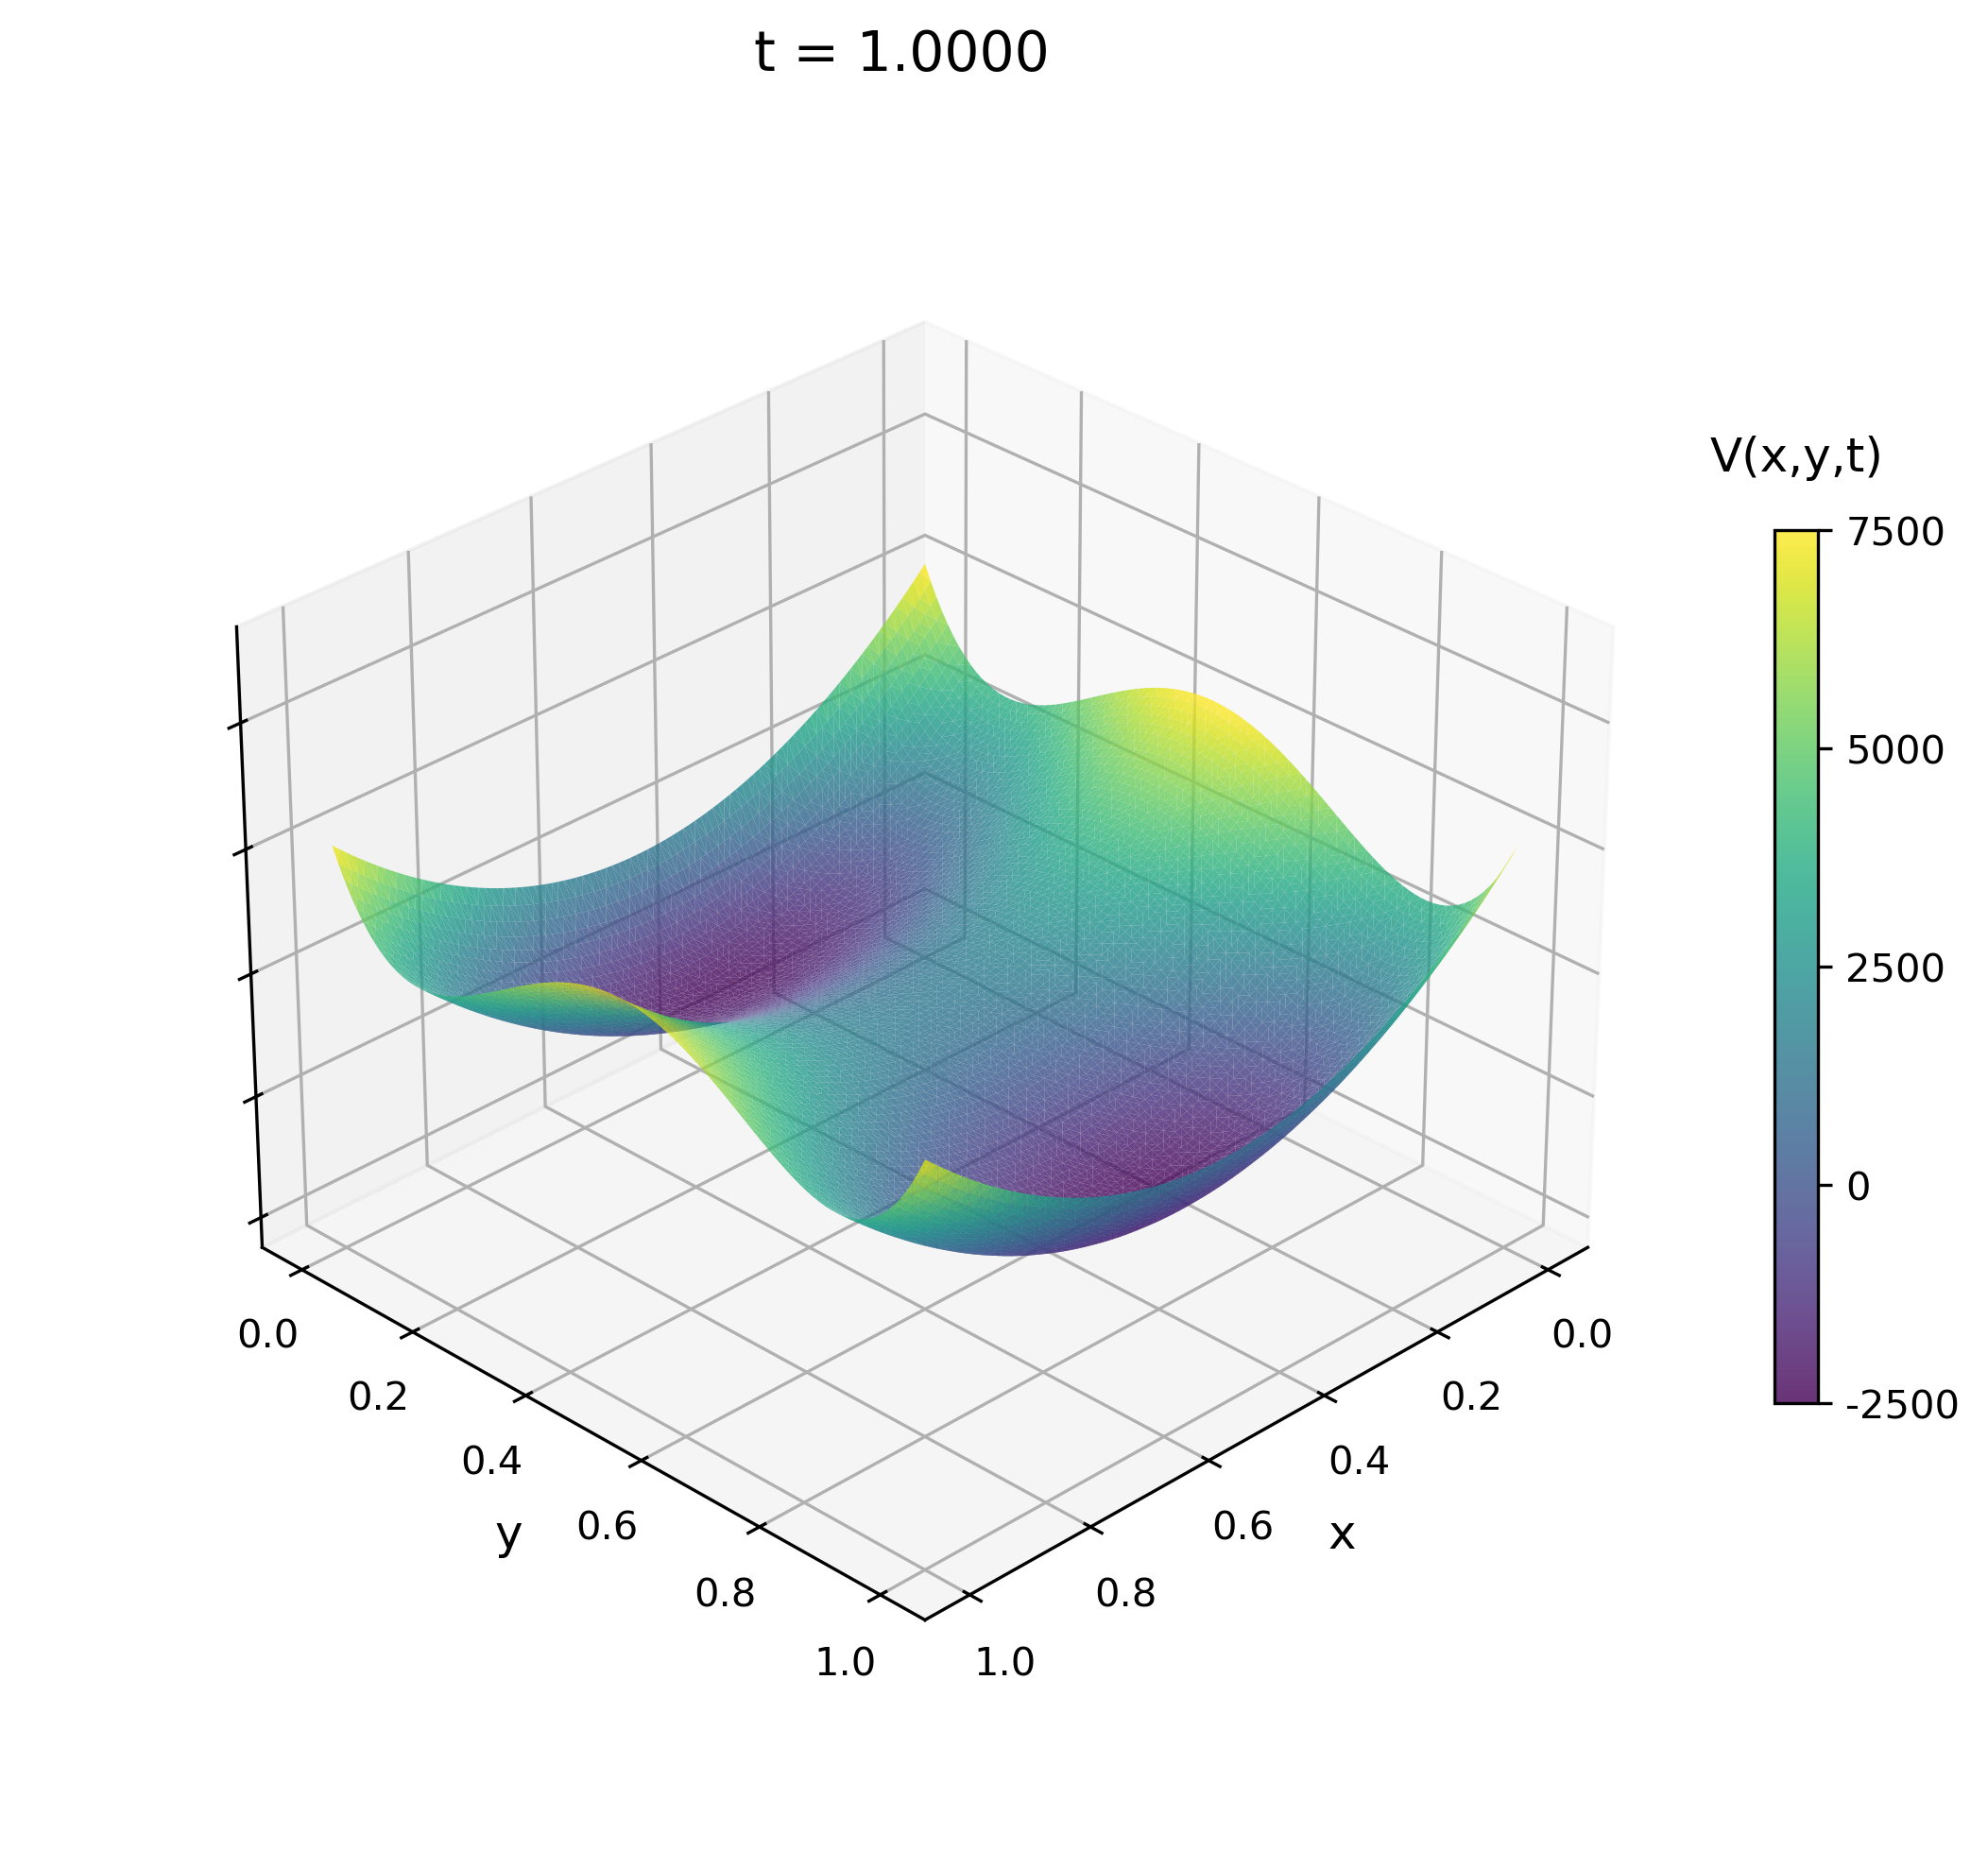
\includegraphics[width=\textwidth, trim=0cm 0cm 0cm 1cm, clip]{figures/potential_frame_0050.png}
    \caption{t = 1.0}
  \end{subfigure}
  \caption{Time evolution of the solution of the Schrödinger equation with the time-dependent model potential, obtained with the PINN.}
  \label{fig:potential_evolution}
\end{figure}




\begin{figure}[h]
  \centering
  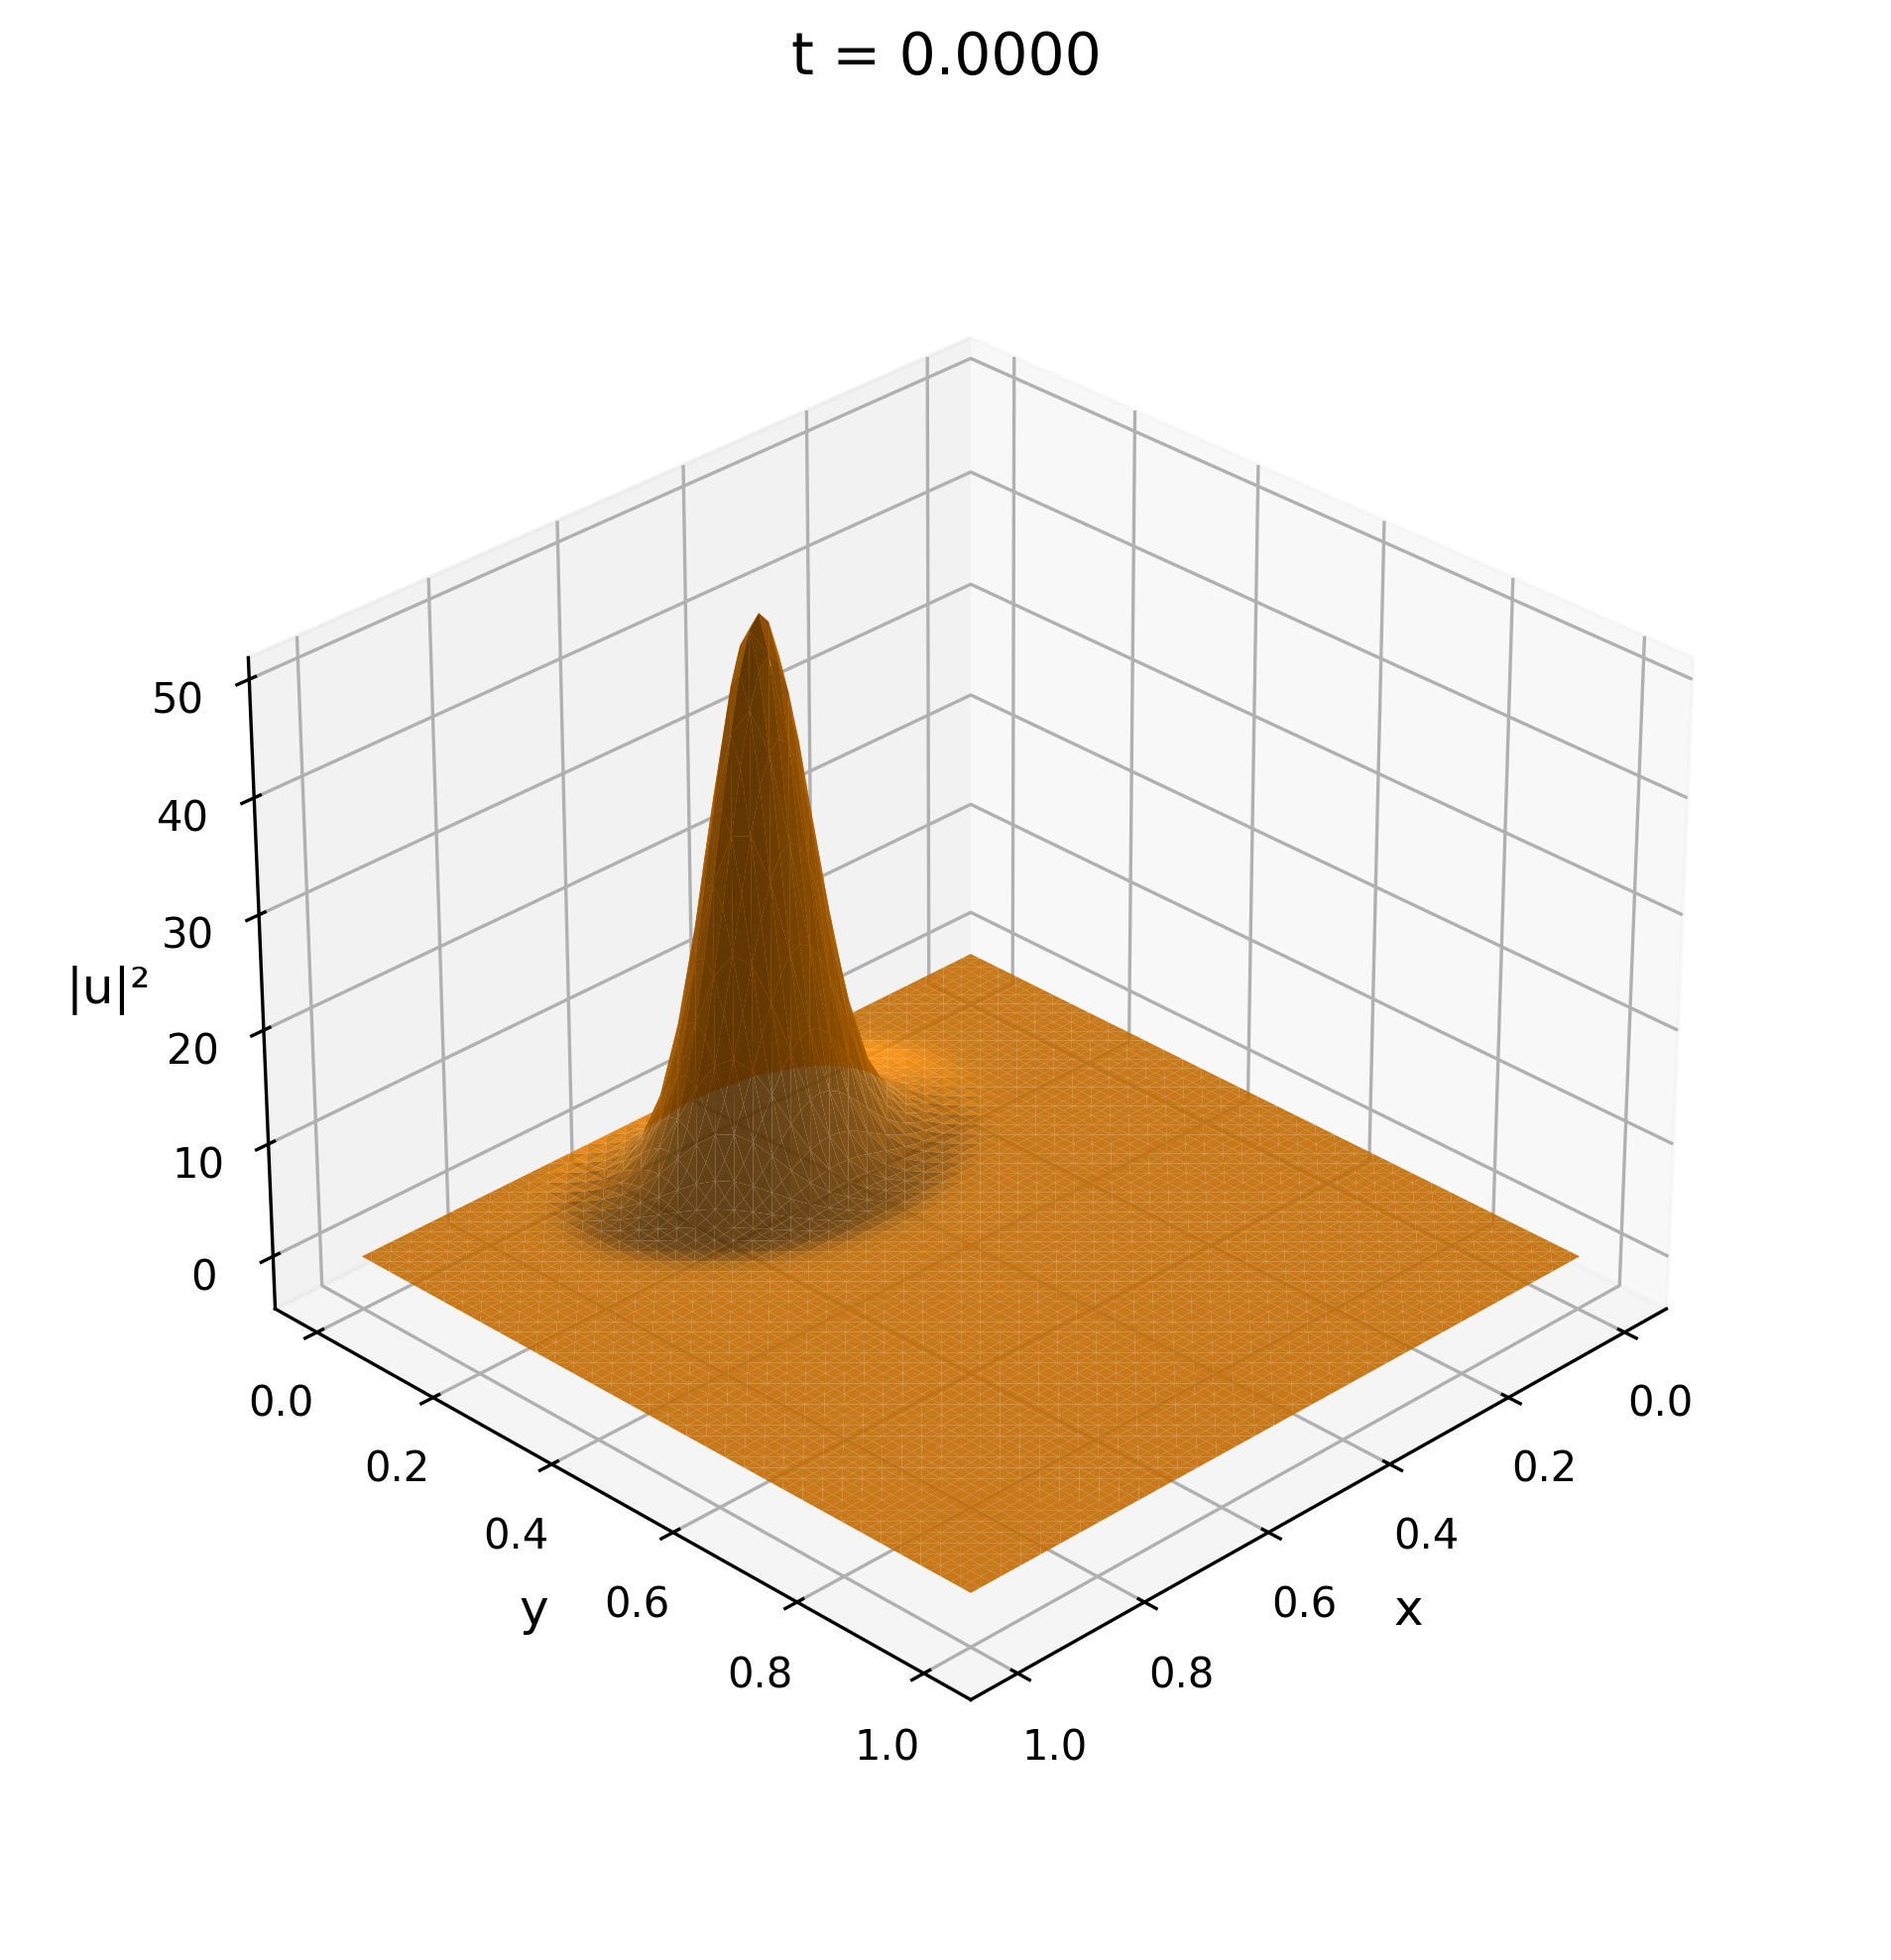
\includegraphics[width=0.7\textwidth]{figures/potential_initial_state_3d.png}
  \caption{Initial State with Potential}
  \label{fig:initial_state_with_potential}
\end{figure}



\begin{figure}[h]
  \centering
  \begin{subfigure}[b]{0.3\textwidth}
    \centering
    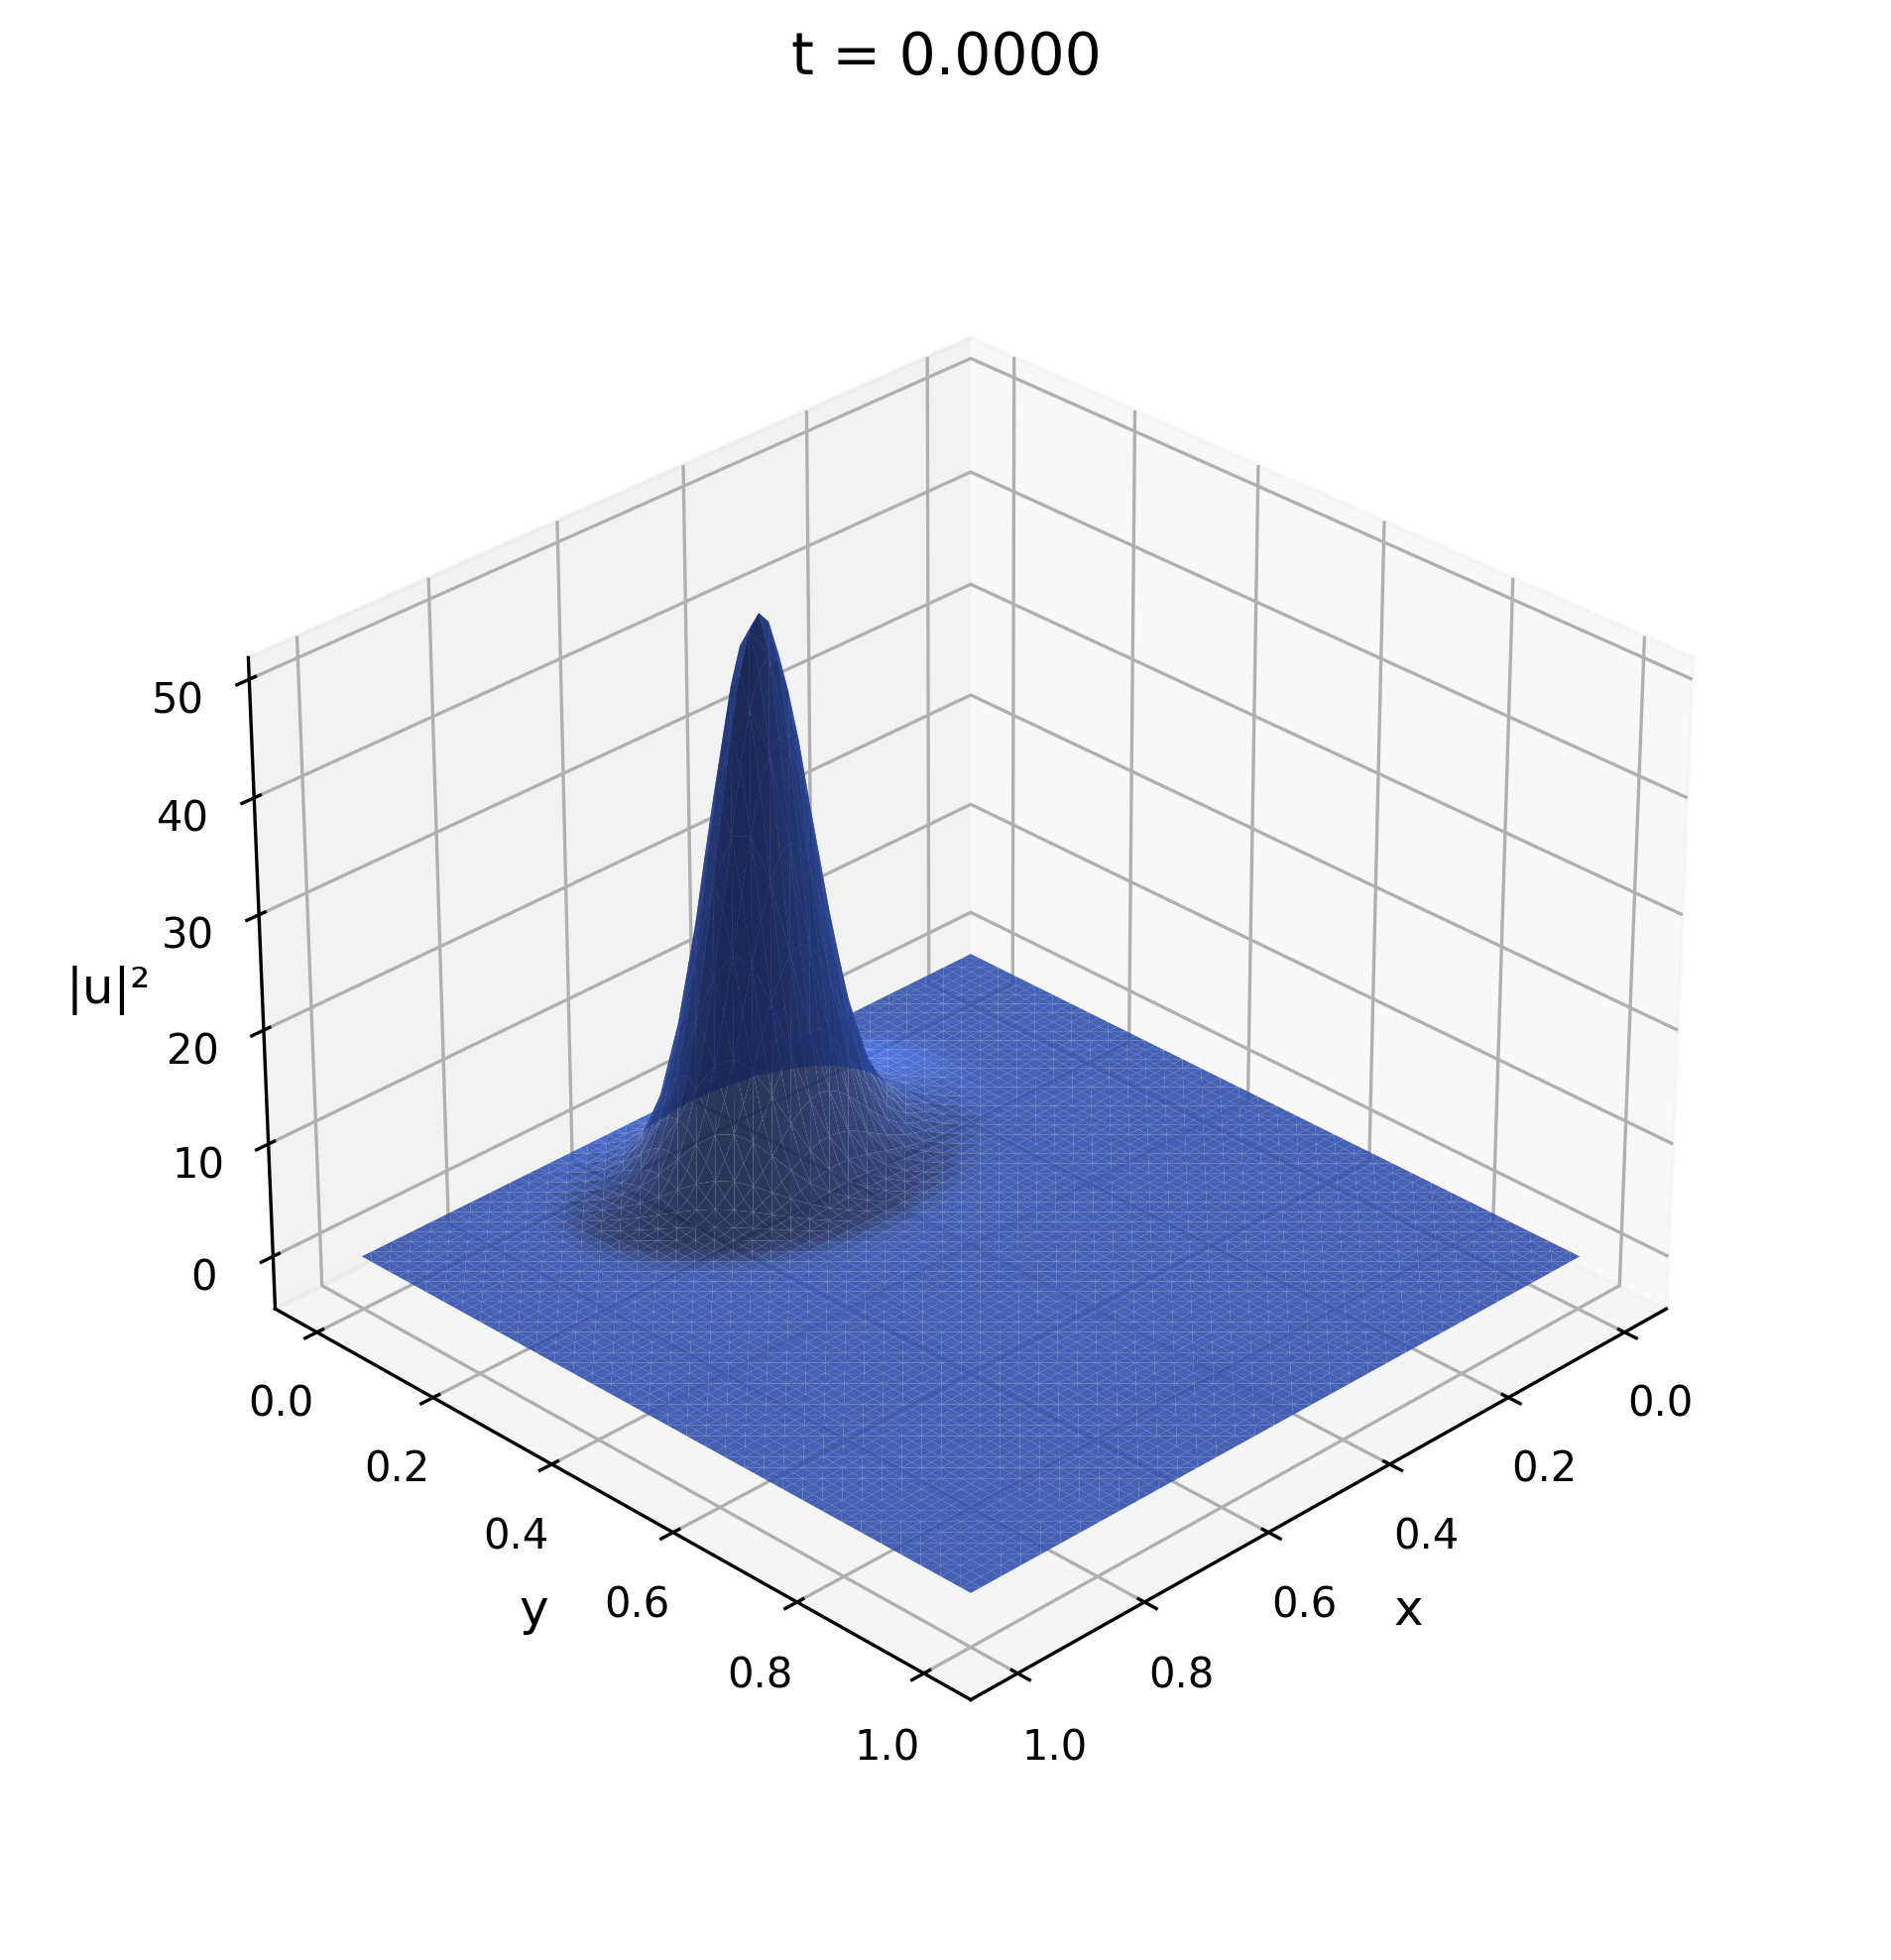
\includegraphics[width=\textwidth, trim=0cm 0cm 0cm 1cm, clip]{figures/fem_potential_frame_0000.png}
    \caption{t = 0.0}
  \end{subfigure}
  \hfill
  \begin{subfigure}[b]{0.3\textwidth}
    \centering
    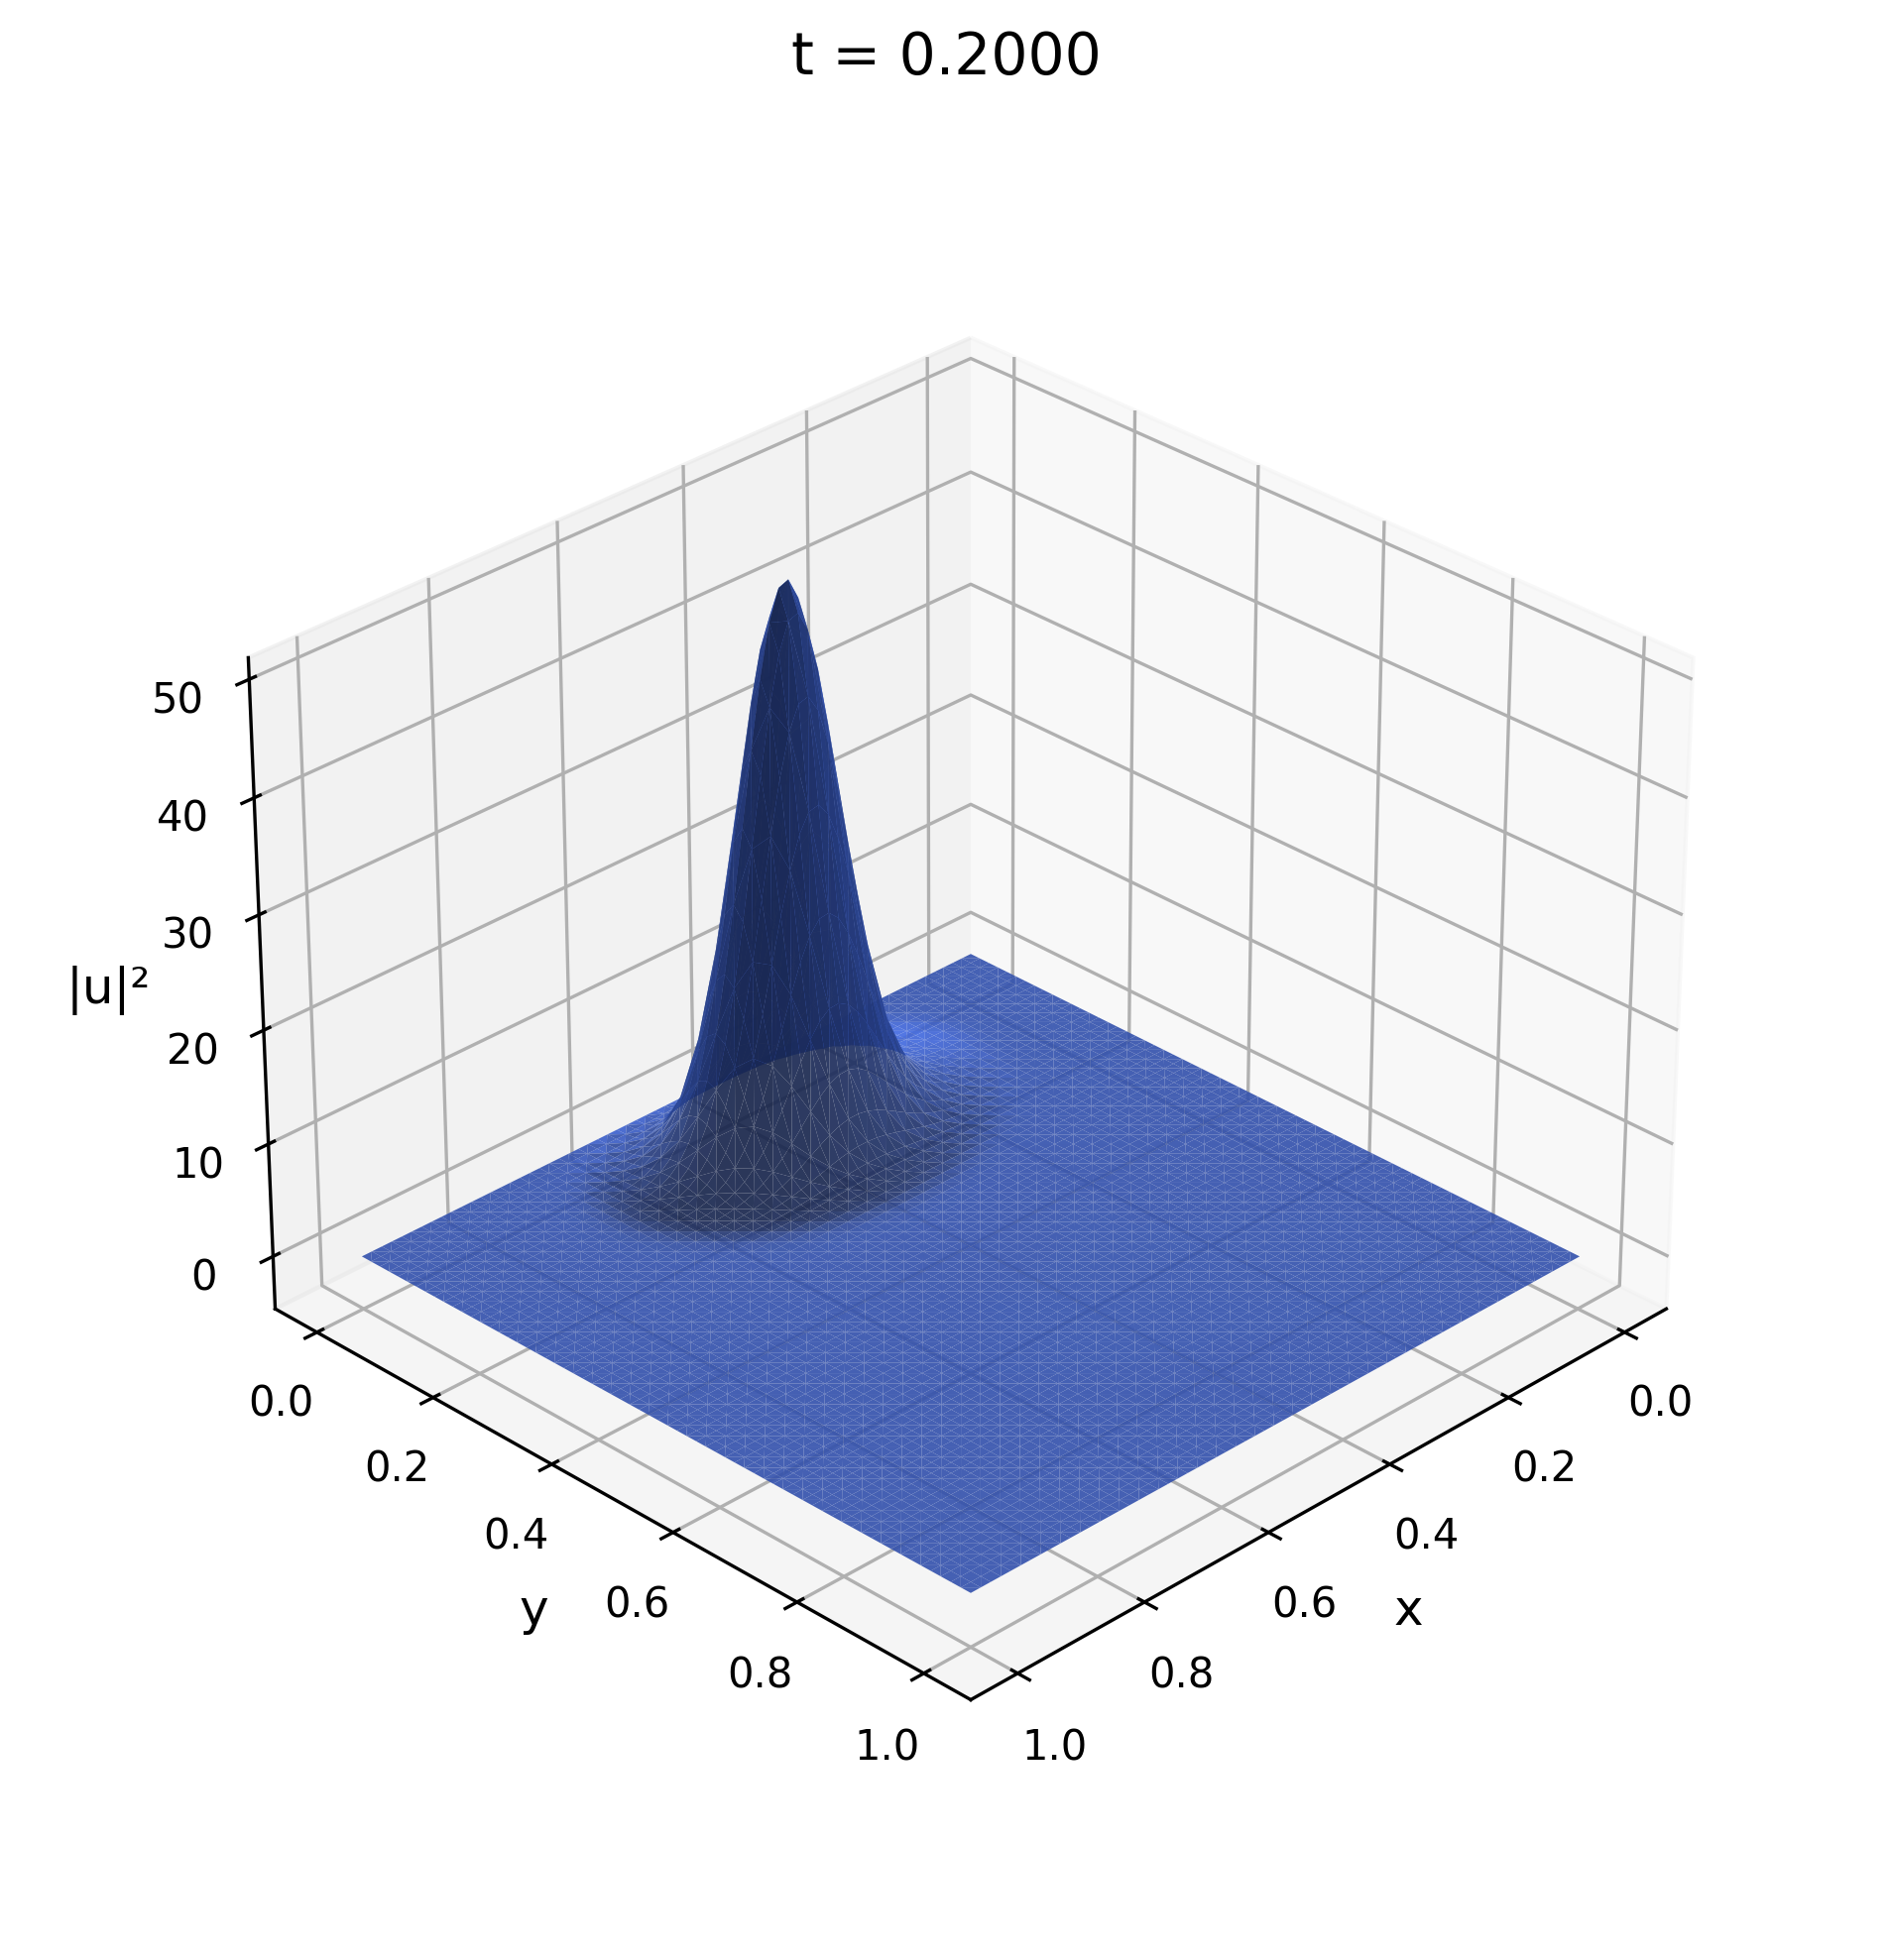
\includegraphics[width=\textwidth, trim=0cm 0cm 0cm 1cm, clip]{figures/fem_potential_frame_0020.png}
    \caption{t = 0.2}
  \end{subfigure}
  \hfill
  \begin{subfigure}[b]{0.3\textwidth}
    \centering
    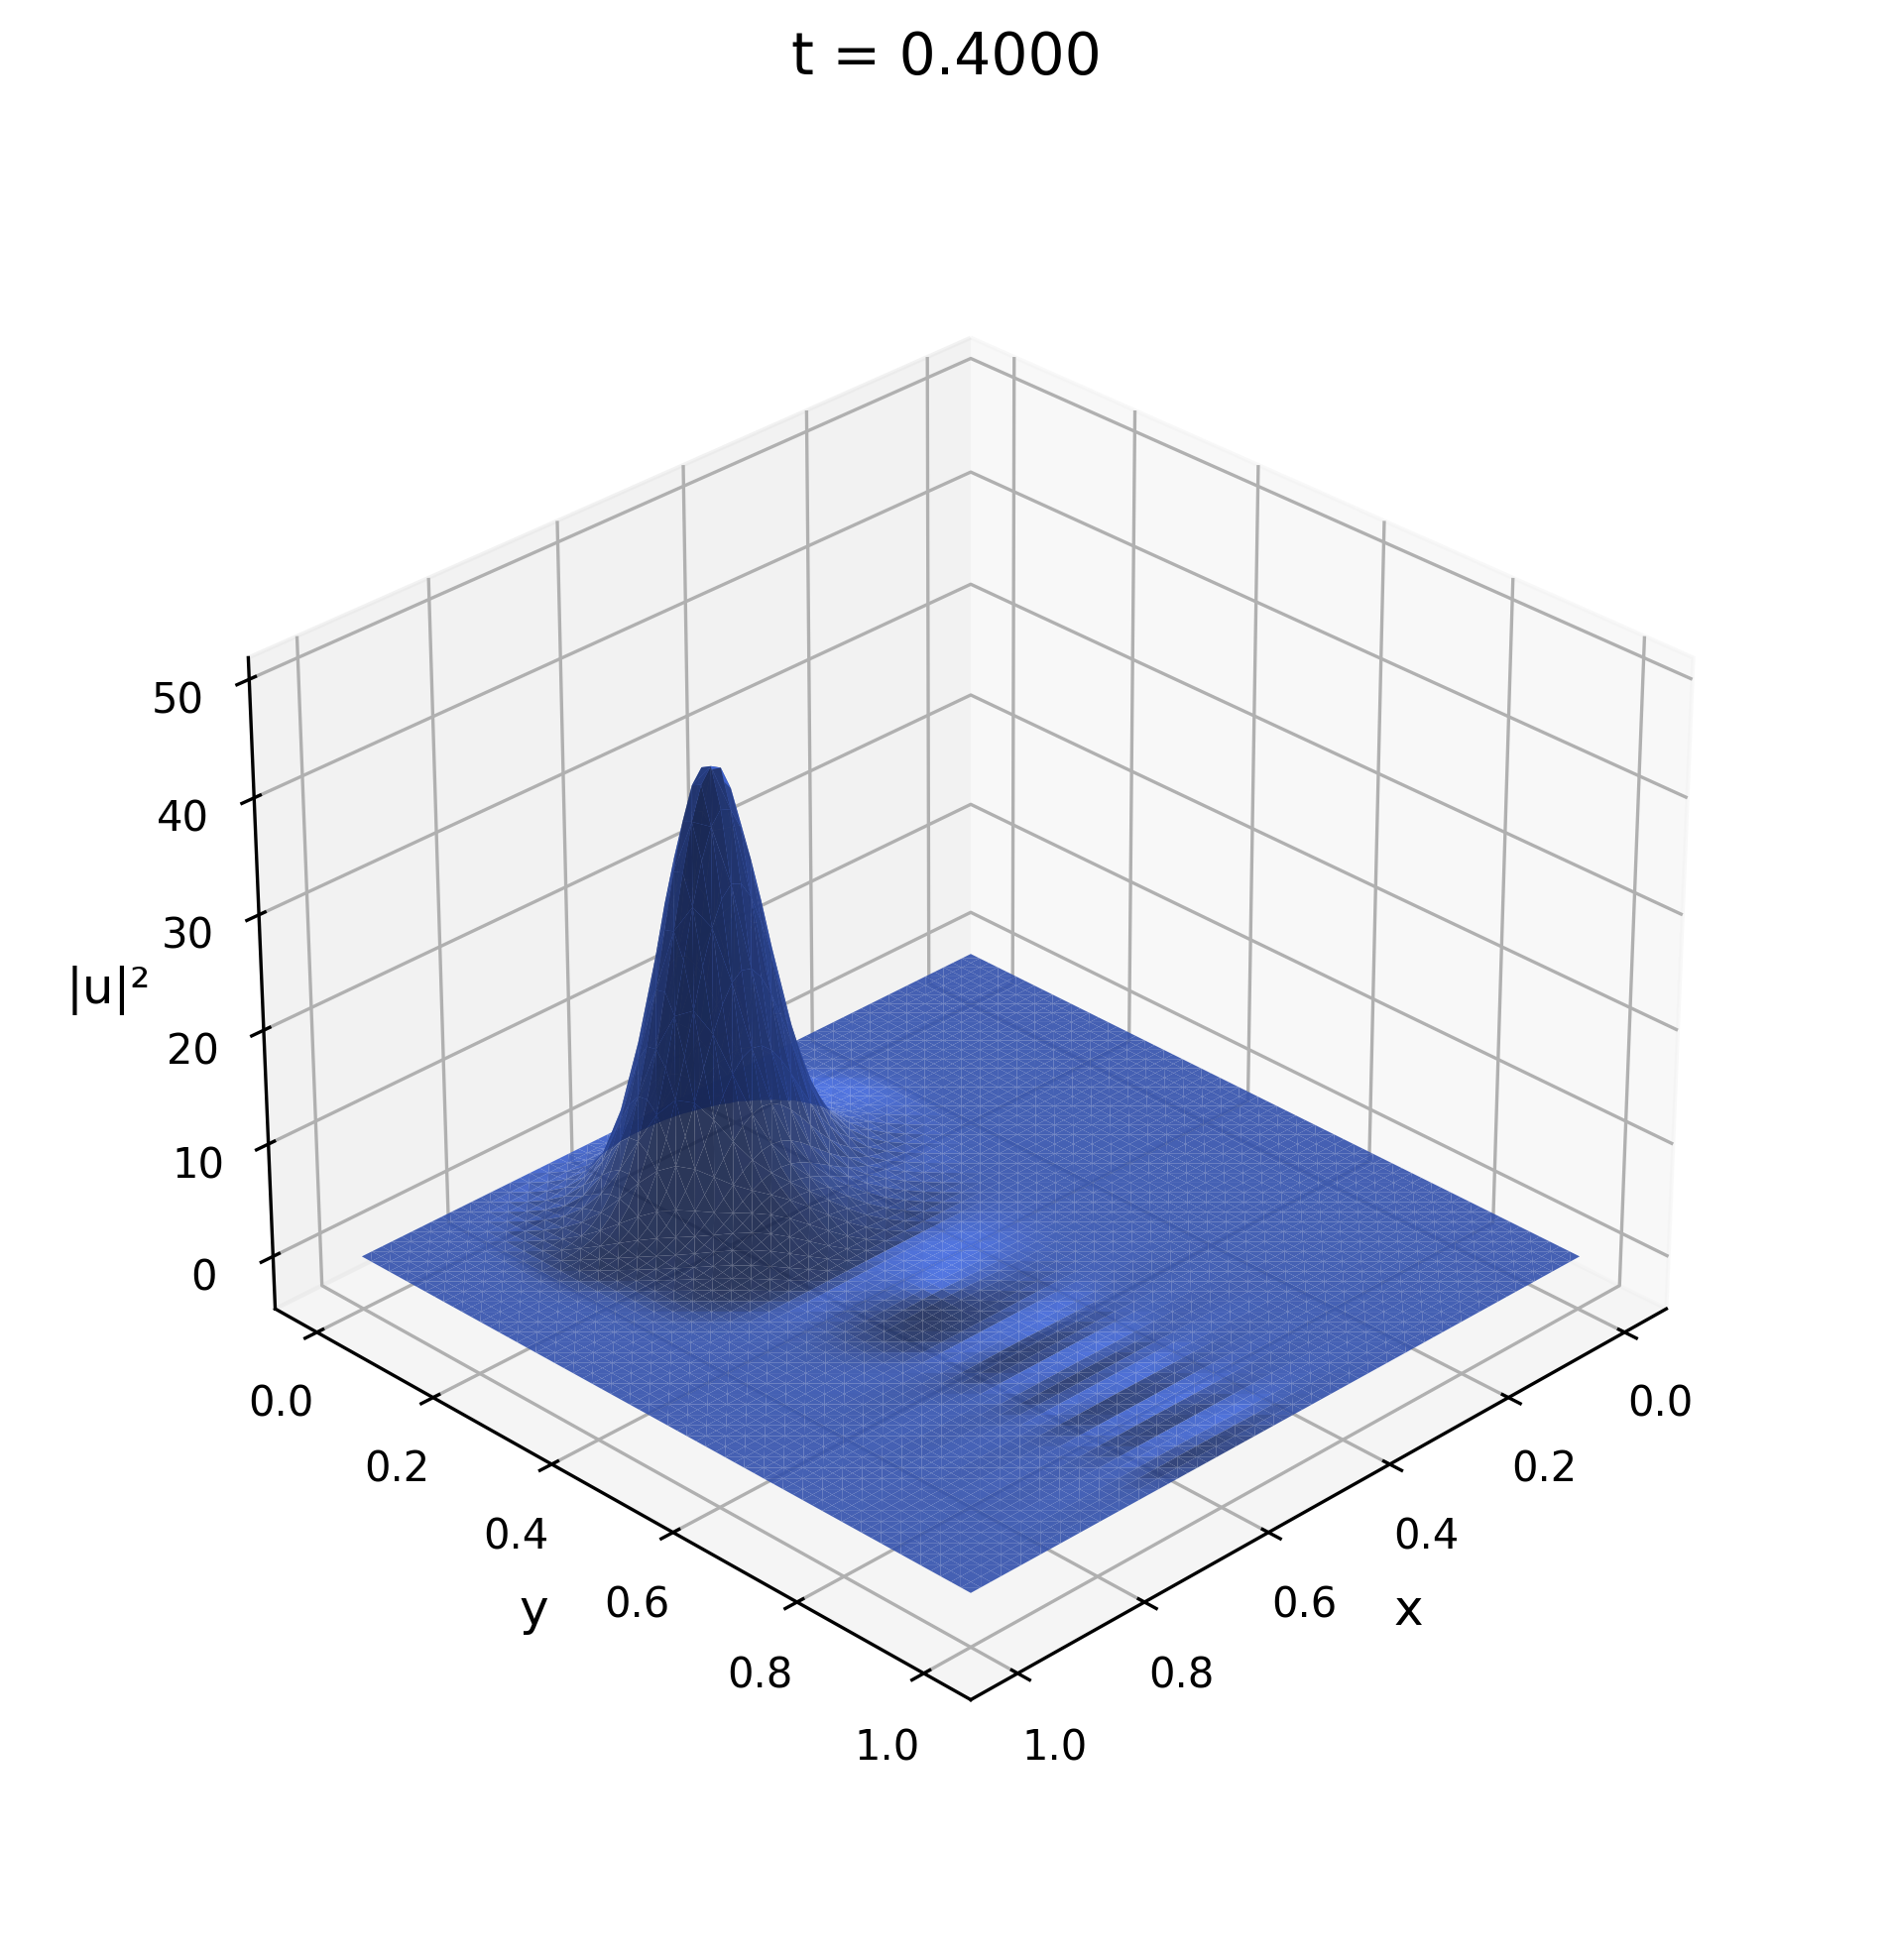
\includegraphics[width=\textwidth, trim=0cm 0cm 0cm 1cm, clip]{figures/fem_potential_frame_0040.png}
    \caption{t = 0.4}
  \end{subfigure}
  
  \vspace{0.5cm}
  
  \begin{subfigure}[b]{0.3\textwidth}
    \centering
    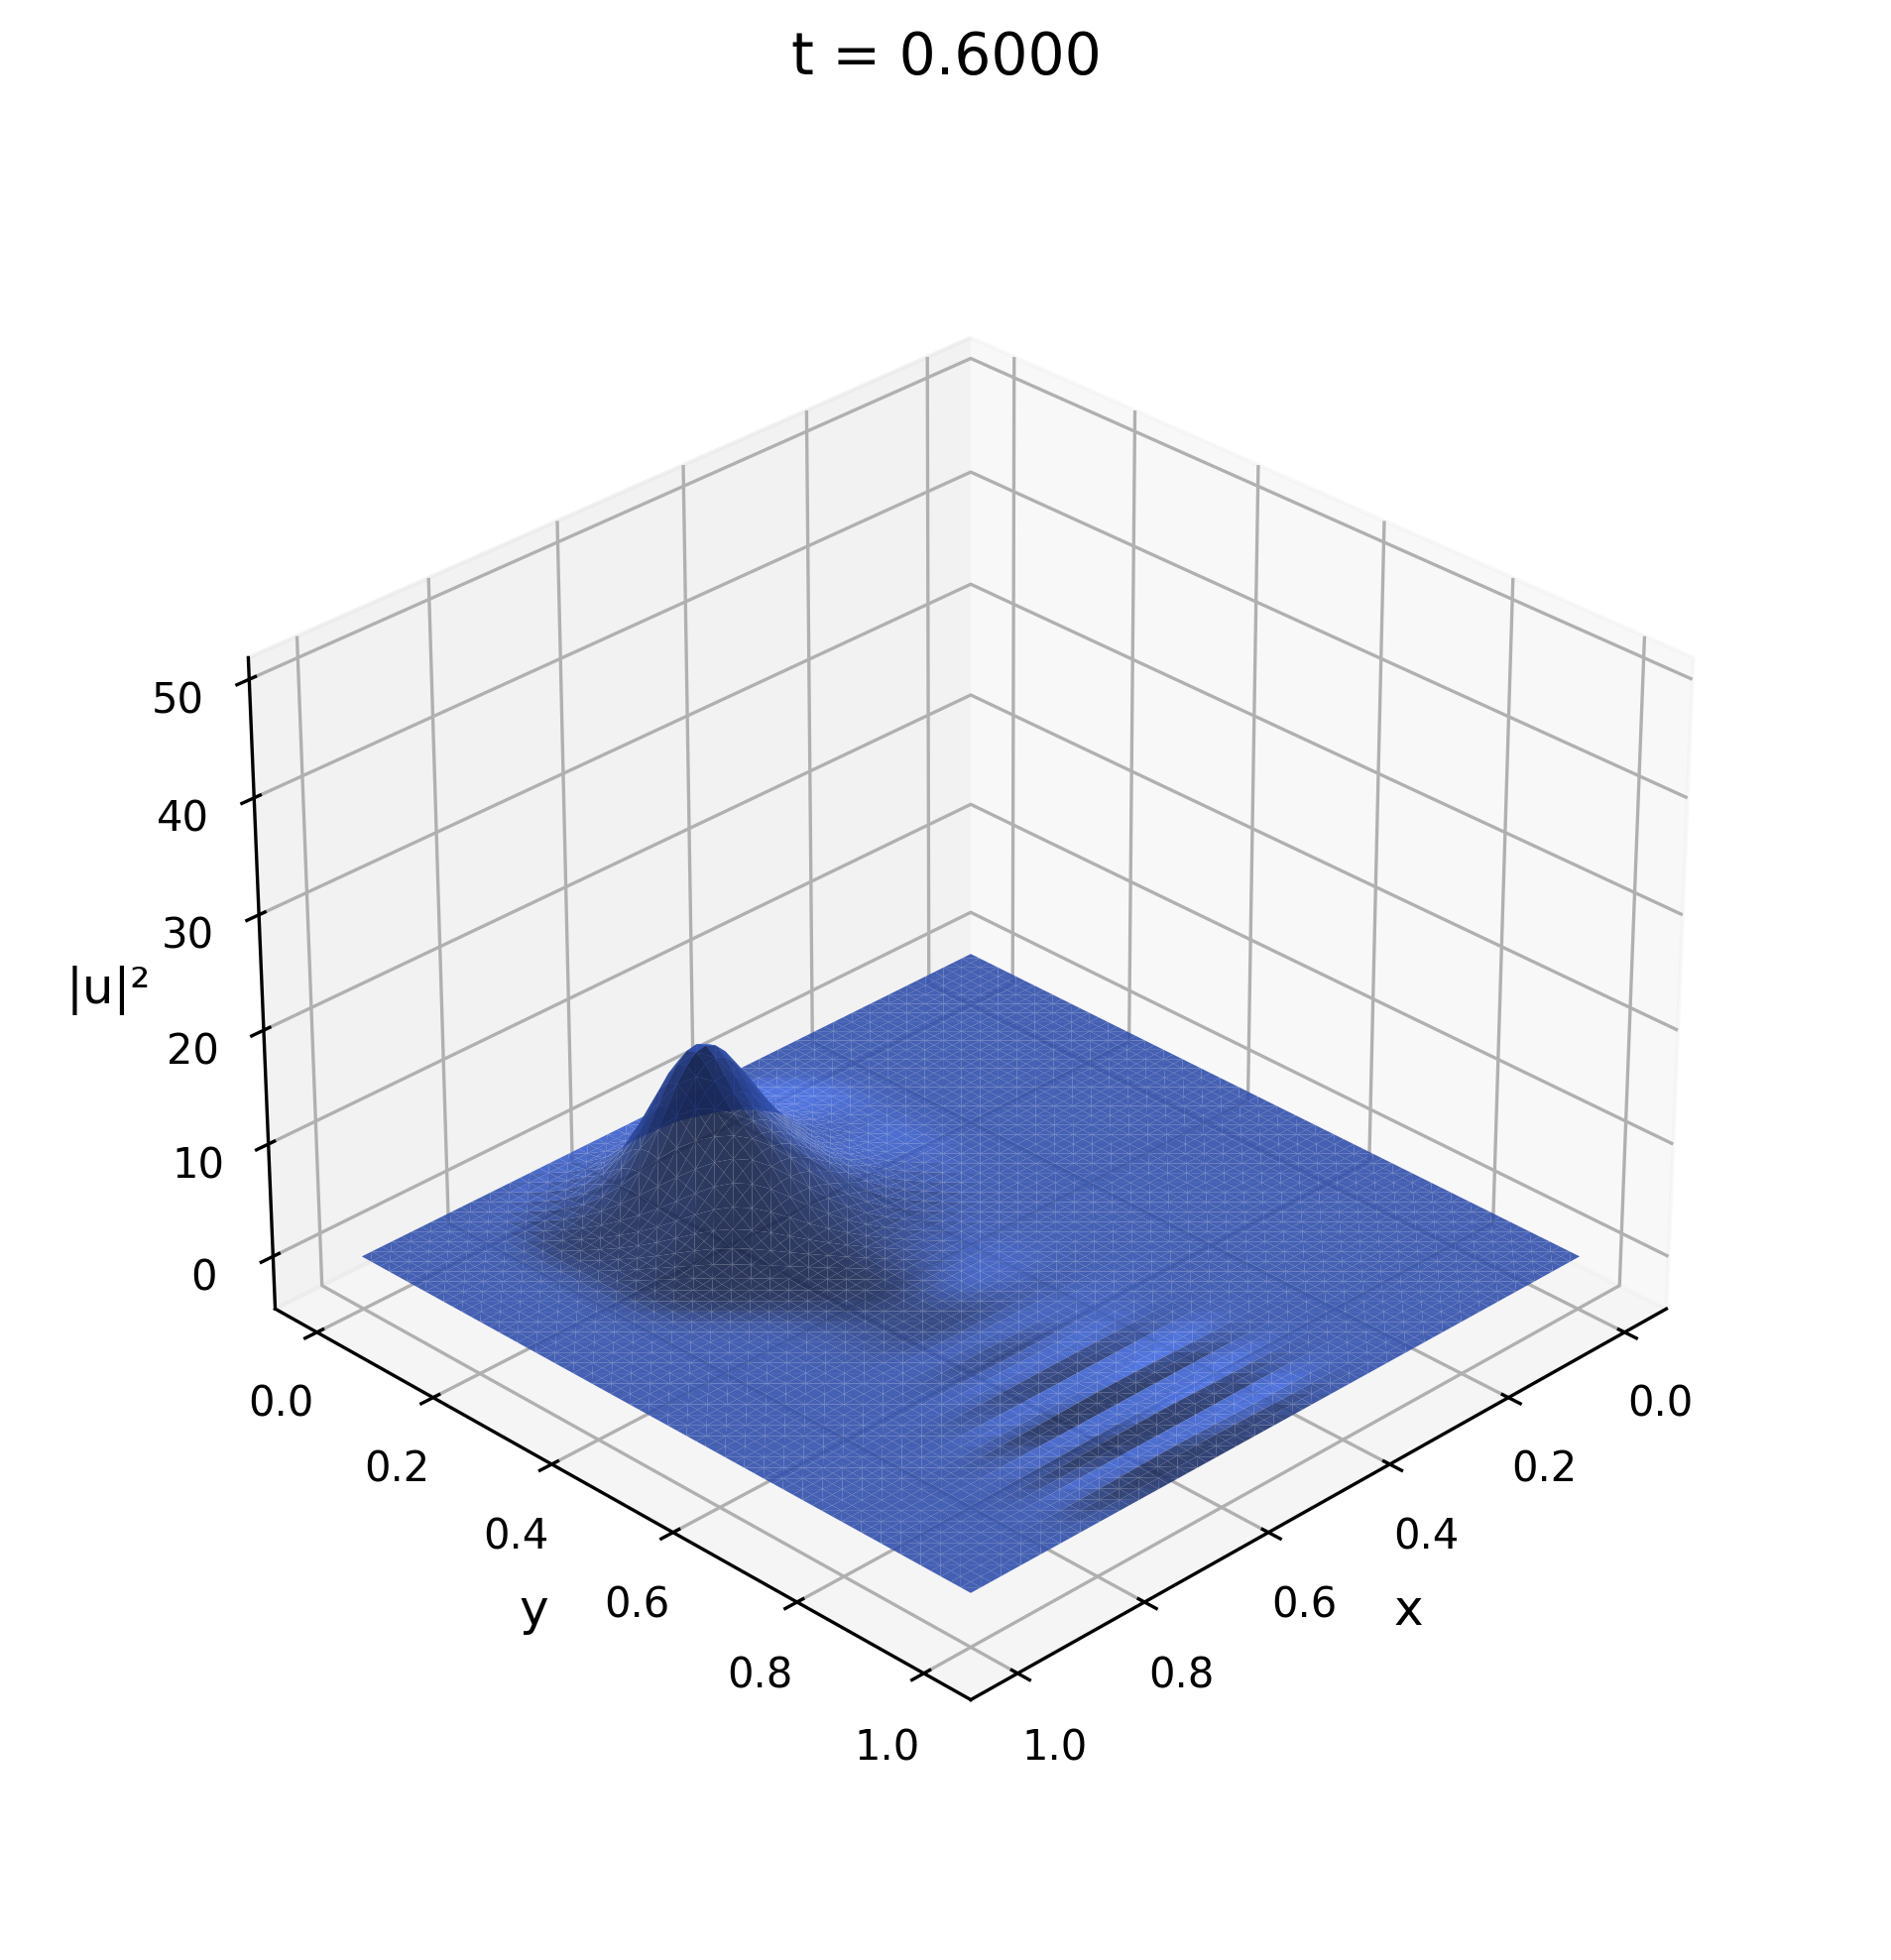
\includegraphics[width=\textwidth, trim=0cm 0cm 0cm 1cm, clip]{figures/fem_potential_frame_0060.png}
    \caption{t = 0.6}
  \end{subfigure}
  \hfill
  \begin{subfigure}[b]{0.3\textwidth}
    \centering
    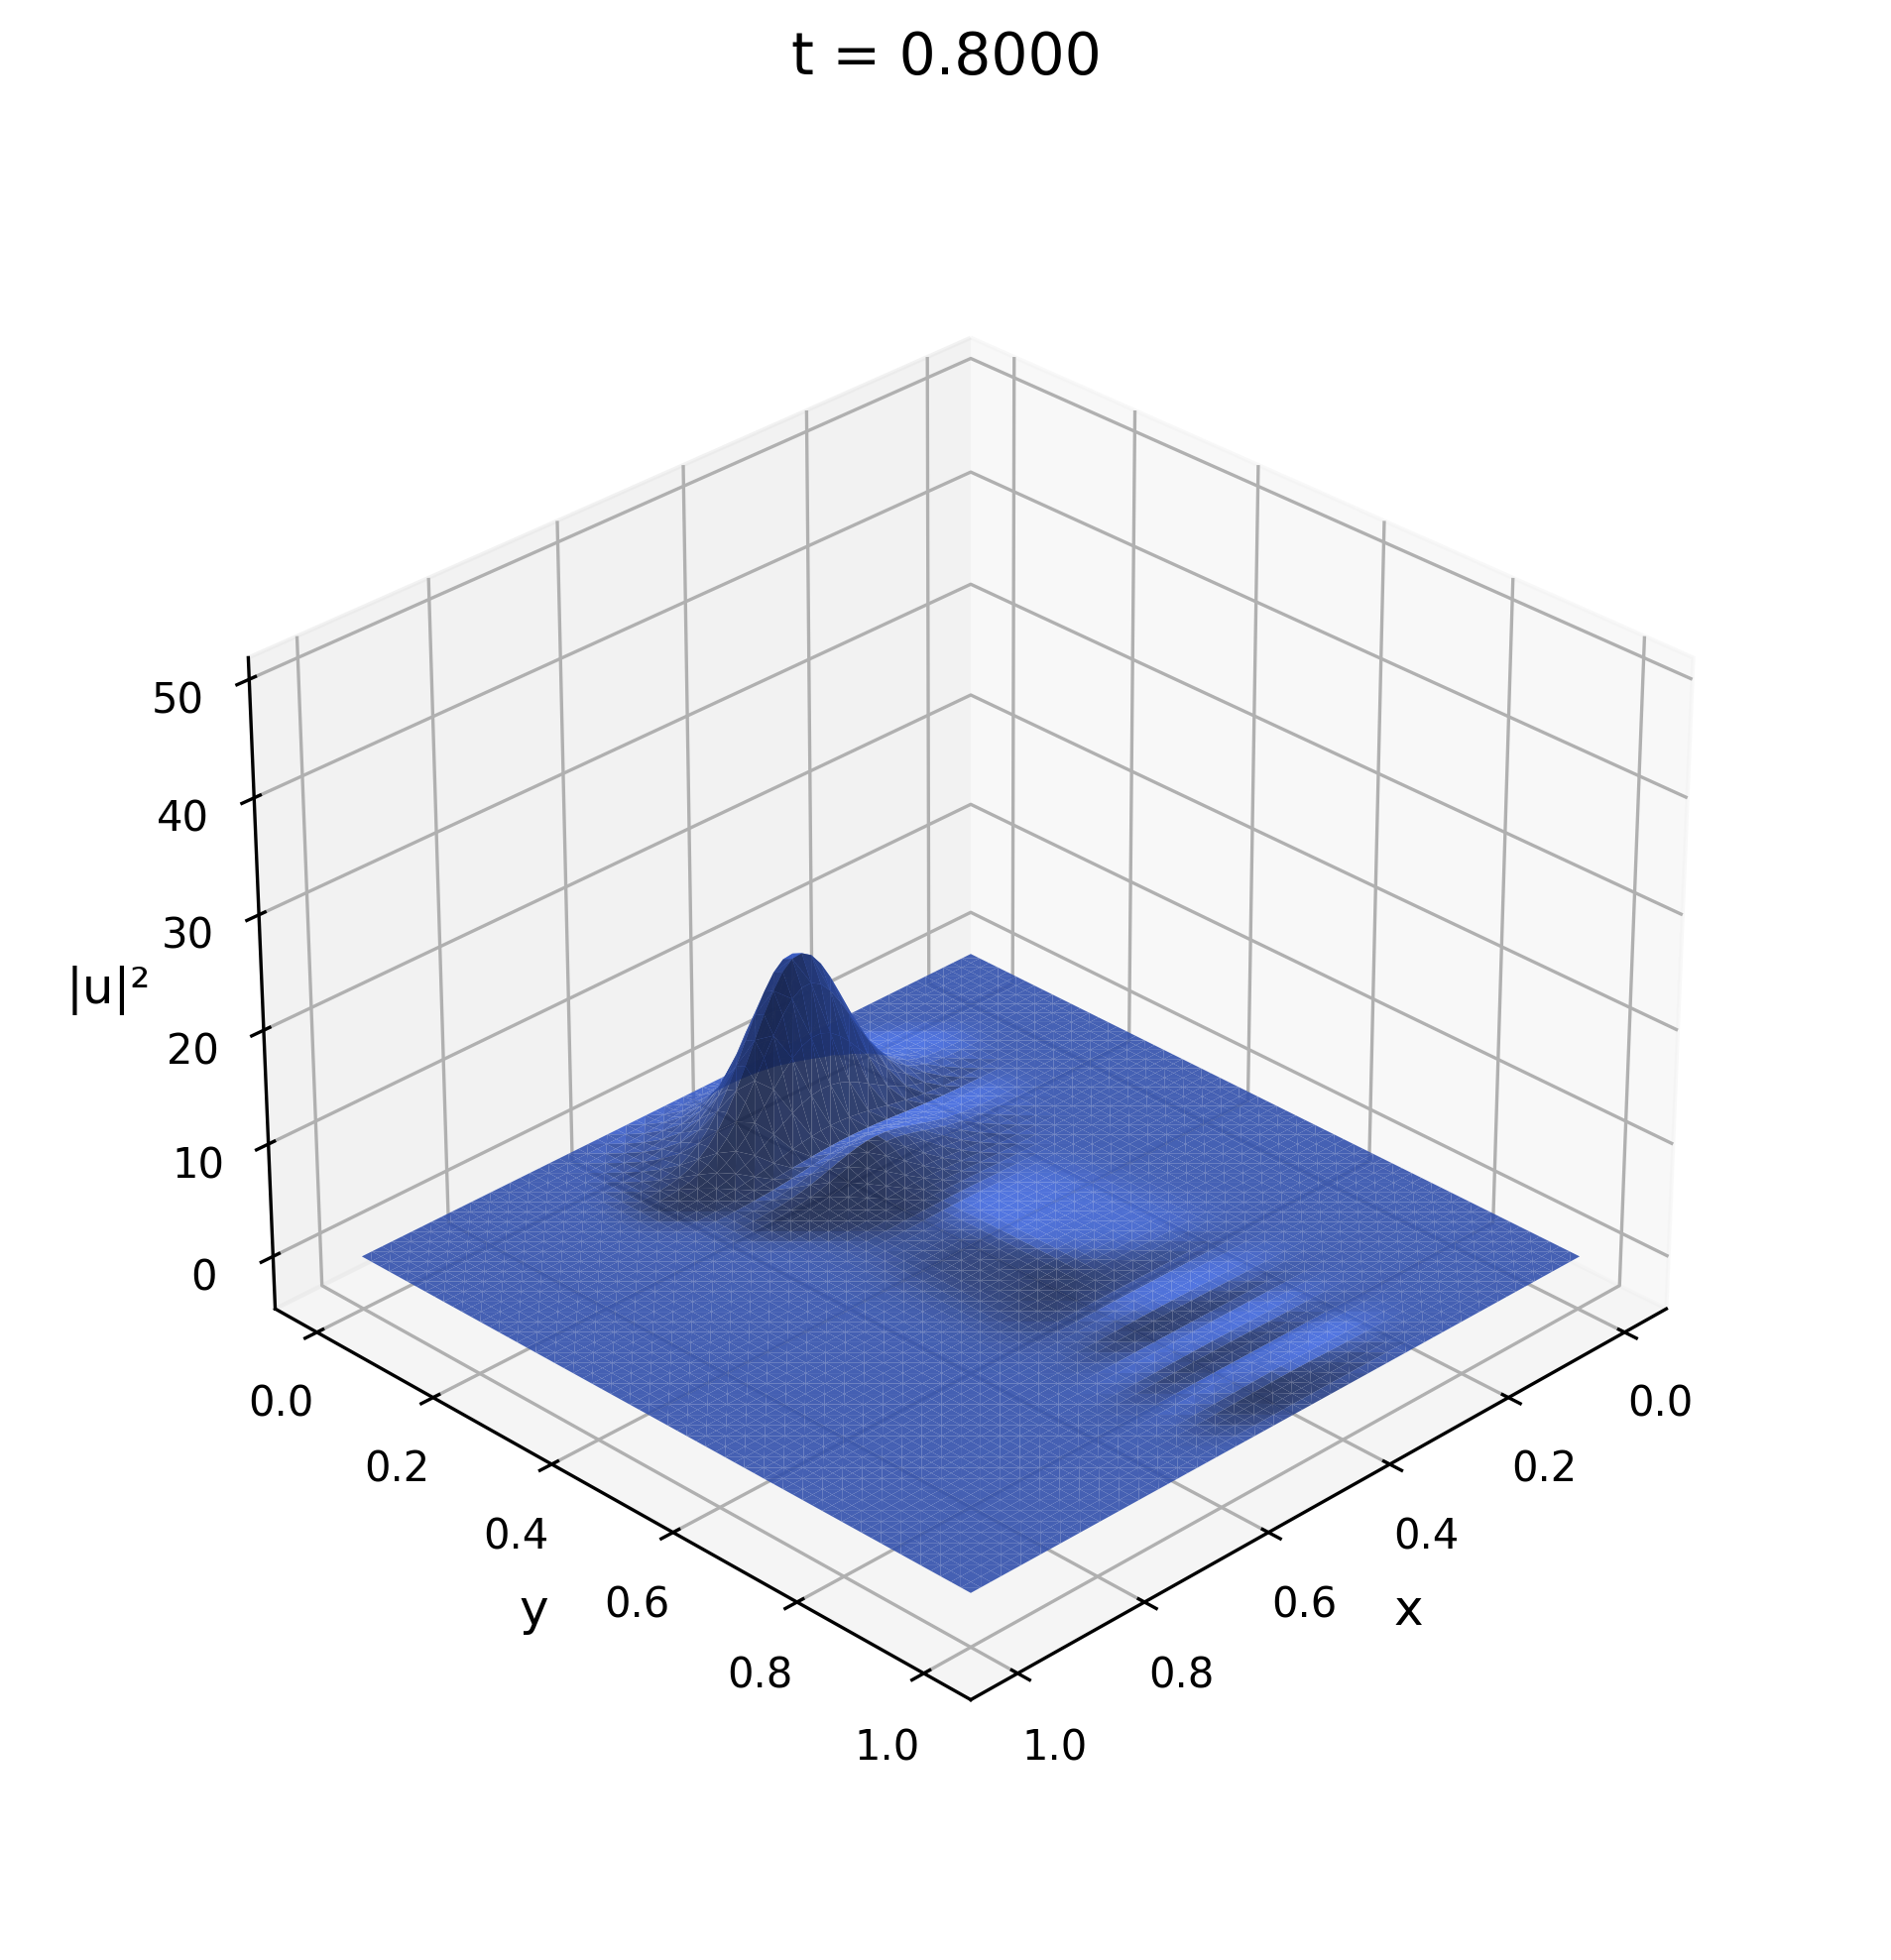
\includegraphics[width=\textwidth, trim=0cm 0cm 0cm 1cm, clip]{figures/fem_potential_frame_0080.png}
    \caption{t = 0.8}
  \end{subfigure}
  \hfill
  \begin{subfigure}[b]{0.3\textwidth}
    \centering
    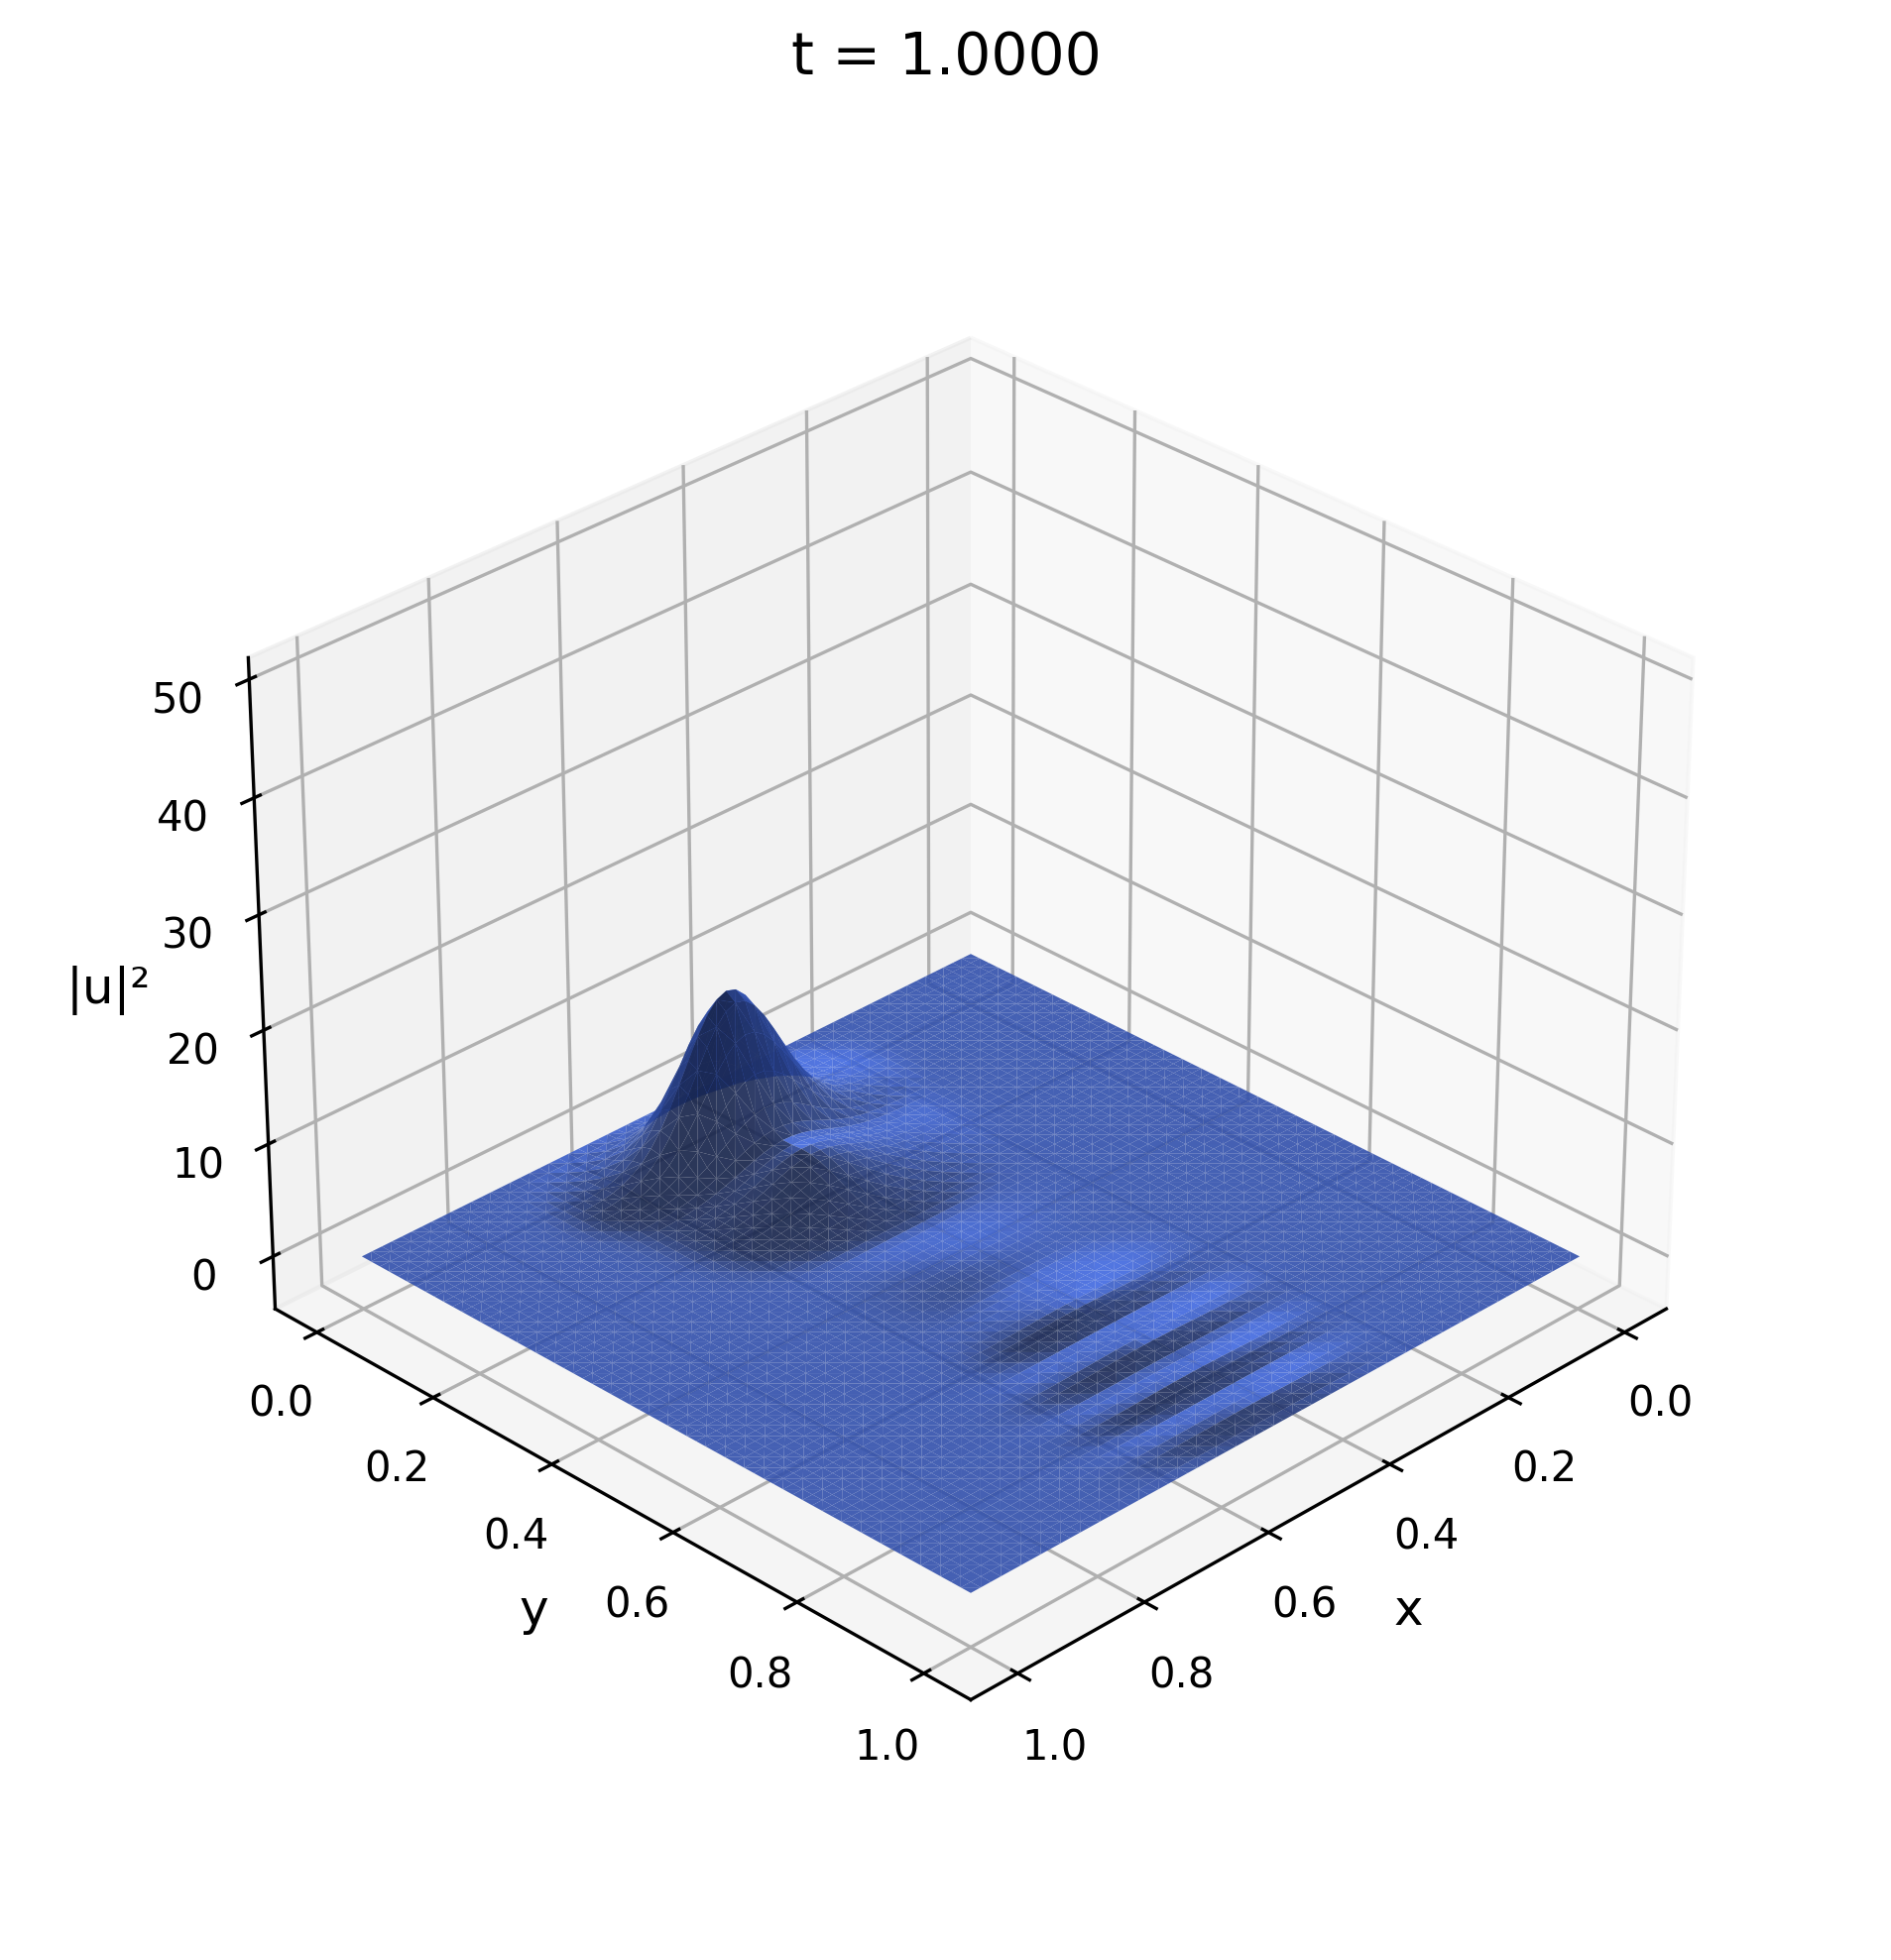
\includegraphics[width=\textwidth, trim=0cm 0cm 0cm 1cm, clip]{figures/fem_potential_frame_0100.png}
    \caption{t = 1.0}
  \end{subfigure}
  \caption{Time evolution of the solution of the Schrödinger equation with the time-dependent model potential, obtained with the FEM.}
  \label{fig:potential_evolution_fem}
\end{figure}




\section{Outlook}

We can of course only evaluate the error of FEM and PINNs for the case where we have no potential, as we know the exact solution for this case.

\subsubsection*{Spacial Error Analysis}

Here we show our numerical results for the error as a function of grid spacing with the FEM. We observe the expected convergence rate of $\mathcal{O}(h^2)$ for the FEM, except for very small grid spacings. For the PINNs, there is obviously no spacial error, as we dont use a grid.

\subsubsection*{Time Error Analysis and Energy Preservation}

Here we show that for FEMs, the error in time is of order $\mathcal{O}(\Delta t)$ for the backward Euler method and that backward Euler does not preserve the energy of the system. This could also be connected to the boundary conditions, as with the Dirichlet boundary conditions, we have implicitly also assumed von Neumann boundary conditions. Possible improvements: Crank-Nicolson method and higher order time discretization schemes, as well as using periodic boundary conditions?

For PINNs, we observe that the error in time oscilates in time, which could be due to the fact that real and imaginary parts of the solution are not learned equally well. Under ideal conditions, the error should be constant in time.

\subsubsection*{Experiments on the time-dependent Model Potential}

Here we show how the solutions of FEM and PINNs on the time-dependent model potential, for which there is no exact solution. 





\end{document}